% !TEX encoding = UTF-8 Unicode
% !TEX root = ./main.tex
% !TeX program = luatex
% !BIB TS-program = biber

% This file is MIT-Thesis.tex, a LaTeX template for formatting an MIT thesis with the mitthesis class.
%
% Version: 1.14, 2024/07/19
%
% Author: John H. Lienhard, copyright 2024. Reuse under the MIT license: https://ctan.org/license/mit 

% Documentation is here: https://ctan.org/pkg/mitthesis

%% Don't modify the \DocumentMetadata command unless you know what it does. 
%% If this command throws an "undefined" error, your latex system is out of date: try commenting this command out.
\DocumentMetadata{ 
	pdfstandard = a-2b,
	pdfversion  = 1.7,
	lang		= en-US,
%	 pdfversion  = 2.0,
%    pdfstandard = a-4,
%	 debug		= {xmp-export}, % uncomment to output a separate xmpi file showing the metadata
}

%%%%%%%%%%%%%%%%%%%%%%%%%%%%%%%%%%%%%%%

\documentclass[twoside, mydesign, fontset=heros-stix2 ,]{mitthesis} %,fontset=libertine, fontset=newtx-sans-text, fontset=heros-stix2, fontset=stix2
%
% option [twoside]		gives facing-page behavior for printing; omitting twoside will eliminate even-numbered blank pages.
% option [lineno]	 	provides line numbers, as for editing
% option [mydesign] 	loads packages for color, title and list formats, margins, or captions: edit mydesign.tex to change defaults.
% option [fontset] is a keyvalue which can be:
%					 	for pdftex or unicode engines:  defaultfonts, libertine, lucida
%					 	for pdftex only: 				fira-newtxsf, newtx, newtx-sans-text
%						for unicode engines (luatex):	heros-stix2, stix2, termes, termes-stix2
%					 	if no key value is given, fonts default to CMR (pdftex) or LMR (unicode), i.e., "the LaTeX font".
%					 	You can edit the fontset files or you can write your own, myfonts.tex, and do [fontset=myfonts].
%						If you are using multiple languages, load the babel package in your fontset file, before the fonts.

\usepackage{preamble}

\begin{document}

%%% edit the following commands to match your thesis %%%%%%%%%%

\title{Programming Methodologies and Applications on a Multipurpose Reconfigurable Photonic Integrated Platform}

% \Author{Author full name}{Author department}[Author's first PREVIOUS degree][Author's second PREVIOUS degree][...
% Note that third, fourth, fifth, and sixth arguments are optional [] and may be omitted

% note on names: most of the following names are made up; Silas Holman was a physics professor at MIT in the 19th century.

\Author{David R.
	Sánchez-Jácome}{Faculty of Telecommunications Engineering}

\Degree{Doctor of Philosophy}{Faculty of Telecommunications Engineering}
% \Author{Luisa Hernández}{Department of Research}[B.S. Mechanical Engineering, UCLA, 2018][M.S. Stellar Interiors, Vulcan Science Academy, 2020]% \Author{Thurston Howell III}{Department of Economics}[MBA, Ferengi School of Management, 2022]% Use once for each degree fulfilled by thesis% For two degrees from one department, leave the department argument blank for the second degree {}.%\Degree{Master of Science in Physics}{}%\Degree{Bachelor of Science in Mechanical Engineering}{Department of Mechanical Engineering}% If there is more than one supervisor, use the \Supervisor command for each.
\Supervisor{Daniel
	Pérez-López}{Chief Technology Officer of iPronics}
\Supervisor{José
	Capmany-Francoy}{Professor of Telecommunications Engineering}
% \Supervisor{José Capmany Francoy}{Professor of Physics, and \\ \> Professor of Something Else}
% \Supervisor{Secunda Castor}{Professor of Research}
% \Supervisor{Quintus Castor}{Professor of Log Dams}

% Professor who formally accepts theses for your department (e.g., the Graduate Officer, Professor Sméagol,...)
% If more than one department, use more than once
\Acceptor{Pascual Muñoz Muñoz}{Professor of Telecommunications Engineering}{}%{Undergraduate Officer, Department of Physics}
% \Acceptor{Tertius Castor}{Professor of Log Dams}{Graduate Officer, Department of Research}
% \Acceptor{Quarta Castor}{Professor of Lodge Building}{Graduate Officer, Department of Mechanical Engineering}
%% If you need to reduce vertical space, put the acceptor title in the second argument and leave the third blank, {}.

% Usage: \DegreeDate{Month}{year}
% Valid degree months are February, May, June, or September
\DegreeDate{July}{2025}

% Date that final thesis is submitted to department
\ThesisDate{\today}

%%%%%%  Choose whether to have a CREATIVE COMMONS License  %%%%%%%%%%%%%%%%%%%%%%%%%%%%%%%%%%%%%%
%
% If you are using a cc license, put details of your cc license here. 
% Omit this command if you are not using a cc license.
%
\CClicense{CC BY-NC-ND 4.0}{https://creativecommons.org/licenses/by-nc-nd/4.0/}
%

%%%%%%%  Solutions for overflowing titlepage  %%%%%%%%%%%%%%%%%%%%%%%%%%%%%%%%%%%%%%%%%%%%%%%%%%%

% If your title page is overflowing (from too many names, degrees, etc.):
%
% (a) you can reduce the 12pt and 18pt skips between various blocks to 6pt with this command:
%
% \Tighten
%
% (b)  you can scale down the Signature block at the bottom with this command:
%
% \SignatureBlockSize{\small}  %or this one \SignatureBlockSize{\footnotesize}
%
% (c) you can put the acceptor name and title onto two lines, rather than three like this:
%
% \Acceptor{Tertius Castor}{Professor and Graduate Officer, Department of Research}{}
%
% (d) you can change the font size of the author name[s] with
%
%	\AuthorNameSize{\normalsize}
%
% (e) and you can omit any previous degrees from the title page, instead mentioning them in the biographical sketch

% Also, if you prefer to keep the text toward the top of the page with most white space at the bottom, you
% can use this command to squash all of the vertical glue (stretchy space) with this command:
%
% \Squash 
%
% This command is useful when the text has not already reach the bottom of the page, since the glue gets squashed automatically
% when the page is too full.

%%%%%%%%%%%%%%%%%%%%%%%%%%%%%%%%%%%%%%%%%%%%%%%%%%%%%%%%%%%%%%%%%%%%%%%%%%%%%%%%%%%%%%%%%%%%%%%%%

%%% Make titlepage
\SuppressMonthError
\maketitle*

%%%%%%%%% Contents that you need to write follows! %%%%%%%%%%%%%%%%%%%%%%%%%%%%%%%%%%%%%%%%%%%%%%

% \includeonly{acknowledgments,biography,chapter1,chapter2,...,appendixa,...} 
%   for usage of includeonly, see https://latexref.xyz/_005cinclude-_0026-_005cincludeonly.html

%%% Frontmatter (write this material in the mentioned files)  %%%%%%%%%%%%%%%%%%%%%%%%%%%%%%%%%%%

% center the quote on the page
\begin{center}
	“Humans may crave absolute certainty; they may aspire to it; they may pretend, as partisans of certain religions do, to have attained it.
	But the history of science — by far the most successful claim to knowledge accessible to humans — teaches that the most we can hope for is successive improvement in our understanding, learning from our mistakes, an asymptotic approach to the Universe, but with the proviso that absolute certainty will always elude us.
	”

	\vspace{1cm}
	\textbf{— Carl Sagan}
\end{center}

\newpage{}

% Manuscript quote

% Add page with reviewers info
\textbf{Thesis Committee:}

\begin{itemize}
	\item \textbf{President:} \textit{Prof.~Pascual Muñoz Muñoz}, Faculty of Telecommunications Engineering, Universitat Politècnica de València.
	\item \textbf{Secretary:} \textit{Dr.~Angelina Totović}, Sr.~Photonics Staff Engineer, Celestial AI.
	\item \textbf{Board member:} \textit{Prof.~Mahdi Nikdast}, Faculty of Electrical and Computer Engineering, Colorado State University.
\end{itemize}

\textbf{External manuscript reviewers:}
\begin{itemize}
	\item \textbf{Reviewer 1:} \textit{Dr.~Angelina Totović}, Sr.~Photonics Staff Engineer, Celestial AI.
	\item \textbf{Reviewer 2:} \textit{Prof.~Mahdi Nikdast}, Faculty of Electrical and Computer Engineering, Colorado State University.
\end{itemize}
\newpage


% The abstract environment creates all the required headings and footers. 
% You only need to the text of the abstract in the file abstract.tex
\begin{abstract}
	% From mitthesis package
% Version: 1.01, 2023/06/19
% Documentation: https://ctan.org/pkg/mitthesis
%
% The abstract environment creates all the required headers and footnote. 
% You only need to add the text of the abstract itself.
%
% Approximately 500 words or less; try not to use formulas or special characters
% If you don't want an initial indentation, do \noindent at the start of the abstract

The field of programmable silicon photonics has garnered significant attention in recent years due to its potential to revolutionize various technological domains.
The ability to reconfigure photonic integrated circuits on demand offers unprecedented flexibility and adaptability for applications ranging from telecommunications and optical signal processing to sensing and quantum information processing.
This interest is driven by the promise of creating versatile photonic platforms that can be tailored to specific tasks through software control, much like their electronic counterparts.

This manuscript provides a comprehensive exploration of the theoretical underpinnings, the developmental journey, and the experimental validation of applications stemming from this research.
The central theme revolves around the design, implementation, and application of a multipurpose programmable photonic integrated circuit (PIC) based on a recirculating mesh architecture.
The thesis outlines the critical need for a robust technology stack, with a particular emphasis on the software infrastructure required to harness the full potential of photonic integrated circuits.
A significant portion of this work is dedicated to the in-depth documentation of various applications demonstrated on the developed photonic processor, including advancements in optical networking, tunable delay lines, optical signal processing, and topological photonics, enabled by specifically developed algorithms and high-level instructions.
Furthermore, the thesis delves into the theoretical intricacies of optical arbitrary matrix-multiply operators, proposing a novel theoretical model for Mach-Zehnder interferometers within a recirculating mesh array.
This theoretical framework is complemented by the software implementation and experimental demonstration of arbitrary parametric matrix-multiply operators on the fabricated photonic processor.
Finally, the thesis concludes by discussing the key findings, the challenges encountered and addressed, and the commercial and research prospects of the developed technology, while also outlining future directions to further the impact and accessibility of multipurpose programmable photonic platforms.
% use \input rather than \include because we're inside an environment
\end{abstract}

%% resumen.tex

% From mitthesis package
% Version: 1.02, 2024/06/19
% Documentation: https://ctan.org/pkg/mitthesis
% Author: David Sanchez-Jacome

\chapter*{Resumen}
\pdfbookmark[0]{Resumen}{resumen}

El campo de la fotónica de silicio programable ha atraído una gran atención en los últimos años debido a su potencial para revolucionar diversos dominios tecnológicos.
La capacidad de reconfigurar circuitos integrados fotónicos bajo demanda ofrece una flexibilidad y adaptabilidad sin precedentes para aplicaciones que abarcan desde las telecomunicaciones y el procesamiento de señales ópticas hasta la detección y el procesamiento de información cuántica.
Este interés se debe a la promesa de crear plataformas fotónicas versátiles que puedan adaptarse a tareas específicas mediante control por software, de forma similar a sus contrapartes electrónicas.

Este manuscrito ofrece una exploración exhaustiva de los fundamentos teóricos, el proceso de desarrollo y la validación experimental de las aplicaciones derivadas de esta investigación.
El tema central gira en torno al diseño, la implementación y la aplicación de un circuito integrado fotónico programable (PIC) multipropósito basado en una arquitectura de malla recirculante.
La tesis describe la necesidad crítica de una pila tecnológica robusta, con especial énfasis en la infraestructura de software necesaria para aprovechar al máximo el potencial de los circuitos integrados fotónicos.
Una parte importante de este trabajo se dedica a la documentación exhaustiva de diversas aplicaciones demostradas en el procesador fotónico desarrollado, incluyendo avances en redes ópticas, líneas de retardo ajustables, procesamiento de señales ópticas y fotónica topológica, gracias a algoritmos específicamente desarrollados e instrucciones de alto nivel.
Además, la tesis profundiza en las complejidades teóricas de los operadores ópticos de multiplicación matricial arbitraria, proponiendo un nuevo modelo teórico para interferómetros de Mach-Zehnder dentro de una matriz de malla recirculante.
Este marco teórico se complementa con la implementación de software y la demostración experimental de operadores de multiplicación matricial paramétricos arbitrarios en el procesador fotónico fabricado.
Finalmente, la tesis concluye analizando los hallazgos clave, los desafíos encontrados y abordados, y las perspectivas comerciales y de investigación de la tecnología desarrollada, a la vez que describe las futuras direcciones para impulsar el impacto y la accesibilidad de las plataformas fotónicas programables multipropósito.

\chapter*{Resum}
\pdfbookmark[0]{Resum}{resum}

El camp de la fotònica de silici programable ha atret una gran atenció en els darrers anys a causa del seu potencial per revolucionar diversos dominis tecnològics.
La capacitat de reconfigurar circuits integrats fotònics sota demanda ofereix una flexibilitat i adaptabilitat sense precedents per a aplicacions que abasten des de les telecomunicacions i el processament de senyals òptics fins a la detecció i processament d'informació quàntica.
Aquest interès es deu a la promesa de crear plataformes fotòniques versàtils que puguin adaptar-se a tasques específiques mitjançant control per programari, de manera similar a les contraparts electròniques.

Aquest manuscrit ofereix una exploració exhaustiva dels fonaments teòrics, el procés de desenvolupament i la validació experimental de les aplicacions derivades daquesta investigació.
El tema central gira al voltant del disseny, implementació i aplicació d'un circuit integrat fotònic programable (PIC) multipropòsit basat en una arquitectura de malla recirculant.
La tesi descriu la necessitat crítica d'una pila tecnològica robusta, amb un èmfasi especial en la infraestructura de programari necessària per aprofitar al màxim el potencial dels circuits integrats fotònics.
Una part important d'aquest treball es dedica a la documentació exhaustiva de diverses aplicacions demostrades al processador fotònic desenvolupat, incloent avenços en xarxes òptiques, línies de retard ajustables, processament de senyals òptics i fotònica topològica, gràcies a algorismes específicament desenvolupats i instruccions d'alt nivell.
A més, la tesi aprofundeix en les complexitats teòriques dels operadors òptics de multiplicació matricial arbitrària, proposant un nou model teòric per a interferòmetres de Mach-Zehnder dins una matriu de malla recirculant.
Aquest marc teòric es complementa amb la implementació de programari i la demostració experimental d'operadors de multiplicació matricial paramètrics arbitraris al processador fotònic fabricat.
Finalment, la tesi conclou analitzant les troballes clau, els desafiaments trobats i abordats, i les perspectives comercials i de recerca de la tecnologia desenvolupada, alhora que descriu les adreces futures per impulsar l'impacte i l'accessibilitat de les plataformes fotòniques programables multipropòsit.

% Resumen and resum in Spanish and Valencia

%% acknowledgments.tex

% From mitthesis package
% Version: 1.02, 2024/06/19
% Documentation: https://ctan.org/pkg/mitthesis
% Author: David Sanchez-Jacome

\chapter*{Acknowledgments}
\pdfbookmark[0]{Acknowledgments}{acknowledgments}

\section*{\textit{The path towards this PhD}}

My incursion into the field of integrated photonics started in Fall of 2015 with an Optoelectronics course at the University of Ottawa during an exchange semester while I was pursuing an Electrical Engineering degree from my alma mater, the Universidad San Francisco de Quito, in Ecuador.
Looking back in time, this PhD thesis started back then with me telling my former Ecuadorian classmates about 'using light waveguides instead of copper wires' in integrated chips.
As a consequence, I have to start thanking my mom for pushing me into applying for an exchange program abroad.
My exchange semester in Canada was generously funded by the Canadian Global affairs office's Emerging Leaders in the Americas Program (ELAP) scholarship.
Without it, the start of my research career would not have been possible as the resources at home were not enough to cover this endeavor.
My sincere gratitude to this program that helps LATAM students kickstart their careers in the North American country.
The professor teaching the Optoelectronics aforementioned course was Prof.~Ksenia Dolgaleva whom I'm profoundly grateful for not only inspiring me to delve into integrated optics but also for seeing something in me.
After the course was over, she invited me to do an undergraduate internship with her research group.
My formal research experience started at this point back in summer 2015.
Thank you very much Ksenia.

After my stay in Canada I felt that my optics and photonics background had many theoretical gaps, and thus I decided I wanted to do a master's in Photonics to address this problem.
Maybe it's because wanderlust is so pervasive these days among my generation that I leaned more towards pursuing this master's in Europe.
The quest for knowledge, language learning and adventure in the old continent seemed very appealing to the younger me.
Because of this, I express my sincere gratitude to the European Union (EU) Erasmus Mundus Joint Master's Degree (EMJMD) scholarship for funding my studies and expenses at the Europhotonics program.
From Fall 2017 to Fall 2019 this program enabled me to learn and travel in France, Germany and Italy and get acquainted with the broad spectrum of photonic applications.
From lenses to spectroscopy; from optical tweezers to camera sensors; from lithography machine to machine vision.
All these fields were placed in the horizon by this program.
I'm sincerely grateful to Professor Hughes Giovannini for his support when looking for internships.
Merci Beaucoup to Dr.~Irene Wang for hosting me in Grenoble, introducing me to the field of Optogenetics and helping me realize I had a strong inclination towards software development.
Grazie mille to Dr.~Salvatore Maresca and Professor Antonella Bogoni for the introduction to photonic FMCW radars, digital signal processing and their valuable tutoring and mentoring while in Pisa.
Dankeschön to Prof.~Carsten Rockstuhl for remotely supervising and tracking my Pisa research project when so very few professors were willing to oversee this project.
Without this small selfless action I would have not travelled to Pisa and, eventually, to Valencia.
Two years had passed and after different incursions into these photonics verticals I came to understand and accept that I'm more of an engineer than a scientist.
Thus, I settled on continuing my career in the optical systems field.

While searching for PhD positions and industry jobs I stumbled upon Prof.~José Capmany's work in 2020.
After contacting him, he told me about the new company he was co-founding with Dr.~Daniel Pérez López and Prof.~Ivana Gasulla Mestre.
I had very fond memories of my undergrad experience with electronic FPGAs so the concept of an Optical FPGA seemed really enticing to me.
It brought me back to the 2015's 'using optical waveguides instead of copper wires' idea with some added low-level fundamental logic on top of it to enable reconfiguration and multipurpose usage.
It seemed like the sweet spot for me and I immediately fell for the idea.
The deep tech start-up experience also seemed very appealing to me as I've always wanted to learn how to bring research to the market and contribute to it.
Another country, another adventure!
Muchas gracias Dani, José and Ivana for opening the iPronics doors to me.
Specifically, thanks a lot Dani for your direct supervision and mentoring.
You have not only taught me about programmable integrated photonics but also about entrepreneurship, people management and, more importantly, that all great things in life require perseverance and a lot of hard work.
Thank you, José, for always helping with the university bureaucracy and for providing the top-notch resources required to carry out our research activities.
Before coming to Valencia everyone who knew you told me you were "majo" (a good person).
They were right!
And we all unfortunately know this trait is seldom found in academia.
I guess it's all about trying to balance things in life.
Thank you, Ivana, for handling all the company and visa paperwork required for my arrival to Spain.
You were extremely helpful during the onboarding process and the first months.

\section*{\textit{The team}}

During the last 4.5 years at iPronics I have moved from chip layout design to pure software and application development with incursions to the lab when needed.
This experience couldn't have been as enjoyable as it has been without the iPronics team.
I joined the company as the third employee and now the headcount is close to 50.
Working on a small multidisciplinary team to go from scratch to first-of-its-kind product can be overwhelming sometimes (most often really fun) but never boring.
There are certainly so many fond memories of almuerzos, lunch breaks and late work sessions that will go untold.
There will always be a special place in my heart for the Software and Applications team (Alejandro, Alex, Carlos, Erica, Guillermo, Lluís, María, Paco, Thomas and Vicente) I worked side-by-side during most of this period.
Special thanks to Paco and Carlos for their, mostly successful, software development evangelization and valuable lessons about life, management and computer science.
My sincere thanks to our lab manager Ana Gutierrez for her mentoring on silicon photonics good lab practices.
Many thanks as well to Ana Gonzalez for always considering me to join her on exhibition trips and making me realize the value of networking and customer engagement.
Special thanks to Luis, Juan, María and Cristina from the PIC department for their support, advice and engaging conversations when I needed a break from the software room.

\section*{\textit{The students}}

During my PhD period I sought to develop my supervision skills, and therefore I accepted as many students and interns as I could fit in my agenda.
I'm profoundly grateful with each one of them because they allowed me to improve my training and management skills and, more importantly, for teaching me many valuable lessons that I would have taken a long time to learn myself.
In particular, thanks to the great Zhenyun Xie (Vicente) who did both his master thesis project and internship on optical computing and graph-based algorithms under my tutoring.
Thanks to Dr.~Ali Cem with whom we delved into the topic of thermal crosstalk characterization and compensation on photonic chips during his PhD stay at iPronics.
Many thanks to my first ever hires, Maria and Thomas, whom I had the privilege to train and land on the company.
Our work with Maria Rodriguez Losada made possible a Python API to implement floating parametric unitary operators on the first-generation Smartlight processor.
Together with Thomas Teferi Mulugeta I have learned enormously about Datacenter interconnects and their sensitivity to phenomena such as amplification, optical crosstalk and polarization handling.
Finally, merci to Nicolas Casteleyn whose work shed light into the challenge of polarization diversity circuits in integrated photonics for datacenter interconnects.

\section*{\textit{Family and friends}}

Family and friends have been of fundamental support during this PhD.
My mom has always been supportive and has pushed me to reach my goals even when turbulent times at home have arisen.
The second major support force throughout this period has been my girlfriend, now partner, Niko.
We ventured to Europe together pursuing our professional dreams.
During these years we have faced lockdowns, moved between flats and learned to support each other's growth while keeping things at home in check.
Muchísimas gracias mi querida Niko.
Thanks to my parents and brothers for their support during these years abroad.
They have made sure I have a warm refuge every time I go back home to reload my batteries.
Les quiero mucho!

Ever since I started hopping between countries for career or education reasons I learned the hard way that friends are the family one chooses for giving and receiving support while abroad.
Muchísimas gracias Germán, Tiz, Annabell, Mich, Lau, Juanma, Cas, Darwin and Alejo for being my Valencian family.
You'll forever have a place in my heart.
Thanks for sharing with me the experience of trying to start a new life in a new country.

\section*{\textit{The ones who sculpted this manuscript}}

The writing of this manuscript was carried out during the last 6 months.
Its structure and planning received valuable feedback from Luis Torrijos and Erica Sánchez from iPronics.
During the writing process, Germán Barriga provided great help with very skillful edits to the latex structure and figures in Inkscape.
Thomas Mulugeta was kind enough to serve as a proofreader and spotted many typos and pieces of text to be improved.
Tiziana Rubio is the artist behind the front cover who was able to turn my rough ideas into a beautiful design.
Dr.~Angelina Totovič, Prof.~Mahdi Nikdast and Dr.~Daniel Pérez López served as reviewers for this manuscript.
My sincere gratitude goes to them for taking the time to read this thesis and providing me with invaluable technical insights to significantly improve the text's quality.
% acknowledgments.tex (.tex extension is presumed by \include) 

%% biography.tex
%% This section is optional

% From mitthesis package
% Version: 1.02, 2024/06/19
% Documentation: https://ctan.org/pkg/mitthesis

\chapter*{Biographical Sketch}
\pdfbookmark[0]{Biographical Sketch}{biosketch}

David Sánchez-Jácome obtained his B.Sc.in electrical engineering in 2016 from the University San Francisco de Quito (USFQ), Ecuador.
Part of these studies were undertaken at the University of Ottawa, Canada (2015).
In 2019, he finished his master’s studies in the Europhotonics consortium, obtaining the degrees of M.Sc.
in applied physics from the University of Aix-Marseille (AMU), France, and M.
Sc.
in optics and photonics from the Karlsruhe Institute of Technology (KIT), Germany.
During the 2015-2019 period Mr.~Sánchez-Jácome has worked in different research laboratories in Canada, France, Germany and Italy.
From 2020 he has worked as a software and application lead at iPronics, where he has pursued an industrial Ph.D.
degree in collaboration with the Photonics Research Labs (PRL) of the Universitat Politècnica de València (UPV).
His current work focuses on developing advanced routines and applications for integrated software-defined photonic technologies and performing technology intelligence studies on how to bring these solutions to the market.
% biography.tex (optional, see https://libraries.mit.edu/distinctive-collections/thesis-specs/#format)

%%% Table of contents and lists of stuff (delete unused lists, i.e., if no tables or figures) %%%%%

\tableofcontents
\listoffigures
\listoftables

%%% Chapters of thesis  %%%%%%%%%%%%%%%%%%%%%%%%%%%%%%%%%%%%%%%%%%%%%%%%%%%%%%%%%%%%%%%%%%%%%%%%%%%

%% If you want to use "double spacing", you should start here...

% Author: David Sanchez-Jacome

\chapter{Introduction and objectives} \label{chap:intro}

\section{Integrated circuits} \label{sec:integrated_circuits}

Electronic integrated circuits (ICs) have revolutionized the last decades due to their ability to integrate a vast number of functionalities into a small physical space, leading to significant reductions in cost, power consumption, and increases in speed and reliability.
With the invention of the transistor this solid-state device replaced bulky and less efficient vacuum tubes, enabling miniaturization \cite{bardeen_transistor_1948}.
This in turn led to the development of the first integrated circuit \cite{kilby_invention_1976, riordan_crystal_1997}.
This innovation allowed for the fabrication of multiple interconnected electronic components on a single semiconductor substrate, paving the way for complex systems on a chip.
At the same time, continuous advancements in lithography enabled the fabrication of increasingly smaller and more densely packed transistors, as described by Moore's Law, leading to exponential growth in computing power and functionality \cite{moore_cramming_2006}.
The development of CMOS (complementary metal-oxide-semiconductor) technology offered low power consumption and high integration density, making it the dominant technology for modern ICs \cite{wanlass_low_1967}.
CMOS made possible the invention of the microprocessor \cite{noauthor_announcing_nodate}.
This milestone integrated the central processing unit (CPU) of a computer onto a single chip, enabling the personal computer revolution and the proliferation of digital technologies.
Building on the density offered by CMOS, the focus has also expanded from monolithic integration on a single chip to system-level integration through advanced packaging \cite{tummala_fundamentals_2001}.
This approach allows multiple, often specialized, integrated circuits (known as 'chiplets') to be combined into a single compact and high-performance package, pushing the boundaries of miniaturization and functionality even further \cite{naffziger_22_2020}.
These advancements have collectively driven the ubiquity of ICs across diverse fields by enabling complex information processing, communication, and control in increasingly smaller, cheaper, and more energy-efficient devices.

In parallel to the growth of electronic hardware, software has played a pivotal and increasingly significant role in the trajectory of integrated circuits from their inception to their pervasive presence in modern life.
Initially, software was crucial for the design, simulation, and testing of these nascent integrated circuits.
As IC complexity grew exponentially, sophisticated Computer-Aided Design (CAD) tools, which are fundamentally software applications, became indispensable for engineers to manage the intricate layouts and functionalities of microchips \cite{lienig_fundamentals_2021}.
Beyond the design phase, software is the very essence that provides ICs with purpose and enables their application in everyday activities.
This is possible due to layered architecture adopted for software buildup \cite{tanenbaum_structured_2013} (see Figure~\ref{fig:ch1-abstraction_layers} for an example of software layers).
At the lowest level, firmware and microcode reside directly within the IC itself, controlling the fundamental hardware operations and basic functionalities \cite{hennessy_computer_2017}.
The operating system acts as an intermediary layer, managing the IC's resources and providing a standardized platform for software applications \cite{tanenbaum_modern_2009}.
Device drivers enable the operating system to communicate with specific hardware components, translating generic commands into device-specific instructions \cite{corbet_linux_2005}.
Libraries and Application Programming Interfaces (APIs) offer collections of reusable code and standardized interaction methods, abstracting hardware complexities for application developers \cite{gamma_design_1994}.
Finally, applications are the user-facing software programs that perform specific tasks, leveraging the underlying software stack and the capabilities of the ICs to deliver their intended functionalities.

\begin{figure}
	\begin{center}
		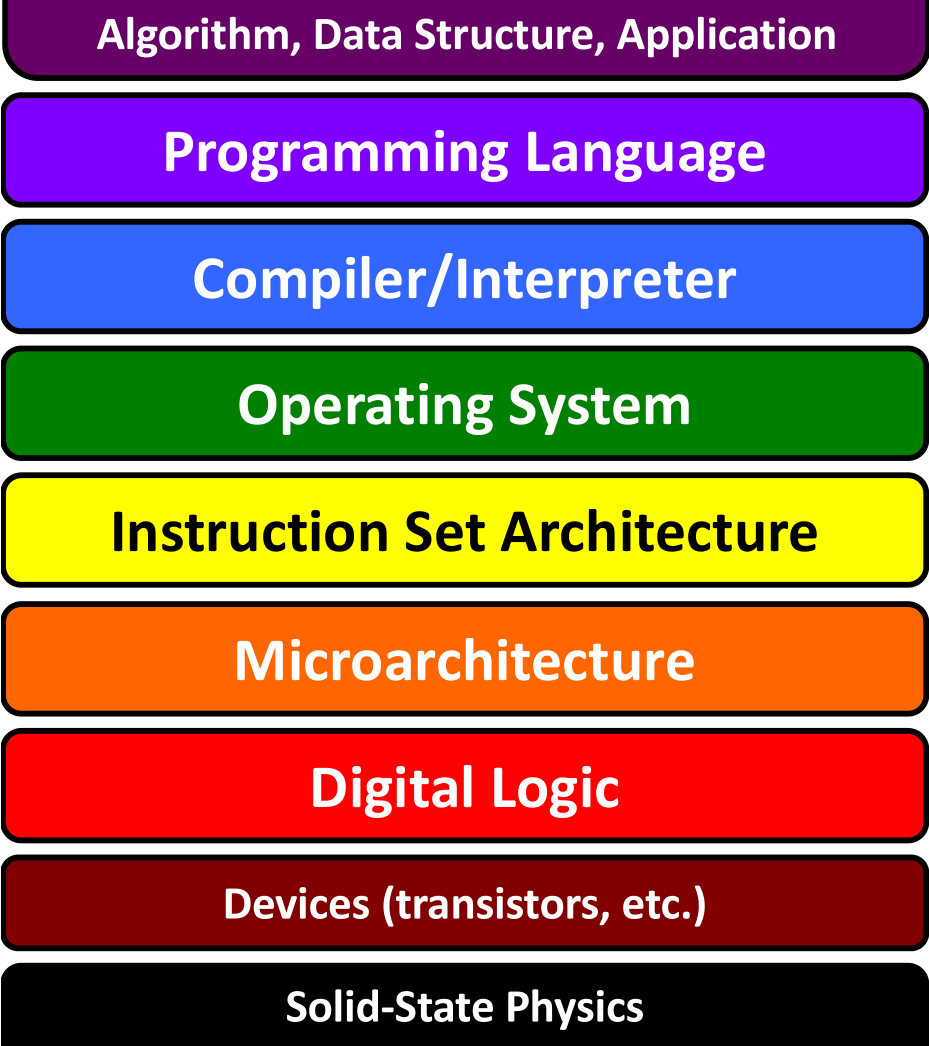
\includegraphics[width=0.35\textwidth]{figures/ch1-abstraction_layers.png}
	\end{center}
	\caption{Diagram of software abstraction layers of a typical computer system \cite{ondich_cs_2022}}\label{fig:ch1-abstraction_layers}
\end{figure}

Consequently, software stacks have democratized ICs because of their ability to translate physical semiconductor variables into human-readable instructions that can be reused and built upon.
In other words, while integrated circuits provide the physical substrate for computation and control, it is the multifaceted layers of software that orchestrate their operation, manage their resources, and ultimately translate their capabilities into the diverse array of technologies that underpin our daily lives.
The advancements in software have been unavoidably linked to the increasing power and versatility of ICs, creating a symbiotic relationship between them that continues to drive technological progress.

\section{The case for programmable integrated photonics} \label{sec:photonics_motivation}

While electronic ICs have undeniably transformed society, photonic integrated circuits (PICs) have gained significant interest and research focus due to their potential to overcome fundamental limitations of electronics and enable entirely new functionalities \cite{soref_past_2006,ye_review_2013,baets_silicon_2017}.
The motivation stems from several key factors.
Photonics inherently offers significantly higher bandwidth and lower latency for data transmission compared to electronics.
Indeed, the vast global infrastructure built upon optical fiber has demonstrated the immense capacity and efficiency of transmitting information using light.
This success naturally creates a compelling need to develop integrated photonic technologies that can efficiently interface with optical fiber and manipulate these optical signals using PICs.
As light propagates at higher speeds and with less loss in optical fibers and waveguides, PICs have become ideal for applications requiring massive data throughput, such as AI/ML data center and high-performance computing interconnects \cite{khani_sip-ml_2021,li_silicon_2015,zhou_development_2018}.
In terms of power consumption, optical communications and analog signal processing can be more energy-efficient than their electronic counterparts in certain applications, particularly over long distances (more than a few meters).
Photons do not carry an electrical charge, thus eliminating resistive losses and reducing power consumption in interconnects.
Light signals also provide immunity to electromagnetic interference (EMI) which gives photonic circuit a significant advantage in, otherwise noisy, electrical environments.
It's important to note that PICs can also be reconfigured through software just like electronic ICs, which enables them to tackle several real-life problems.
The latter fact makes them attractive for applications in microwave photonics \cite{chen_silicon_2017,marpaung_integrated_2019}, Lidar/Radar \cite{hashemi_review_2022,serafino_toward_2019}, or aerospace \cite{hsu_free-space_2022}, where signal integrity is paramount.
PICs also offer high sensitivity and precision for applications in environmental monitoring (e.g., gas and chemical sensing) \cite{chrostowski_silicon_2012}, biomedical diagnostics (e.g., lab-on-a-chip devices) \cite{fathpour_silicon_2011}, and precision metrology (e.g., optical gyroscopes) \cite{weimann_silicon_2017,khial_nanophotonic_2018}.
Likewise, reconfigurable PICs have also emerged as a promising platform for realizing complex and scalable quantum computing and communication networks \cite{harris_large-scale_2016,sibson_integrated_2017}.
All in all, similarly to electronic ICs, PICs allow for the integration of numerous optical components onto a single chip, leading to smaller, more robust, and potentially lower-cost devices.
This miniaturization facilitates the deployment of photonic technologies in a wide range of applications that demand increasingly better speed, bandwidth, power efficiency, and sensitivity specs.

% TODO: Choose if something can be added
% If we focus on data transmission, in essence, the motivation for studying and researching PICs lies in their potential to address the evolving demands for speed, bandwidth, energy efficiency, and sensitivity in information technology and beyond.
% They represent a paradigm shift that is poised to complement and, in some cases, surpass the capabilities of traditional electronics, paving the way for future technological advancements.
% One clear arena where PICs have had this success is the datacom interconnect world.
% For instance, instead of converting optical signals to electrical signals for processing and then back to optical for further transmission, PICs can perform functions like switching, routing, modulation, and detection directly in the optical domain.
% Thus avoiding energy-intensive and bandwidth-limiting optical-to-electrical-to-optical (O-E-O) conversions.
% Seamless integration with fiber optic networks is possible through PICs that can be designed to be directly compatible with optical fibers, facilitating efficient coupling and interconnection.
% This addresses bottlenecks in optical networks as the nodes and intermediate points in optical networks often rely on bulky and power-hungry discrete optical components.
% PICs offer a path towards more compact, energy-efficient, and scalable solutions for these network elements.
% Therefore, the motivation for PICs is strongly tied to the existing success of optical fiber.
% PICs represent the logical next step in leveraging the power of photonics for information handling, extending the benefits of optical communication into the integrated circuit domain and paving the way for more efficient and powerful optical networks and systems.

In a context were most of PICs are tailored for a single application, multipurpose programmable PICs based on recirculating meshes represent a significant advancement in integrated photonics.
They have garnered considerable research interest over the last decade due to their unique capabilities and potential to revolutionize various applications.
These circuits distinguish themselves through their ability to be reconfigured for diverse functionalities on a single chip, offering a level of versatility that is highly desirable in modern photonic systems \cite{bogaerts_programmable_2020,capmany_programmable_2020,perez_multipurpose_2017}.
The key distinct feature of these PICs is their architecture, which typically consists of an interconnected network of fundamental programmable elements, such as Mach-Zehnder Interferometers (MZIs) or phase shifters, arranged in a grid-like mesh.
The crucial aspect is the "recirculating" nature of these meshes, allowing light to traverse the network through a wide set of configurations.
By precisely controlling each individual element, light can be routed along various paths and cycles within the mesh to be split, combined, and phase-shifted with remarkable flexibility.
This intricate control over the optical path allows for the implementation of a wide range of linear optical transformations, which form the foundation of many photonic applications.
Furthermore, the mesh structure is scalable within the application's insertion loss budget and reticle size limits.
Therefore, increasing the number of interconnected elements allows for the creation of more complex circuits capable of tackling increasingly complex tasks.

As stated previously, for integrated solutions to become ubiquitous they must be controllable via software and PICs are not the exception.
The importance of reconfigurable multipurpose PICs largely mirrors the motivations behind reconfigurable electronic platforms like field programmable gate arrays (FPGAs) and their synergy with software control.
Reconfigurability in PICs is crucial for application testing and prototyping because it enables a single PIC to be adapted to different functionalities or changing operational requirements after fabrication.
This is particularly valuable in dynamic environments such as telecommunications networks, where traffic patterns and service demands can fluctuate.
A reconfigurable PIC can be dynamically adjusted on-the-fly to service different scenario needs.
In the case of multipurpose PICs, hardware reconfigurability significantly speeds up the prototyping and development process of new photonic systems.
Instead of designing and fabricating a new chip for each iteration or different application, researchers and engineers can program this reconfigurable PIC to test various designs and functionalities.
This reduces time-to-market and lowers development costs.
Similarly, a reconfigurable PIC can be utilized for a wider range of applications or tasks compared to a fixed-function PIC.
This leads to better resource utilization and reduces the need for multiple specialized chips, potentially lowering overall system cost and complexity.
Following the footsteps of electronic ICs, where reconfigurability enables a higher level of abstraction and control through software, comes the impending need of developing software-defined photonics.
Just as software engineers can program electronic systems without needing deep knowledge of the underlying hardware, software interfaces for reconfigurable PICs allow users to define and control complex photonic functionalities through programming interfaces.
As a consequence, the motivation behind reconfigurable PICs, under this thesis framework, is to introduce a level of flexibility and programmability into the photonic domain that mirrors the power and versatility that software brings to electronic hardware.
This allows for greater adaptability, faster innovation, and broader applicability of photonic integrated circuit technology.
In other words, if multipurpose programmable PICs are empowered with a robust and user-friendly software stack, this programmability key holds the promise to unlock a vast array of possibilities on a single photonic hardware platform.

\section{Objectives} \label{sec:objectives}

Given that reconfigurable PICs are poised to become key enablers of several technologies due to the previously stated advantages, this thesis is developed under the framework of creating a commercially available multipurpose software-defined platform with a reconfigurable PIC at its core.
The aim is to create a technology stack that resembles those in the electronics world to drive and configure a reconfigurable photonic integrated circuit in order to expose a high-level application programming interface (API) to the final users of the platform.
From bottom to top, this stack should include the photonic core, the control electronics and the software that orchestrates everything and allows to map abstract high-level functionalities to the set of physical parameters driving the PIC.
With this, we aim to demonstrate how the development of a technology stack is the key to open the door for several applications powered by a single PIC architecture.

Specifically, the global objective of this industrial PhD is to contribute in creating the technology stack needed to operate a multipurpose programmable PIC and deliver it to a final user in the form of a commercial photonic processor.
The project started with the design, tape-out and submission to manufacturing of reconfigurable PICs based on hexagonal recirculating meshes.
It continued with the creation, development, and testing of a closed-loop control system that allows the configuration of the high-density programmable PIC while the manufacturing process was carried on by the foundry.
Once the semiconductor chips and the control-loop systems arrived from fabrication, the correct functioning of each one of these individual subcomponents was tested/debugged.
Subsequently, the entire photonic processor system had to be assembled ensuring correct communication and synchronization between its composing subsystems.
With the system ready, the activities focused on the development and testing of programming strategies and algorithms that allow the optimal configuration of the newly-developed high-density photonic processor.
Precisely, this part focused on developing a software layer to configure manually and automatically circuits with different functionalities on the photonic processor.
The final steps of the thesis dealt with the experimental demonstration of several applications using the same photonic processing platform: optical interconnects, reconfigurable beamsplitters, filters, tunable continuous delay lines, optical circuit switches, topological photonic arrays and optical computing architectures, among others.
A special emphasis was put on the optical computing architectures and in-depth studies were carried out to investigate the implementation and scalability of arbitrary matrix multiply operators on the photonic processor.

% section Objective (end)

\section{Structure of the thesis} \label{sec:structure}

This thesis describes the work carried out to obtain the degree of Doctor of Philosophy (PhD) in Telecommunication Engineering under the doctorate program of the Universitàt Politècnica de València (UPV).
The research has been performed at the iPronics Programmable Photonics premises and the Photonics Research Labs (PRL) facilities at the UPV under the supervision of Dr.~Daniel Pérez-López and Prof.~Dr.~José Capmany.

The organization of this manuscript aims to provide a complete overview of the theoretical fundamentals, the development process and the experimental demonstration of application behind the research work done.
This document is subsequently structured in the following chapters:

\begin{itemize}
	\item Chapter 1: \nameref{chap:intro} provides context to the reader and goes through the motivation behind programmable integrated photonics.
	      The need for a technology stack and, particularly, software for photonic integrated circuits is outlined.
	      The main goals of this doctoral thesis and the roadmap taken during the last 4+ years are detailed.
	\item Chapter 2: \nameref{chap:fundamentals} covers the theoretical background required by the reader to understand the research developments.
	      This chapter explores the fundamentals of integrated photonics and the building blocks used to build our recirculating mesh PIC architecture.
	      This section explores in depth the technical specifications of the photonic processor platform developed under the framework of this thesis.
	      It finishes making emphasis on the software stack needed to run the system and implement the end-user applications of interest.
	\item Chapter 3: \nameref{chap:applications_using_fppgas} introduces the reader to an in-depth documentation of the applications demonstrated on the photonic processor.
	      The chapter provides a technical insight into the algorithms and high-level instructions developed during this thesis to enable different applications.
	      The applications demonstrated span over field such as optical networking, tunable delay lines, optical signal processing, topological photonics, among others.
	\item Chapter 4: \nameref{chap:universal_unitary_operators} explores the topic of optical arbitrary matrix-multiply operators in technical detail.
	      This chapter covers an extensive theoretical work carried out to make this application possible.
	      Particularly, the importance of this chapter lies on proposing a new theoretical model for MZIs within a recirculating mesh array.
	      This section finishes showing the software implementation and experimental demonstration of arbitrary parametric matrix-multiply operators on the photonic processor.
	\item Chapter 5: \nameref{chap:discussion_and_conclusions} outlines the main findings of this thesis as well as discusses the main challenges encountered and addressed during the development process.
	      Furthermore, it discusses the prospects of the photonic processor technology developed from a commercial and R\&D point of view.
	      The discussion is closed by providing a glance at the next challenges that must be solved and developments that must be done to boost the impact and democratization of multipurpose programmable photonic platforms.
\end{itemize}

At the end of the manuscript, a section is provided with a complete list of the Author’s merits and contributions to scientific journals and conferences.
% .tex extension is presumed
% Author: David Sanchez-Jacome

\chapter{Fundamentals of Programmable Integrated Photonics} \label{chap:fundamentals}

The evolution of integrated photonics has led to the development of programmable photonic circuits, enabling flexible and reconfigurable optical signal processing.
Unlike fixed-function photonic circuits, programmable architectures provide the ability to dynamically adapt their functionality.
This chapter explores the fundamental components that form the foundation of programmable integrated photonics.
We begin by examining the building blocks of these circuits, including optical waveguides, phase shifters, and couplers, which serve as the core elements for light manipulation.
Next, we delve into recirculating photonic meshes, the scalable architectures that enable complex optical transformations through interconnected tunable elements.
Following this, we introduce iPronics first-generation Smartlight solution, a leading implementation of general-purpose programmable photonics, demonstrating the transition from academic research to real-world applications.
Finally, we discuss the software stack that enables seamless control of these photonic processors, bridging the gap between hardware and high-level applications.

\section{Building blocks} \label{sec:building_blocks} % (fold)
\subsection{Optical waveguides} \label{sub:optical_wg} % (fold)

\begin{figure}[h]
	\begin{center}
		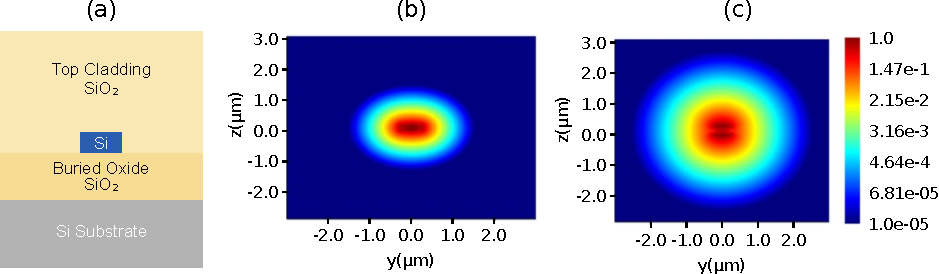
\includegraphics{figures/ch2-wg.pdf}
	\end{center}
	\caption{Optical strip waveguide. (a) Material cross-section showing the high-index \ce{Si} core surrounded by the \ce{SiO2} cladding. (b) and (c) show the first TE and TM propagation mode's field
		intensity, respectively.}\label{fig:ch2-wg}
\end{figure}

Integrated optical waveguides are the foundational components of photonic integrated circuits (PICs), enabling the propagation of optical signals within a confined medium.
Structurally, waveguides function as optical counterparts to electrical transmission lines, utilizing total internal reflection (TIR) to guide light through a high-refractive-index core surrounded by a lower-refractive-index cladding.
The most prevalent waveguide configurations include strip waveguides, which are fully etched channels embedded in a planar substrate, and rib waveguides, which feature a partially etched ridge atop a lower-index slab, providing enhanced modal confinement and reduced propagation losses.
These structures can be fabricated from a variety of materials, including silicon \cite{siew_review_2021}, silicon nitride \cite{xiang_silicon_2022}, indium phosphide \cite{smit_past_2019} and lithium niobate \cite{boes_lithium_2023}, each offering distinct advantages in terms of propagation loss, nonlinearity, and compatibility with complementary metal-oxide-semiconductor (CMOS) processes.
One of the main key issues addressed by fabrication foundries is insertion losses (IL) of the waveguides.
The minimization of this parameter from a couple of \(dB/cm\) to \(dB/m\) is crucial in enabling large-scale photonic integration.
This, in turn, will make possible the that integrated applications can compete directly with existing free-space solutions.

Integrated waveguides serve a critical role in modern photonic systems, facilitating functionalities such as optical signal routing, modulation, switching, and multiplexing.
Through different design geometries they can take the form of devices like Mach-Zehnder interferometers (MZIs), micro ring resonators (MRRs), delay lines (DLs), among many others.
Figure~\ref{fig:ch2-wg} depicts the cross-section of an optical waveguide used in the first-generation Smartlight platform (a).
This waveguide has a width of 0.5~um and a height of 0.22~um and a typical loss of 2.5~\(dB/cm\) in the C-band \cite{perez-lopez_general-purpose_2024}.
Next to it in (b) and (c) we observe the simulated field distribution for the first TE and TM modes respectively.
For further theory related to light confinement in semiconductor waveguides refer to \cite{chrostowski_silicon_2015,saleh_guided-wave_1991}.
% subsection Optical waveguides (end)

\subsection{Splitters}\label{sub:splitters} % (fold)

\begin{figure}[h]
	\begin{center}
		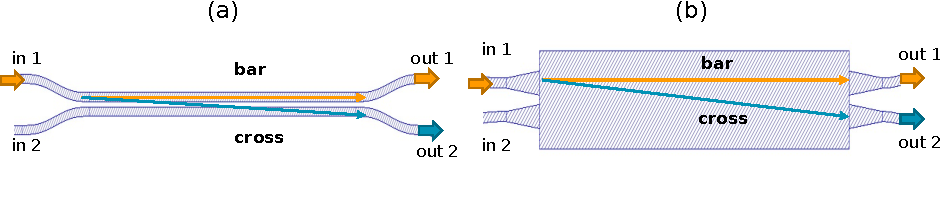
\includegraphics{figures/ch2-splitters.pdf}
	\end{center}
	\caption{Schematic representation of a directional coupler (DC) (a) and a multimode interferometer (MMI) (b) used to split optical signals.}\label{fig:ch2-splitters}
\end{figure}

Optical splitters are passive photonic devices that divide or combine optical signals in integrated photonic circuits.
They are fundamental building block to perform to efficient and low-loss signal distribution and routing.
In integrated photonics, two of the most commonly used optical splitters are Directional Couplers (DCs) and Multimode Interferometers (MMIs).

Directional Couplers (DCs) are passive components that use evanescent coupling between two adjacent waveguides to perform the splitting operation.
When these two optical waveguides are placed close together (typically a few hundred nm) their evanescent fields overlap, allowing light to tunnel from one waveguide to the other.
This phenomenon, known as evanescent coupling, is the fundamental mechanism behind directional couplers \cite{tormen_wavelength-flattened_2005,chen_broadband_2017,chen_low-loss_2016}.
Because of this, DCs are highly dependent on wavelength, waveguide separation, and coupling length.
Similarly, the dependence on very small waveguide gaps makes them sensitive to small variations in waveguide fabrication.
In terms of footprint, they are typically longer than MMIs as they are restricted by the coupling length.
One advantage over MMIs is that they can be tuned dynamically via phase shifters to control its output phase and amplitude response \cite{perez-lopez_integrated_2019}.
DCs usually yield lower insertion loss (\(IL = [0.1, 0.5]\) dB) but are susceptible to coupling imbalances due to fabrication tolerances \cite{darmawan_rigorous_2005}.

A Multimode Interferometer (MMI) is a passive photonic device used for splitting, combining, and routing optical signals in integrated photonic circuits.
It operates based on self-imaging in multimode waveguides, where an input optical field forms multiple replicas at specific distances inside the waveguide due to interference between supported modes.
When light enters the multimode waveguide, it excites multiple propagation modes.
These modes interfere constructively and destructively at different points, forming periodic self-images.
Depending on the length and width of the MMI, different power-splitting ratios can be achieved \cite{soldano_optical_1995,sheng_compact_2012}.
Mathematically, the self-imaging effect in an MMI is determined by its length \( L \) and effective refractive index \( n_{\text{eff}} \), which define the position of constructive interference patterns.
These components can perform a large variety of splitting ratios (1×2, 1×N, N×M configurations) to distribute signals efficiently \cite{hosseini_1_2011}.
Unlike directional couplers, MMIs are less sensitive to fabrication variations, ensuring high yield and reliability in large-scale photonic chips.
If designed correctly these components can also occupy a small footprint which favors large-scale integration \cite{kim_experimental_2022}.
Even though MMIs introduce higher insertion losses than directional couplers (\(IL = [0.2, 0.8]\) dB), their high yield and fabrication tolerance makes them a very attractive solution for large integrated distribution circuits \cite{darmawan_rigorous_2005}.
Because of these reasons MMIs are widely used as power splitters, combiners, and switches in PICs \cite{song_low-loss_2022}.

Figure~\ref{fig:ch2-splitters} shows the schematics of both a DC (a) and an MMI (b) from one of the several chips fabricated by iPronics in the time frame of this thesis.
These components have been optimized to achieve as low-loss and small footprint as possible to favor high-density integration in our chips.
The splitter chosen for our main designs is the MMI as it provides the low-loss, fabrication tolerance and broadband specs required by the applications that will be presented in Chapter~\ref{chap:applications_using_fppgas}.

Several MMI/DC designs are simulated, sent for tape-out and characterized in our lab facilities before they are included as part of our final chips.
Typically, once the best components have been filtered out during the simulation stage, they are included in test dies that are fabbed in multiproject wafer (MPW) runs.
Once the chips, reach our facilities they are characterized in terms of insertion losses, crosstalk and reflection in order to select the best candidates that will be included in our main mesh circuits.

% subsection Splitters (end)

\subsection{Phase shifters}\label{sub:phase_shifters} % (fold)

\begin{figure}[h]
	\begin{center}
		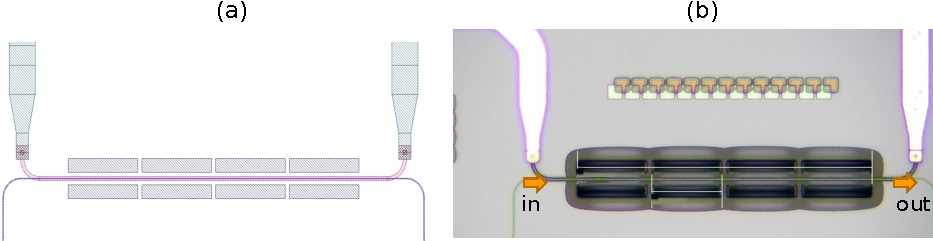
\includegraphics{figures/ch2-phase_shifter.pdf}
	\end{center}
	\caption{(a) Schematic representation and (b) microscope picture of a thermo-optic phase shifter fabricated to provide reconfigurability to the underlying PIC structure.}\label{fig:ch2-phase_shifter}
\end{figure}

A phase shifter is a key component in programmable integrated photonics.
It's responsible for modulating the phase of an optical signal as it propagates through a waveguide.
By controlling the phase of light, phase shifters enable essential functions such as beam steering, optical interference control, and signal processing in photonic circuits.
A phase shifter modifies the optical path length of a waveguide by altering its refractive index or physical length.
The phase of a light wave traveling through a waveguide is defined by:

\begin{equation}
	\phi = \frac{2\pi n_{eff}
		L}{\lambda} \label{eq:ch1-phase_shift} \end{equation}

where \( n_{eff} \) is the effective refractive index, \( L \) is the waveguide length, and \( \lambda \) is the optical wavelength in vacuum.
Changing either \( n \) or \( L \) causes a shift in the optical phase \cite{chrostowski_silicon_2015}.

There are different types of phase shifters in photonic integrated circuits:

\begin{itemize}
	\item Thermo-Optic Phase Shifters (TOPS): Based on heating a waveguide to change its refractive index.
	      They are comparably slow (µs response time), but low power and widely used in silicon photonics.
	      Commonly found in Mach-Zehnder interferometers (MZIs) and programmable photonic meshes \cite{jacques_optimization_2019, liu_thermo-optic_2022}.
	\item Electro-optic Phase Shifters: Make use of an electric field to change the refractive index through the Pockels effect.
	      Found in materials like lithium niobate (\ce{LiNbO3}) or III-V semiconductors.
	      They are much faster (ps–ns range) than thermo-optic phase shifters, making them ideal for high-speed modulators \cite{maldonado_electro-optic_1995,yoshioka_cmos-compatible_2024}.
	\item Carrier Injection/Depletion Phase Shifters: Based on using free carrier-flow (electrons/holes) to modify the refractive index.
	      Implemented in silicon photonics via PN-junctions or MOS capacitors.
	      Faster than thermo-optic phase shifters (ns range) but more lossy \cite{gabriel_performance_2020,kruckel_towards_2021}.
	\item MEMs-Based Phase Shifters: Use micro-electromechanical actuators to change the waveguide position or structure.
	      Extremely low power consumption but require high voltages and their process nodes have lower maturity/reliability.
	      Useful in tunable optical circuits and programmable photonic chips \cite{errando-herranz_mems_2020,quack_integrated_2023}.
\end{itemize}

Phase shifters are essential for dynamically controlling light in reconfigurable photonic circuits.
In the last decade they have enabled the demonstration of large array reconfigurable PICs.
These applications span the fields of optical switching for datacenter networking, beam steering phased array antennas, quantum photonics and photonic neural networks.

Figure~\ref{fig:ch2-phase_shifter} shows the schematic (a) and microscope photography (b) of a thermo-optic phase shifter deployed in the framework of this thesis.
The actuators use under-etch technology to provide thermal isolation to mitigate thermal crosstalk and provide higher rise time.
As observed in the figure, trenches have been placed next to the high resistance heating material to create air isolation around it and the underlying waveguide.
To better understand thermal crosstalk and how this design mitigates it refer to Section~\ref{sec:thermal_crosstalk}.

% subsection Phase shifters (end)
\subsection{The Mach-Zehnder interferometer}\label{sub:the_mach-zehnder-interferometer} % (fold)

\begin{figure}[h]
	\begin{center}
		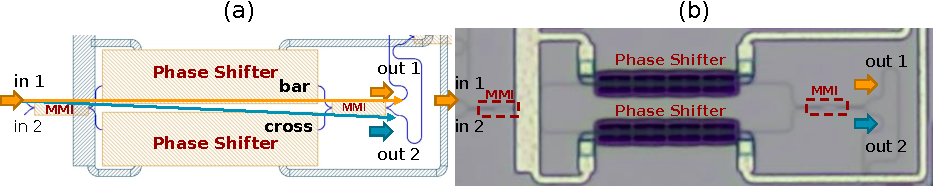
\includegraphics{figures/ch2-mzi.pdf}
	\end{center}
	\caption{Schematic representation (a) and microscope photography (b) of the fabricated MZIs.
		The chosen design uses MMIs are optical splitters and two underetched phase shifter to provide accurate control of phase and amplitude at the interferometer's output.
	}\label{fig:ch2-mzi}
\end{figure}

A Mach-Zehnder interferometer (MZI) is an optical device that splits and recombines light waves to create interference patterns.
The MZI operates by splitting an input light wave into two paths, modulating them separately, and then recombining them to analyze interference effects.
This allows precise monitoring of phase, amplitude, and wavelength of light \cite{mach_ueber_1892,zehnder_neuer_1891}.
Because of this, it is widely used in optical communication, sensing, metrology, and programmable photonics.

In free-space optics, a traditional Mach-Zehnder Interferometer consists of two beam splitters and two mirrors that create two distinct optical paths.
A coherent light source enters the first beam splitter, which divides the light into two separate beams traveling along different arms of the interferometer.
Each beam travels through its own optical path, which can include phase modulators, delay elements, or medium variations that affect the phase difference between them.
The two beams meet at a second beam splitter, where they interfere constructively or destructively depending on their phase difference.
The resulting interference pattern is measured at the output ports, providing information about path differences, refractive index changes, or external modulations \cite{saleh_wave_1991}.
Free-space MZIs are widely used in interferometric sensing, optical coherence tomography (OCT), and precision metrology, where detecting small phase shifts is critical \cite{hariharan_interferometry_2005,fujimoto_optical_2003}.

In integrated photonics, the free-space optics components (beam splitters, mirrors, and modulators) are replaced by on-chip waveguides and phase shifters.
Instead of bulk beam splitters, MMIs or DCs divide the light into two waveguide arms.
The waveguides include thermo-optic, electro-optic, or carrier-injection phase shifters, allowing dynamic phase control.
After phase modulation in the arms, the light recombines at a second waveguide splitter, producing an interference pattern that can be either detected electronically or used for further optical processing.
The advantage of integrated MZIs is that they enable high-density integration for large-scale photonic circuits, allowing for real-time reconfiguration and high-speed processing in applications like optical switching, modulators, LiDAR, quantum photonics and photonic neural networks \cite{capmany_programmable_2020}.
The concept of programmable integrated photonics (PIP) is driven by this motivation to integrate high MZI counts, and other tunable elements, to favor the development of novel photonic solutions.

Figure~\ref{fig:ch2-mzi} depicts the schematic (a) and a microscope photography (b) of one of the MZIs in the first-generation Smartlight processor.
Notice that it's composed by two MMIs (input/output) and two thermo-optic phase shifters (one per arm).
The circuit is balanced as both arms have the same length.
The two actuators allow control over the phase and amplitude response of the circuit.
From now on in this document we will refer to this type of MZI, a balanced dual-driven one, as a \textbf{programmable unit cell (PUC)} to emphasize its role as the basic reconfigurable building block for this thesis.
The transfer matrix representing a PUC for a fixed state of polarization and lossless propagation is given by Equation~\eqref{eq:ch2-puc}

\begin{equation}
	\label{eq:ch2-puc}
	\begin{aligned}
		T_{PUC} & =
		\begin{bmatrix} \sqrt{\rho} & j\sqrt{1-\rho} \\ j\sqrt{1-\rho} & \sqrt{\rho} \end{bmatrix}
		\cdot
		\begin{bmatrix} e^{j\phi_{up}} & 0 \\ 0 & \phi_{lo} \end{bmatrix}
		\cdot
		\begin{bmatrix} \sqrt{\rho} & j\sqrt{1-\rho} \\ j\sqrt{1-\rho} & \sqrt{\rho} \end{bmatrix} \\
		        & =
		je^{j\Delta}
		\begin{bmatrix}
			sin(\theta) & cos(\theta)  \\
			cos(\theta) & -sin(\theta)
		\end{bmatrix}.
	\end{aligned}
\end{equation}
where \(\phi_{up},\) and \(\phi_{lo}\) correspond to the upper and lower driving phases.
$\Delta = (\phi_{up} + \phi_{lo})/2$ is what we will refer from on as the \textbf{cross-phase}, and it's a measure of the common phase at the PUC's outputs.
$\theta = (\phi_{up} - \phi_{lo})/2$ is related to the \textbf{coupling factor \(k\)} through the \(k = cos(\theta)\) relationship.
The coupling factor is a critical metric because it defines the amplitude response of the PUC at each output.
\(\rho\) is the MMI's power splitting ratio and is considered to be 0.5 for an ideal 3-dB coupler \cite{shokraneh_theoretical_2020}.
The experimental measurement of the PUC's transfer matrix will be covered in detail later in this chapter alongside Figure~\ref{fig:ch2-sw-calib}.

\subsection{Integrated photonic resonant devices}\label{sub:integrated_photonic_resonant_devices} % (fold)
\begin{figure}
	\begin{center}
		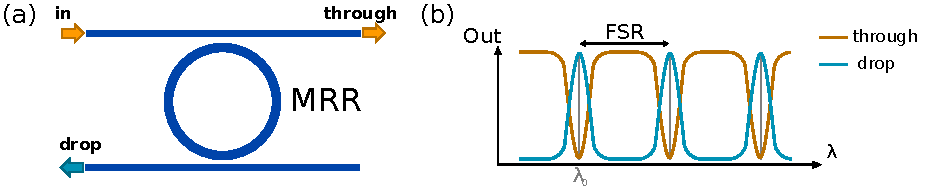
\includegraphics{figures/ch2-ring.pdf}
	\end{center}
	\caption{Basic configuration (a) of a MRR in PIC circuits.(b) Shows the optical response on the through and drop ports}\label{fig:ch2-ring}
\end{figure}

Resonant devices are key components in PICs and are designed to selectively interact with light at specific wavelengths through the principle of resonance.
They achieve this by trapping and intensifying light within an optical cavity at particular resonant wavelengths.
They are characterized by their resonant wavelength, Free Spectral Range (FSR), and Quality Factor (Q-factor).
A high Q-factor signifies a sharp, narrow resonance and excellent energy storage, crucial for applications demanding high spectral selectivity or sensitivity \cite{bogaerts_silicon_2012}.

Microring resonators (MRRs) are the most common resonant structure in silicon photonics PICs.
An MRR is essentially a waveguide formed into a closed loop, where light couples in from an adjacent "bus" waveguide via evanescent waves.
Resonance occurs when the optical path length around the ring is an integer multiple of the ring's resonant wavelength, leading to constructive interference.
When light is "on-resonance," it efficiently couples into the ring, building up intensity and appearing at a "drop" port (in an add-drop configuration) or causing a dip in the "through" port (in an all-pass configuration).
Light that's "off-resonance" passes through with minimal interaction \cite{chao_polymer_2006}.

MRRs offer several advantages: they are compact, allowing for high integration density, and can achieve very high Q-factors, leading to precise spectral filtering.
They are also highly versatile, functioning as filters, modulators, switches, and sensors.
Their resonant wavelength can be tuned using various effects, such as thermo-optic or electro-optic changes \cite{bawankar_microring_2021}.
However, MRRs do come with challenges \cite{little_toward_2000}.
Their performance is highly sensitive to fabrication variations, meaning tiny manufacturing imperfections can significantly alter their resonant properties.
They are also susceptible to temperature fluctuations due to the thermo-optic effect, often requiring active thermal stabilization.
Overcoming these challenges is a major focus in current PIC research and development.

% subsection Integrated photonic resonant devices (end)
% subsection The Mach-Zehnder interferometer (end)
\section{Recirculating Meshes}\label{sec:recirculating_meshes} % (fold)

\begin{figure}[h]
	\begin{center}
		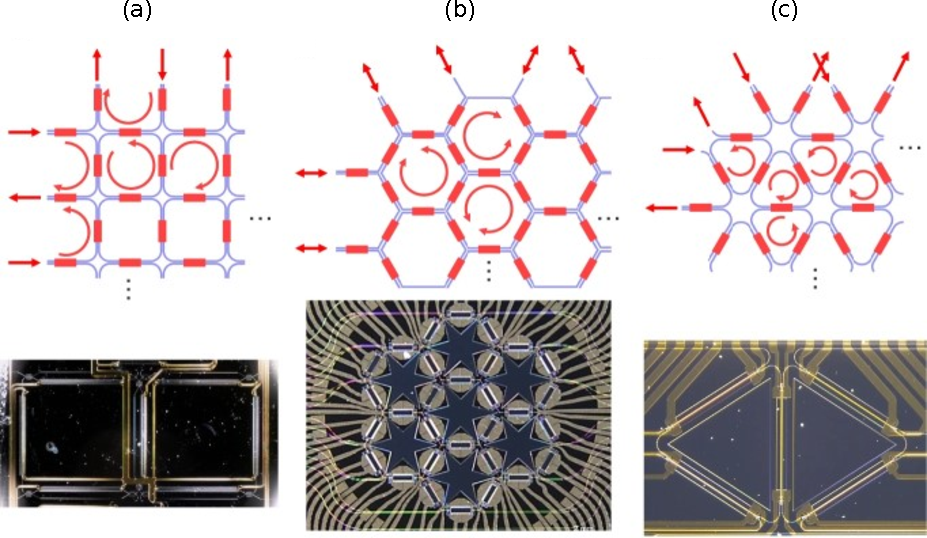
\includegraphics{figures/ch2-recirculating.pdf}
	\end{center}
	\caption{Schematic representation (top) and microscope photography (bottom) of square, hexagonal and triangular based recirculating meshes.
		Photographs reproduced from \cite{zhuang_programmable_2015}, OSA Publishing (a), \cite{perez_multipurpose_2017}, Springer Nature (b) and \cite{perez-lopez_integrated_2019}, OSA Publishing (c).
		Schematics reproduced from \cite{bogaerts_programmable_2020}, Springer Nature.
	}\label{fig:ch2-recirculating}
\end{figure}

Recirculating meshes consist of an array of PUCs coupled together using optical waveguides to create a regular a two-dimensional (2D) grid of loops.
These photonic circuit architectures incorporate feedback loops to enable complex optical transfer functions.
Unlike feedforward meshes, which rely solely on cascading interferometers, recirculating meshes introduce multi-path interference and resonant effects, providing additional functionality in filtering, delay engineering, and signal processing.
A key advantage of recirculating meshes is their ability to implement higher-order spectral filtering, making them useful in applications requiring precise wavelength selection as shown in Section~\ref{sec:filters}.
Additionally, they allow for programmable dispersion and optical delay, enabling advanced signal-processing functionalities such as optical buffering and equalization (refer to Sec~\ref{sec:reconfigurable_delay_lines}).
Their compact nature also offers benefits in circuit integration, as they provide complex operations without requiring long cascades of optical elements.
These meshes can also be programmed as forward-only arrays (although using more PUCs) as will be discussed in detail in Chapter~\ref{chap:universal_unitary_operators}.

Figure~\ref{fig:ch2-recirculating} showcases different recirculating photonic mesh architectures used in programmable photonic circuits.
It consists of square \cite{zhuang_programmable_2015}, hexagonal \cite{perez_multipurpose_2017} and triangular \cite{perez-lopez_integrated_2019} architectures (a, b, and c, respectively).
The top row presents schematic representations of the photonic meshes, where red elements correspond to PUCs, and blue lines represent optical waveguides.
The arrows illustrate the input and output ports, as well as the propagation directions of light within the structures.
The bottom row contains microscope images of the corresponding fabricated photonic chips.
When comparing these topologies \cite{perez_reconfigurable_2016-1,capmany_programmable_2020} against each other using metrics such as PUCs per area, reconfigurability, and filter periodicity (among others), the hexagonal mesh comes on top, especially because all ports can function as inputs/outputs (I/O) \cite{bogaerts_programmable_2020}.

Due to the integration complexity, these architectures introduce significant control and stability challenges.
The presence of feedback loops demands precise pre-characterization or optimization methods to prevent unwanted resonances or instability \cite{perez-lopez_multipurpose_2020,perez-lopez_programmable_2020}.
Moreover, optical losses accumulate with each round trip inside the loop, which can degrade overall performance.
In silicon photonics, where propagation losses are non-negligible, this poses a major design constraint.

Despite these challenges, recirculating meshes have found applications in programmable optical filters, optical delay lines, and reconfigurable photonic processors.
Their ability to manipulate optical signals dynamically makes them particularly valuable in telecommunications, signal processing, and even quantum photonics.
Chapter~\ref{chap:applications_using_fppgas} covers in detail the advanced programming strategies required to implement and experimentally validate several applications in the hexagonal mesh developed by iPronics for its first-generation Smartlight platform.

\section{Smartlight: The Field Programmable Photonic Gate Array}\label{sec:smartlight_fppga}

\begin{figure}[h]
	\begin{center}
		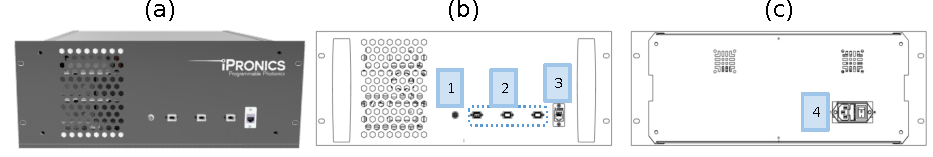
\includegraphics{figures/ch2-smartlight.pdf}
	\end{center}
	\caption{Photography of a first-generation Smartlight processor (a) and schematics of its front (b) and back panels (c).
		External interfaces are numbered: (1) Laser output, (2) Optical ports (3 MTP/MPO connectors, 72 optical ports), (3) Ethernet communication port, (4) Power supply input.
	}\label{fig:ch2-smartlight}
\end{figure}

The general-purpose photonic processor presented in this work aggregates, for the first time, the complex full-stack necessary to operate a programmable photonic device: the optical layer, the control layer, and the software layer.
The processor has been named, and will be referred hereafter, as the iPronics Smartlight Processor.
The first-generation Smartlight is contained in a 4U rack box with two front handles as shown in Figure~\ref{fig:ch2-smartlight}(a).
Fig.~\ref{fig:ch2-smartlight} (b) depicts the front panel which contains, from left to right, a ventilation hexagonal grid, a laser optical output through an FC/APC optical connector (1), three MTP optical connectors with 24 channels each (2), and a Cat-6 Ethernet female connector (3), which is physically connected to the control unit of the iPronics Smartlight processor.
The back panel, shown in Fig.~\ref{fig:ch2-smartlight}(c) contains the main power socket IEC C14 (4) located on the right side, together with an ON-OFF switch.
Also, in the upper part there are two ventilation grills holding two air fans in the inside.

\subsection{General specifications}\label{sub:general_specifications} % (fold)

The general specifications of the first-generation Smartlight system are presented in Table~\ref{tab:ch2-gen-specs} where most of the externals provisions are detailed.
Notably, the units come equipped with an internal tunable laser source to enable standalone operation without any third-party equipment.
The system consumes less than 20 W and has been designed and engineered to work in the C-band for telecom applications.

% \begin{noindent}
\begin{table}[h!]
  \small
	\centering
	\begin{tabular}{|m{4cm}|m{1.0cm}|m{1.0cm}|m{1.0cm}|m{1.5cm}|m{5.5cm}|}
		\hline
		\multirow{2}{*}{\textbf{Specification}} & \multicolumn{3}{c|}{\textbf{Value}} & \multirow{2}{*}{\textbf{Units}} & \multirow{2}{*}{\textbf{Description}}                                                                                                                                                 \\
		\cline{2-4}  % Line only below column 2 
		                                        & Min                                 & Typ.                            & Max                                   &           &                                                                                                                                   \\
		\hline
		Number of optical channels              &                                     & 28                              &                                       &           & The optical ports are connected to the PIC through 3 MTP/MPO connectors located on the front panel.
		\\
		\hline
		Number of laser optical outputs         &                                     & 1                               &                                       & output    & There is one laser output FC/APC located on the front panel that can be controlled by software.
		\\
		\hline
		Power supply                            &                                     & 1                               &                                       & port      & An IEC13 connector feeds the power supply (230V/110V) of the photonic processor.
		\\
		\hline
		Dimensions                              &                                     & 425 \times 425 \times 173       &                                       & mm$^3$    & The chassis is compatible with
    standard 19" rack sizes.                                                                          \\
		\hline
		Communication ports                     &                                     & 1                               &                                       & ports     & A BLE Gigabit Ethernet connector enables communication with the logic unit of the photonic processor.
		\\
		\hline
		Power consumption                       &                                     & $<$20                           &                                       & W         & Total power consumption is less than 20 W.
		The photonic IC consumes less than 1 W.
		\\
		\hline
		Weight                                  &                                     & $<$12                           &                                       & Kg        &                                                                                                                                   \\
		\hline
		Wavelength range of operation           & 1520                                & 1530-1580                       & 1600                                  & nm        & The device is designed to work
    at \textbf{1550 nm} for TE polarization over a 100 nm bandwidth.
		\\
		\hline
		Laser power range                       & -1                                  & 9                               & 10                                    & dBm       &                                                                                                                                   \\
		\hline
		Laser wavelength                        &                                     & 1549.5-1552                     &                                       & nm        &                                                                                                                                   \\
		\hline
		Laser frequency adjust                  &                                     & $\pm$0.24                       &                                       & nm        &                                                                                                                                   \\
		\hline
		Operating temperature (external)        & 0                                   & 5–55                          & 65                                    & $^\circ$C & Ambient temperature range supported by the system.                                                                                \\
		\hline
	\end{tabular}
	\caption{General specifications of a first-generation Smartlight unit.}
	\label{tab:ch2-gen-specs}
\end{table}
% \end{noindent}

% subsection General specifications (end)
\subsection{Optical Specifications}\label{sub:optical_specifications} % (fold)

\begin{figure}[h]
	\begin{center}
		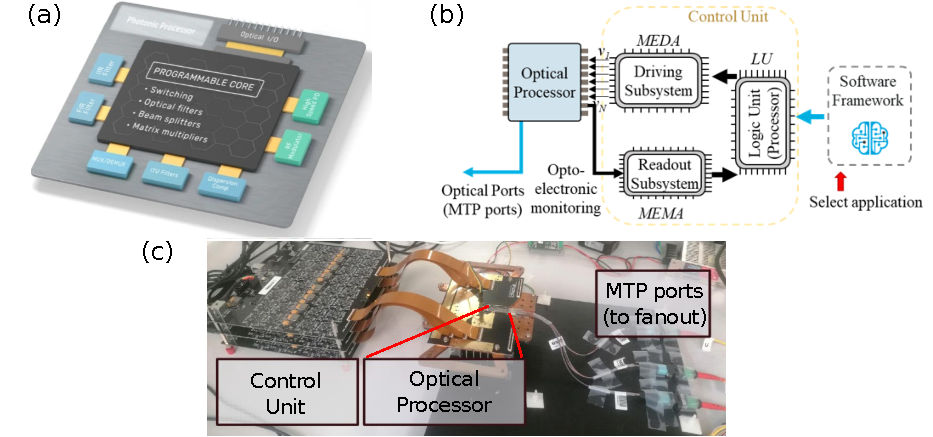
\includegraphics{figures/ch2-smart-subsystems.pdf}
	\end{center}
	\caption{(a) Optical layer of the processor with the core, I/Os, and high-performance blocks, (b) assembled chip with control unit and access fibers, (c) interconnection diagram between optical system, control unit and software layer.}
	\label{fig:ch2-smart-subsystems}
\end{figure}

Figure~\ref{fig:ch2-smart-subsystems} provides a glance of what is inside the first-generation Smartlight case.
In Fig.~\ref{fig:ch2-smart-subsystems}(a) we observe a diagram with the main block components of the reconfigurable photonic integrated circuit (PIC) with a core (dark gray) containing the reconfigurable PUC mesh which is connected through waveguides to high-performance blocks (HPBs).
The blue HPBs are pure optical circuits such as filters and multiplexers.
The green HPBs are RF optoelectronic components that enable microwave photonic applications.
All these subsystems enable the PIC to implement a wide range of applications such as filtering, splitting, switching, among others that will be covered in the next chapter.
Optical inputs/outputs (I/O) ports allow to-be-processed signals to flow in and out of the unit once the operation has been performed.
The chip is connected optically through a fiber array with 64 ports (see Fig.~\ref{fig:ch2-smart-subsystems}(c)), from which 28 are routed to the mesh core and serve as I/O ports while the rest are kept for internal testing.
These 64 PIC ports are distributed among the three MTP connectors at the front panel.
Additionally, the chip has been packaged electronically through wire bonding interconnection to a printed circuit board (PCB).
On the electronic layer, 304 on-chip phase actuators are controlled by a board-integrated programmable multichannel electronic driving array (MEDA) source connected to the logic unit (LU) (Fig.~\ref{fig:ch2-smart-subsystems}(c)).
Similarly, 40 on-chip photodetectors are measured through an on-board readout system connected to the logic unit.
This monitoring system is the so-called multichannel electronic monitoring array (MEMA) that provides feedback on the optical power at each mesh port and four HPBs (Fig.~\ref{fig:ch2-smart-subsystems}(c)).
Closing the workflow, the software running in the LU actuates over the photonic system and can get instant data of the circuit configuration.
The overall operation (set and readout times) is dominated by the driving unit, setting the reconfiguration time of the system to 15–90 ms.

\begin{figure}[h]
	\begin{center}
		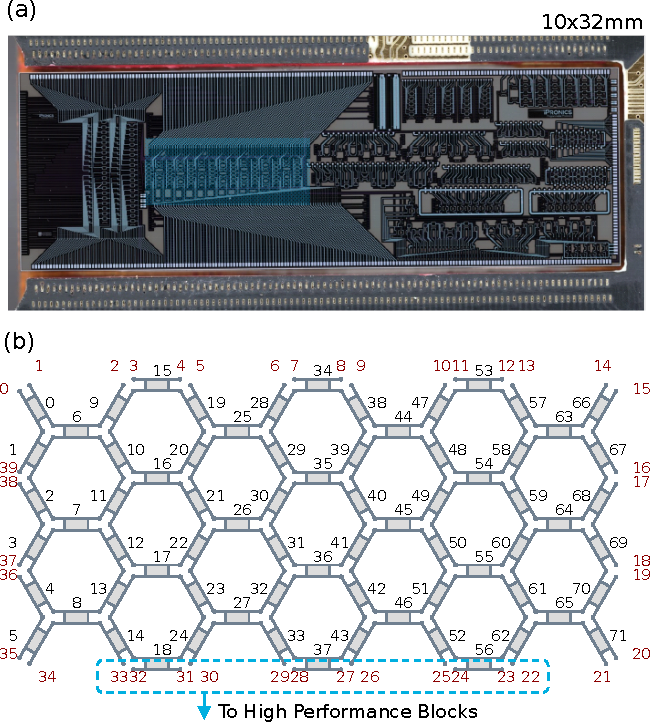
\includegraphics{figures/ch2-sw-smart-mesh.pdf}
	\end{center}
	\caption{(a) Picture of the chip with the highlighted region of the reconfigurable core, (b) schematic of the waveguide mesh core \cite{perez-lopez_general-purpose_2024}.}
	\label{fig:ch2-smart-mesh}
\end{figure}

The photonic stage is integrated into a silicon-on-insulator chip that includes a reconfigurable core of 72 Programmable Unit Cells (PUC) distributed in a flatted hexagonal mesh topology (see Figure~\ref{fig:ch2-smart-mesh}(a)) \cite{perez-lopez_general-purpose_2024}.
At the optical layer, the chip is optimized for C-band operation.
As described in Figure~\ref{fig:ch2-smart-mesh}(b), the mesh core has 40 output ports, 12 connected to on-chip HPBs (2 lattice filters of order 4, 1 coupled-ring filter, and 1 Ring-assisted MZI filter of order 4).
Further study and developments related to the HPBs lies beyond the scope of this thesis.
As described Sec.~\ref{sub:the_mach-zehnder-interferometer}, each PUC consists of a Mach-Zehnder Interferometer (MZI) with two thermo-optic phase actuators.
By tuning one of the arms, the user can modify the coupling factor of the 2-by-2 block.
For independent coupling factor and phase response configuration, the user/system can configure both arms.
The insertion loss and efficiency have been characterized across many chips and two wafers, resulting in 0.48 dB/PUC and 1.3 mW/π, respectively.
The basic unit length (BUL), i.e., the length of a PUC, and the basic unit delay (BUD), i.e., the signal delay during propagation through a PUC, are also characterized as 811 um and 11.25 ps, respectively.
Propagation losses are measured between 1.5 and 2.5 dB/cm for different waveguide widths and dies.
Finally, fiber-chip coupling loss ranges between 1.5 dB to 3 dB, for different coupling techniques.
For the scope of this paper, we employed a device with 3 dB loss per facet.
For further information, a detailed explanation of all the photonic specifications of first-generation Smartlight is provided in Table~\ref{tab:ch2-phot_specs}.

% \begin{noindent}
\begin{table}[ht!]
  \small
	\centering
	\begin{tabular}{|m{4cm}|m{1.0cm}|m{1.0cm}|m{1.0cm}|m{1.5cm}|m{5.5cm}|}
		\hline
		\multirow{2}{*}{\textbf{Specification}}         & \multicolumn{3}{c|}{\textbf{Value}} & \multirow{2}{*}{\textbf{Units}} & \multirow{2}{*}{\textbf{Description}}                                                                                                                                                                                                                                                                                                                              \\
		\cline{2-4}  % Line only below column 2 
		           & Min     & Typ.     & Max  &   &
		\\
		\hline
    Number of PUCs   &    & 72    &      & PUCs   & Arranged in the hexagonal lattice as shown in Figure~\ref{fig:ch2-smart-mesh}
		\\
		\hline
		Fiber to chip coupling loss/facet & 1.8  & <3.34 & 3.6  & dB & Fiber to chip coupling loss.
    \\
		\hline
		On-chip routing losses from and to optical I/Os & 5 & <7 & 8.4 & dB & On-chip routing losses from waveguides going into the mesh and coming out from it. 
    Facet loss not included.
		Mesh loss not included.
		\\
		\hline
		Losses per PUC  & 0.46  & 0.50  & 0.55  & dB   & 
    \\
		\hline
		Extinction ratio of PUCs & 32 & 35  & 44  & dB  & Difference between the maximum and minimum optical power obtained by sweeping a PUC's phase shifter. 
    Through port: 33 dB (Typ), Cross port: 44 dB (Typ).
		\\
		\hline
		30-dB isolation bandwidth of PUC & 30 & 45 & 65 & nm & Cross port: >60 (Median), Through port: 45 dB (Median).
		\\
		\hline
		±2\% Uniformity bandwidth & 3 & 5.5 & 15 & nm & Characterized for a coupling factor configuration of 50\%.
		Cross port: 8.1 ± 4.5 nm, Through port: 5.1 ± 1.55 nm.
		\\
		\hline
		Power consumption per phase shifter & 1.2 & 1.34 & 2.0 & mW/π  & 
		\\
		\hline
		Single-channel reconfiguration speed & & <14 &  & ms & <62.5 ms for 160 channels (writing).
		<0.3 ms for 50 channels (reading). 
    \\
		\hline
    Basic unit length (BUL) & & 811.41 &  & µm   & Length of a PUC. It sets the spatial resolution of the circuits programmed within the mes.
    \\
		\hline
    Basic unit delay (BUD) & & 11.25 &  & ps & Access path to the mesh accumulates 48 ps additionally.
		\\
		\hline
	\end{tabular}
  \caption{Optical specifications of a first-generation Smartlight unit.}
  \label{tab:ch2-phot_specs}
\end{table}
% \end{noindent}

% subsection  Optical Specifications (end)

% section Smartlight: The Field Programmable Photonic Gate Array (end)
\section{Software stack}\label{sec:software_stack}

\begin{figure}[h]
	\begin{center}
		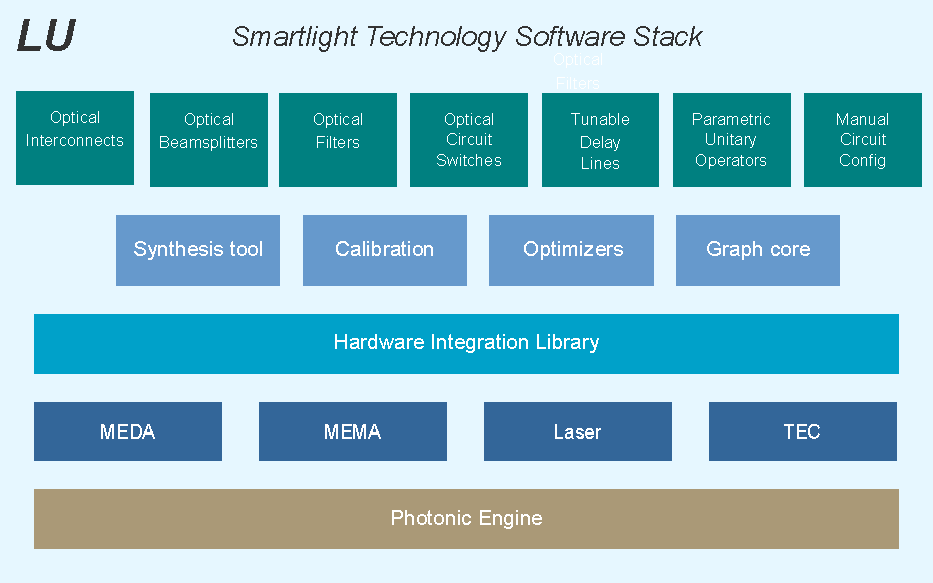
\includegraphics{figures/ch2-sw-stack.pdf}
	\end{center}
	\caption{Software stack developed under the framework of this thesis to control and operate on the reconfigurable PIC.}\label{fig:ch2-sw-stack}
\end{figure}

Programmable photonics involves a software framework that encompasses a wide array of algorithms, methods, or routines executed by a logic unit (LU) running a GNU/Linux distribution.
These serve primarily to configure specific functionalities within a Photonic Integrated Circuit (PIC) and to optimize the backplane.
These routines can be categorized based on their intended outcomes or their specific requirements as shown in Figure~\ref{fig:ch2-sw-stack}.
The first layer includes the low-level functions necessary to maintain the chip's temperature stable (TEC), drive (MEDA) and read (MEMA) from the photonic and electro-optic components, and control the tunable laser to feed signals into the system.
These subsystems of Smartlight are coordinated through the hardware integration layer that handles the calls to them and orchestrates the submodule communication.
On top of this layer sits a group of fundamental routines dedicated to enable high-level user functionalities and ensure the system's operation at an optimal point.
Among these we have PIC calibration routines (refer to Sec.~\ref{sub:calibration}), a set of finely tuned optimizers, a graph model of the PIC (see Sec.~\ref{sub:graph_layer}) and an elaborate synthesis tool that maps user configurations into low-level parameters to drive the photonic engine.
These modules often rely on calls to each other to yield observable outputs.
For instance, optimizer routines power the calibration of the electro-optical response of each phase shifter within the circuit, eliminating the need to integrate optical monitors into the waveguide mesh.
Additionally, these routines can extract valuable information such as the power consumption of individual units, accumulated losses to identify and record defects within the circuit.
The data collected can then be fed into a graph model to leverage on well-known network optimization algorithms, e.g., Dijkstra or A*, to optimize both the circuit's functionality and resource utilization.
The specific technical details of these software libraries will be presented in Chapter~\ref{chap:applications_using_fppgas}.
The same outcomes from the optimization, calibration and graph core utilities enable the manual and automatic synthesis of circuits in the first-generation Smartlight mesh.
The final layer exposes a Python API to the end users via the \lstinline|Smartlight| class which exposes the functionalities in Figure~\ref{fig:ch2-sw-calib} top layer.
This layer also includes a set of virtual scopes to monitor the status of the mesh configuration, the on-chip photodetector readings and a spectrum analyzer tool.
Examples of how to use these high-level methods and the monitors are presented in detail in Chapter~\ref{chap:applications_using_fppgas}.

\begin{figure}[h!]
	\begin{center}
		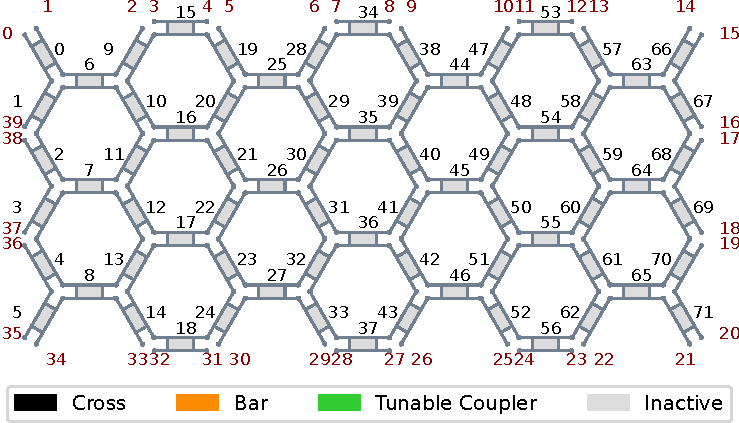
\includegraphics{figures/ch2-sw-mesh.pdf}
	\end{center}
	\caption{Representation of the first-generation Smartlight PIC hexagonal mesh developed during this thesis to monitor and track the status of the PUCs on demand.}\label{fig:ch2-sw-mesh}
\end{figure}

The latest Python API developed during this thesis is the \lstinline|iPronics_smartlight_v.1.12.1| which is compatible with Linux, macOS and Windows machines.
The software is tailored to work with the hexagonal mesh array presented in Section~\ref{sec:smartlight_fppga} of the iPronics first-generation Smartlight solution.
Although the higher layers in Figure~\ref{fig:ch2-sw-stack} are architecture agnostic, the lower levels are not.
The hardware integration layer has been developed to work with the MEDA, MEMA, TEC and laser subsystems inside Smartlight.
Nevertheless, the software infrastructure has been laid out in such a way that the inclusion of new peripherals (i.e., to favor version upgrades) can be performed without particular overheads.
Figure~\ref{fig:ch2-sw-mesh} depicts the output from the \lstinline|Core_Monitor| visualizer created to monitor the current status of the Smartlight photonic core.
Each PUC is represented as a rectangle with four ports (2 inputs and 2 outputs).
The label of each PUC is shown in black and the optical ports in red.
This monitor queries the MEDA registers to collect information about active PUCs in the system and plots it to the user using a color code system.
PUCs configured in cross, bar, coupler and inactive states are painted black, orange, green and gray, respectively.
Since this scope is showing the status of a mesh that has not been programmed, all PUCs are painted gray (i.e., inactive) which means that no control signal has been applied to their phase shifters which renders them at a random fabrication state.

\subsection{Calibration}\label{sub:calibration} % (fold)

\begin{figure}[h]
	\begin{center}
		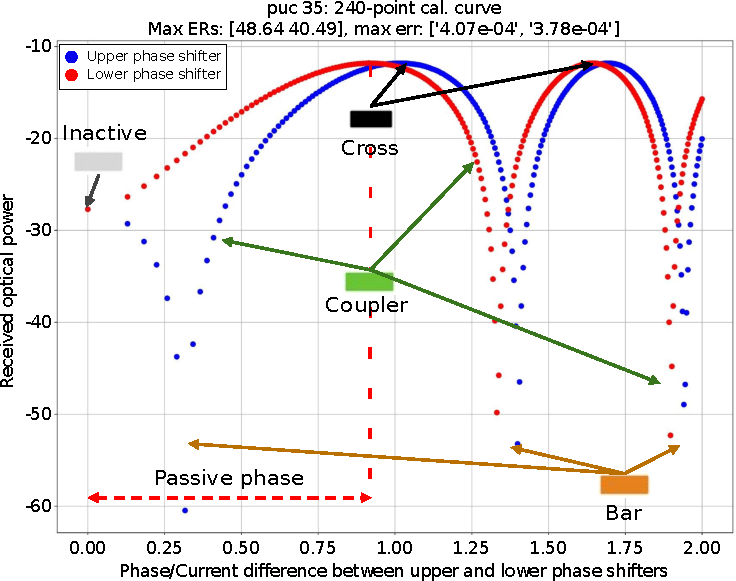
\includegraphics{figures/ch2-sw-calib.pdf}
	\end{center}
	\caption{Calibration trace of a PUC.
		Black/orange/green arrows point to the currents that set the cross/bar/coupler state of a PUC.
		These traces are essential to estimate the manufacturing passive phase of a PUC.
	}\label{fig:ch2-sw-calib}
\end{figure}

To program the Smartlight mesh effectively all PUCs must be calibrated previously, meaning that the electro-optic response of each phase shifter has been characterized and modelled correctly.
The calibration algorithm of a hexagonal mesh is an iterative process that relies on driving the phase actuators of the PUCs that form a path in the mesh until a set of currents that maximize the path's power has been found.
This set of currents corresponds to the biases needed to set these PUCs to cross and bar state, depending on the path of interest.
Once these points have been well-defined and set, the currents driving one PUC's phase shifters within the path can be swept to obtain their calibration traces as shown in Figure~\ref{fig:ch2-sw-calib}.
The calibration curves of a PUC's phase shifters provide details on the relationship between the applied current and the actual phase set by the actuator.
Fig.~\ref{fig:ch2-sw-calib} shows that, although the actuators should be at cross state by default (refer to Sec.~\ref{sub:the_mach-zehnder-interferometer}), they start at an intermediate point between bar and cross due to manufacturing errors.
The phase difference between the ideal cross state and the initial state is the so-called \textbf{passive phase}.
Since in this case the power is measured at the PUC's cross port, the maxima in these traces correspond to different cross-state currents in the 2\(\pi\) cycles.
Likewise, the minima correspond to the currents that set circuit to bar-state.
All the other currents between these previous points correspond to intermediate states that set the PUC as a tunable coupler (i.e., \(0 < k < 1\)).
The calibration routine of the first-generation Smartlight system allows setting \lstinline|k| values with a 0.001 resolution.
As presented in Eq.~\eqref{eq:ch2-phase_current}, the relationship between phase and driving current is non-linear, thus explaining why the cross and bar periods in Fig.~\ref{fig:ch2-sw-calib} get shorter for higher currents.

\begin{equation}
	\begin{aligned}
		\phi_{\text{up}} & = \rho_{2\_\text{up}} \cdot I^2 + \rho_{3\_\text{up}} \cdot I^3 + \alpha \\
		\phi_{\text{lo}} & = \rho_{2\_\text{lo}} \cdot I^2 + \rho_{3\_\text{lo}} \cdot I^3,
	\end{aligned}
	\label{eq:ch2-phase_current}
\end{equation}

where \(\phi\) corresponds to the phase applied by the actuator, \(\alpha\) is the passive phase and \(\rho_2\), \(\rho_3\) are the quadratic and cubic current-phase factors.
The last three parameters are the ones that must be identified for all phase actuators for the correct programming of circuits on the Smartlight mesh.
The full calibration routine involves creating several paths within the mesh, each with more PUCs than the previous one, so that over a number of iterations the calibration parameters of all phase actuators have been collected.
Further details about the calibration process can be found in \cite{lopez-hernandez_automatic_2022,jia_calibration_2024}.

% subsection Calibration (end)
\subsection{Circuit synthesis}\label{sub:circuit_synthesis} % (fold)

\begin{lstlisting}[caption={Manual synthesis of a basic circuit using the first-generation Smartlight API}, label=lst:ch2-sw-synthesis]
from smartlight import Smartlight
from smartlight.graphics import (
    CoreMonitor,
    MEMAMonitor,
    OpticalResponseVisualizer,
)
# Instantiate system
smart = Smartlight()
smart.set_input_port(0)
# Define circuit configuration
basic_circuit = [ (0, "x"), (6, "x"), (10, "x"), (16, "="), (20, "="), (19, "x") ]
smart.manual_circuit_configuration(basic_circuit)
# Monitor waveguide mesh
core_monitor = CoreMonitor(smart)
core_monitor.plot_mesh_status()
# Turn on laser
smart.enable_laser()
# Monitor on-chip PDs
mema_monitor = MEMAMonitor(smart)
mema_monitor.plot_current_mema_status()
\end{lstlisting}

The process to implement a basic circuit on the first-generation Smartlight mesh using the Python package developed during this thesis is exemplified in Listing~\ref{lst:ch2-sw-synthesis}.
The first step is to import the main libraries that enable user-device interaction.
\lstinline|Smartlight| represents the class that, once instantiated, boots Smartlight along all its subsystems.
\lstinline|CoreMonitor| is a virtual scope that monitors and tracks the PUC status in the mesh to enable circuit visualization (refer to Figure~\ref{fig:ch2-sw-mesh}).
\lstinline|MEMAMonitor| provides a power visualizer of on-chip photodetector readings (see Figure~\ref{fig:ch2-sw-synthesis}(b)).
\lstinline|OpticalResponseVisualizer| performs a laser sweep to capture the transmission spectral response of circuits configured on the mesh such as the ones in Section~\ref{sec:filters}.
Once the system has booted up, circuits can be implemented on it using the \lstinline|manual_circuit_configuration()| instruction which accepts a \lstinline|List(Tuple(puc_id, state))| to configure the mesh.
Where \lstinline|puc_id| corresponds to the PUC label as depicted in Figure~\ref{fig:ch2-sw-mesh} and \lstinline|state| can either be \lstinline|"x"| for cross, \lstinline|"="| for bar and \lstinline|k| (a floating-point number) for tunable coupler.

In Figure~\ref{fig:ch2-sw-synthesis} we observe the result of running Listing~\ref{lst:ch2-sw-synthesis} on a first-generation Smartlight system.
Figure~\ref{fig:ch2-sw-synthesis}(a) shows the \lstinline|CoreMonitor| output where we observe that all PUCs have been configured correctly to establish an optical path between ports 0 and 5.
Figure~\ref{fig:ch2-sw-synthesis}(b) contains the \lstinline|MEMAMonitor| output for this circuit which, as expected, has routed most of the optical power from input 0 to the photodetector connected to port 5.

\begin{figure}[h]
	\begin{center}
		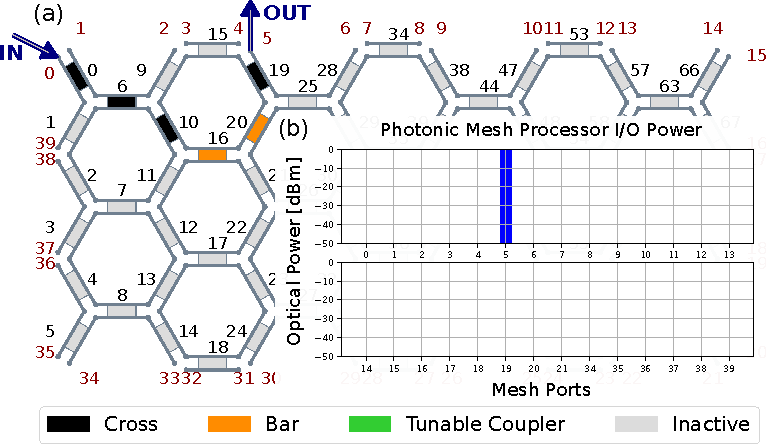
\includegraphics{figures/ch2-sw-synthesis.pdf}
	\end{center}
	\caption{Basic interconnect circuit synthesized using manual configuration.
		Individual PUC states are defined using 'x', '=' or 'k' states.
	}\label{fig:ch2-sw-synthesis}
\end{figure}

An additional method to configure circuits on the mesh is \lstinline|set_coupling_factor_phase()| which allows setting not only the coupling factor \(k\) but also the cross-phase \(\Delta\) (refer to Section~\ref{sub:the_mach-zehnder-interferometer}) of each individual PUC.
The \lstinline|set_coupling_factor_phase()| accepts as arguments a \lstinline|List(Tuple(puc_id, List(state, cross_phase)))| where \lstinline|cross_phase| corresponds to the PUC's common transmission phase in radians, and the rest of parameters remain the same as described above.
This functionality provides the end-user with very precise control over the amplitude and phase of the synthesized circuits.
Practical examples of how this instruction can be the key enabler of certain phase-sensitive applications are presented in Chapter~\ref{chap:applications_using_fppgas}.

% subsection Circuit synthesis (end)
\subsection{Graph layer}\label{sub:graph_layer}

To control the photonic processor, a software layer based on graphs is used.
Graph theory \cite{kerchove_automated_2023} provides a framework for analyzing and solving problems related to connectivity, paths, cycles, and other properties of graphs.
A graph model representing the mesh in the first-generation Smartlight system has been developed and is integrated with the product.
In the latter, all the connectivity and topology of hexagonal mesh can be abstracted into a model, in which the optical ports of the PUCs are represented as nodes in the graph, and the flow of light in the waveguides can then be represented by edges connecting these nodes.
One challenge in graph representation of hexagonal mesh is the feedback loops in the circuit.
To address this, we chose the directed graph with eight artificial nodes \cite{chen_graph_2020} for our model, where each port of PUC is represented with two artificial nodes, for inbound and outbound of the signal.
Specific details of the graph implementation are provided in reference \cite{xie_software-defined_2024}.
The PUC phase shifters are modeled by arcs with the direction of input and output ports.
The graph representation incorporates performance metrics for each connection, which means each arc is assigned a weight as expressed by Equation~\eqref{eq:ch2-graph_weight} where IL is the PUC insertion loss, BUL is the PUC basic unit length, and P is the PUC's power consumption.

\begin{equation}
	w = c_1 \cdot \textit{IL} + c_2 \cdot \textit{BUL} + c_3 \cdot P + \dots
	\label{eq:ch2-graph_weight}
\end{equation}

Hence, the weight can be calculated according to these figures of merit (FOM) by only changing the distribution of weights \(c_i\) \cite{lopez_auto-routing_2020}.
The underlying graph layer in the Smartlight API is one of its most powerful libraries as it powers several applications and allows defining circuit implementations that optimize insertion losses, power consumption and other non-ideal effects automatically.
The auto-routing algorithm powered by this graph model assumes a critical role in this process, as it automatically determines optical paths and interferometric structures within the waveguide mesh topology.
Furthermore, the latter routine introduces groundbreaking self-healing and fault-tolerant capabilities for the PIC.
When confronted with damaged areas within the mesh, the algorithm is adept at identifying alternative suboptimal paths to be used by circuits.

% subsection Graph layer (end)
\subsection{Automatic synthesis}\label{sub:automatic_synthesis} % (fold)

\begin{lstlisting}[caption={Automatic synthesis of a basic circuit using the first-generation Smartlight API}, label=lst:ch2-sw-auto-synthesis]
	# Automatic configuration
	PUCs_configuration = smart.interconnect_auto(input_port=0, output_port=6)
	\end{lstlisting}

Automatic synthesis involves selecting and arranging PUCs in a manner that automatically defines the paths taken by the optical signal fed into the chip.
For a given specification, such as achieving a 10 ns delay between two specific optical ports, multiple solutions may exist.
In this context, a software layer powered by a graph model is capable of determining the configuration solutions that minimize the number of PUCs required, the driving power, etc. depending on the FOM to optimize by the solution of interest.
With a graph model at hand we can leverage on ubiquitous, yet extremely influential, algorithms such as Dijkstra/A* \cite{bierlaire_optimization_2015} and network optimizers to facilitate the convergence on optimal circuit configurations, as evidenced by references \cite{lopez_auto-routing_2020,perez-lopez_multipurpose_2020}.
The resultant configurations can be stored for future use and employed to dynamically configure the circuit.
Listing~\ref{lst:ch2-sw-auto-synthesis} shows the example of how to implement the interconnect circuit defined in Listing~\ref{lst:ch2-sw-synthesis} using an automatic instruction based on the graph layer presented previously.
Note that now there's no need to define the individual states of the PUCs as they are returned and configured by the \lstinline{interconnect_auto} instruction.
In this particular case the resulting mesh configuration is the same one presented in Figure~\ref{fig:ch2-sw-synthesis}.
An extensive set of examples of how to perform automatic synthesis of several applications and their implementation details are presented in Chapters~\ref{chap:applications_using_fppgas} and \ref{chap:universal_unitary_operators}.

% subsection Automatic synthesis (end)
% section Software stack (end)


% Author: David Sanchez-Jacome

\chapter{Applications using FPPGAs}\label{chap:applications_using_fppgas} % (fold)

The emergence of the field programmable photonic gate array (FPPGA) platform, presented in the prior chapter, powered by a high-level software layer unlocks the door to a wide set of applications.
The Python API layer developed during this thesis enables the users of the platform to synthesize several types of circuits in the mesh where the PUCs can either be configured in cross, bar or tunable coupler states.
We recall that since the PUCs have two drivable arms their coupling factor and cross-phase can be set independently (as covered in Section~\ref{sec:software_stack}), allowing us to expand the flexibility of the configured circuits.
In this chapter we present a set of applications demonstrated on the first-generation Smartlight platform by our team and in collaboration with other research centers around the world.
The chapter puts emphasis on presenting the Python code used to configure and measure these circuits, enabling interested readers to reproduce them using either the hardware platform or the system simulator.

\section{Interconnects}\label{sec:interconnects} % (fold)

\begin{lstlisting}[caption={Implementation of manual and automatic interconnects using the first-generation Smartlight API}, label=lst:ch3-interconnects]
	# Manual configuration
	puc_info = [
		(0, "x"),
		(6, "x"),
		(10, "x"),
		(16, "="),
		(20, "x"),
		(25, "x"),
		(28, "="),
	]
	smart.interconnect(puc_info)
	# Automatic configuration
	PUCs_configuration = smart.interconnect_auto(input_port=0, output_port=6)
	\end{lstlisting}

Reconfigurable optical interconnects are of great interest in optical networks as they enable flexible connections of terabit data rates with high-performance operation \cite{khani_sip-ml_2021}.
These interconnects demand reduced latency and energy efficiency between input and output (I/O) ports, and therefore minimal insertion loss and shortest distance is highly desired.
These circuits are the simplest and can be implemented by manually setting the PUCs to cross and bar states.
This can be done by passing the API a dictionary-like structure specifying the individual states of each PUC.
Additionally, the graph layer presented in Section~\ref{sub:graph_layer} provides an interconnect algorithm based on Dijkstra \cite{foead_systematic_2021,bierlaire_optimization_2015}, which can automatically provide an optimum path configuration.
This automatic implementation can also provide self-healing capabilities to allocate alternative optical paths with lower insertion loss when needed.
The manual and automatic code implementations are presented in Listing~\ref{lst:ch3-interconnects}.

\begin{figure}[h!]
	\begin{center}
		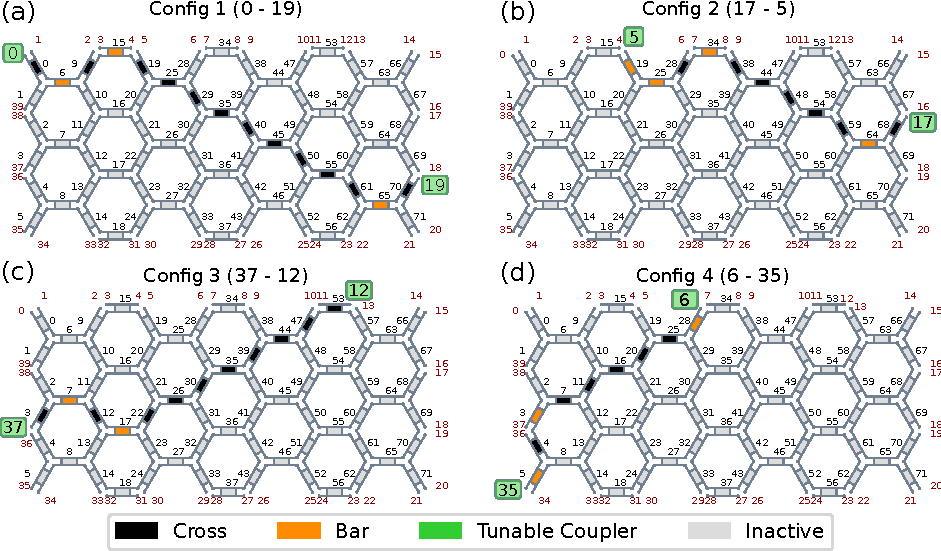
\includegraphics{figures/ch3-interconnects.pdf}
	\end{center}
	\caption{Optical interconnect experiment.
		Programmable path configurations considering different input ports.
	}\label{fig:ch3-interconnects}
\end{figure}

\begin{figure}[t]
	\begin{center}
		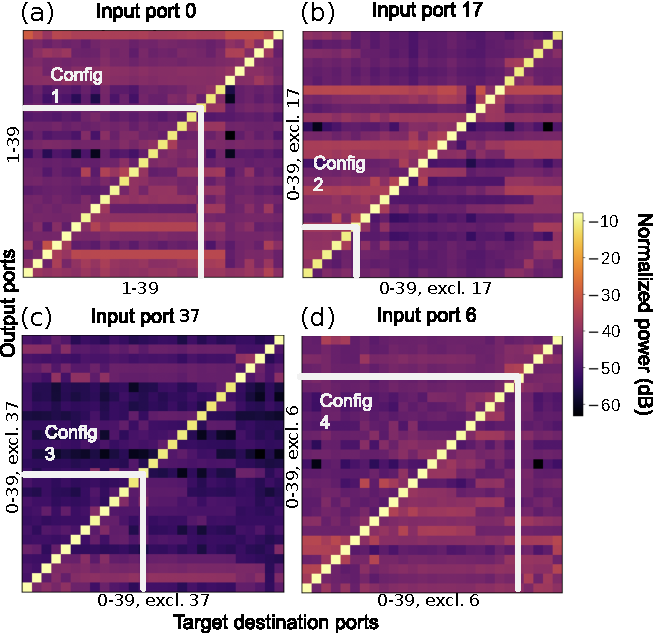
\includegraphics{figures/ch3-inter_power_meter.pdf}
	\end{center}
	\caption{Optical interconnect experiment.
		Colormap of the optical power measured at output ports for different interconnect configurations normalized to the laser input power (5~dBm).
		The white lines indicate the configuration shown in the schematic of the programmable processor.
		The HPB ports [22-33] are not considered as they are neither routed to a PD nor exit the PIC.
	}\label{fig:ch3-inter_power_meter}
\end{figure}

The results of the optical interconnect experiments at a central wavelength of 1550 nm and the processor configurations are shown in Figure~\ref{fig:ch3-interconnects}.
Ports 0, 17, 37 and 6 are used as input ports, and up to 27 interconnects to other available output ports are programmed as the HPB ports [22-33] can't be used as output ports since they are neither routed to a PD nor exit the PIC.
As it can be seen in Figure~\ref{fig:ch3-inter_power_meter}, all the paths are configured successfully, showing diagonal lines in the colormap, each one corresponding to a given interconnect.
The power of the measured output is normalized to the input power of the laser (5 dBm).
The insertion loss at each target port is between 7.7 dB and 10.5 dB, depending on the number of PUCs used to configure the path.
In the experiment, the longest interconnect path consists of 15 PUCs, while the shortest is only 2 PUCs which produces a certain power imbalance between outputs related directly to the losses per PUC (\(\approx\)0.46 dB).
Furthermore, optical power is also measured at the rest of the non-targeted output ports, with an average leakage of -30 dB.
The algorithm allows the simultaneous identification of up to 400 possible paths with an average time of about 0.4 microseconds per path.
% section Interconnects (end)

\section{Beamsplitters}\label{sec:beam_splitters} % (fold)

\begin{figure}
	\begin{center}
		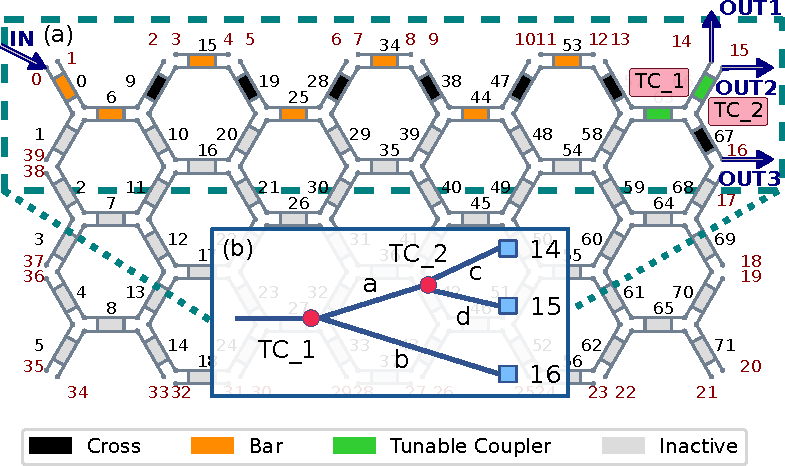
\includegraphics{figures/ch3-splitter.pdf}
	\end{center}
	\caption{Optical beam splitting demonstration: The first-generation Smartlight programmable processor synthesizing a 1x3 splitter configuration.
		The inset shows the detailed graph.
	}\label{fig:ch3-splitter}
\end{figure}

Optical beam splitting allows for a single optical signal to be efficiently distributed across multiple receiving nodes or devices simultaneously.
This is particularly advantageous in scenarios where the same data needs to be delivered to several destinations within a data center cluster, simultaneously.
This functionality is currently not available in the physical layer of most networks.
So, if deployed under the right software stack support it has the potential to open the door to new, cost-efficient and disruptive applications.
One added advantage brought in by PIP is the software-defined control of the splitting ratio across the outgoing signals powered by the fine-tuning of driving phases applied to the PUCs.
As a consequence of this, the operator can then control how much power is allocated to different receiving nodes in a dynamic manner.

Beamsplitter circuits can be implemented manually on the first-generation Smartlight platform similarly to the interconnects presented in the previous section.
In this case however, the state of some PUCs can be set to a floating-point value corresponding to the splitting factors required by the circuit.
A simple example of a 1-by-3 network is demonstrated in Figure~\ref{fig:ch3-splitter}.
The graph representation of the beamsplitter network is useful when determining how the splitting circuit can be mapped on the hexagonal mesh as presented in Fig.~\ref{fig:ch3-splitter}.
In Listing~\ref{lst:ch3-splitter} we define such beamsplitter which uses 0 as input port and ports 14, 15 and 16 as outputs.
The optical splitting happens in PUCs 63 and 66 where the coupling factor is set to 1/3 and 2/3, respectively.
This splits the optical power equally among the three outputs.
The coupling factors of the other PUCs take the value '=' or 'x', which corresponds to bar state (k = 0) or cross state (k = 1).

Additionally, in this work, we have designed an auto-beamsplitter algorithm that can accommodate any number of desired outputs from a given input.
It determines the optimum path to each output, and efficiently autoconfigures the splitting PUCs with a ratio that ensures every output port receives the same power, for a traditional beamsplitter operation, or the specified power ratio, under custom operation \cite{xie_software-defined_2024}.
To achieve this, the auto-beamsplitter algorithm can be translated into a single-source shortest path problem represented by a directed acyclic graph (directed tree) \cite{perez-lopez_programmable_2018}.
As observed in Listing~\ref{lst:ch3-splitter}, the auto-beamsplitter allows the user to define a beamsplitter from the given input and outputs ports, and this functionality will find the specific PUCs to be used and define their coupling factors.
The optimal path will be selected based on the FOM that we defined in Section~\ref{sub:graph_layer}.

\begin{lstlisting}[caption={Implementation of manual and automatic beamsplitters using the first-generation Smartlight API}, label=lst:ch3-splitter]
# Manual configuration
puc_info = [
    (0, "x"), (6, "="), (9, "x"), (15, "="), (19, "x"), (25, "="),
    (28, "x"), (34, "="), (38, "x"), (44, "="), (47, "x"),
    (53, "="), (57, "x"), (63, 1/3), (66, 2/3), (67, "x"),
]
smart.beam_splitter(puc_info)
# Automatic configuration
pucs_configuration = smart.beam_splitter_auto(input_port=0, output_ports= [14,15,16]) 
\end{lstlisting}

When light is divided at a TC it will traverse two different paths, defined here as cross and bar paths, until it reaches the output ports.
The inherent insertion loss difference between these paths will cause an undesired power imbalance at the outputs, i.e., the power ratio between the outputs will not be as intended.
Therefore, it is vital to account for the insertion losses in both paths (cross and bar) coming out of a TC and compensate them to achieve the targeted power distribution, see Eq.~\eqref{eq:ch3-k_nonideal}:

\begin{equation}
	k = \frac{k_T}{(1 - k_T) \cdot 10^{\frac{IL_b - IL_c}{10}} + k_T}
	\label{eq:ch3-k_nonideal}
\end{equation}

where \(k_T\) is the ideal splitting ratio of the tunable coupler PUC, and \(IL_b\) and \(IL_c\) are the bar path and cross paths' insertion losses, respectively.
For the paths that contain a leaf node, such as edge c, d, and b in Figure~\ref{fig:ch3-splitter}, their insertion losses can be calculated with the following equation:

\begin{equation}
	IL_{edge} = \sum IL_{PUC} \label{eq:ch3-il_leaf} \end{equation}

where \(IL_{PUC}\) is the insertion loss of all the PUCs in that particular path.
On the other hand, for the insertion losses of a branch (path) that contains a child node, such as a path a leading to the $TC_2$ subtree in Figure~\ref{fig:ch3-splitter}, the paths’ insertion loss of $TC_1$ can be calculated with \eqref{eq:ch3-il_parent}.

\begin{equation}
	IL_{cross(bar)} = 10 \cdot \log \left( k_q \right) + IL_{q,cross} + IL_{path} \label{eq:ch3-il_parent} \end{equation}

In the latter, \(k_q\) represents the coupling factor of the child node $q$ (in this case $TC_2$), \(IL_q\), is the insertion loss of child node $q$ in the cross path, and \(IL_{path}\) is the insertion loss between the parent node and the child node \cite{perez-lopez_programmable_2018}.

In this demonstration, we showcase the beamsplitter capabilities of our programmable processor driven by our control software layer.
Specifically, we have implemented a 1-by-26 on-chip splitter circuit.
Port 0, connected to a 5 dBm source, serves as input while the rest of ports act as receiving nodes.
The result has been normalized with respect to the input power and measured at a central wavelength of 1550 nm, see Fig.~\ref{fig:ch3-splitters_power_meter}.
Our experimental approach began with a 1-by-1 circuit and progressively expanded the number of output ports up to 26.
For each configuration, we have recorded the powers at all output ports and have placed them as columns of the results' matrix in Fig.~\ref{fig:ch3-splitters_power_meter}, so that the first and last columns represent the outgoing power distribution for the 1-by-1 and 1-by-26 cases, respectively.
The resulting visualization of output power distribution versus number of receiving nodes exhibits a horizontal funnel pattern and demonstrates how evenly the signal can be shared across the chip ports.
The yellow area systematically expands from the left side to the right, while the color tone changes to orange.
This trend indicates that with an increasing number of ports, the power allocated to each port decreases, up to a minimum of -22 dB in the 1-by-26 case.
Notably, the power intensity across all configured output ports remains uniform.
Fig.~\ref{fig:ch3-splitters_power_meter}(b) offers another perspective to the power splitting feature, here we demonstrate that the average power exhibits a logarithmic decrease as the number of ports increases.
The deviation shows a gradual increase with the number of targets: The minimum deviation is 0.663 dB, and the maximum is 1.31 dB for 1-by-2 and 1-by-26 beam splitting, respectively.
This increase in deviation is a consequence of the coupling factor dependence on the cross and bar insertion losses of the outgoing paths as shown in Eq.~\eqref{eq:ch3-k_nonideal} The latter entails that in order to have an accurate compensation of path loss difference we require a precise measurement of each PUC’s insertion loss.
However, for this work we have relied on an average loss value for all the PUCs, therefore, as more of these are added to the circuit, more deviation is expected.
In addition to path loss difference errors, optical crosstalk originating from a PUC can also contribute to non-uniform output powers.
In the chip platform used in this work, we have measured that the optical crosstalk of individual PUCs is always below -25 dB.
Note that we could also employ the on-chip photodetectors and the closed feedback loop to dynamically adjust or fine tune the coupling factors to correct all aforementioned errors starting from the analytical seed provided by the presented algorithm \cite{perez-lopez_multipurpose_2020}.

\begin{figure}
	\begin{center}
		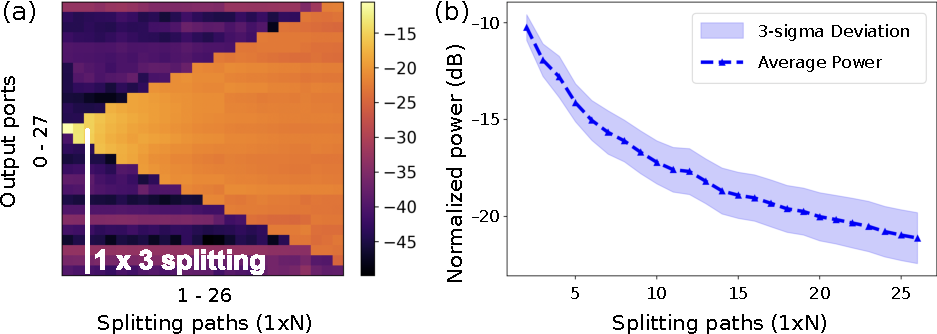
\includegraphics{figures/ch3-splitters_power_meter.pdf}
	\end{center}
	\caption{Optical beamsplitter demonstration: (a) Output power colormap as a function of
		the number of splitting paths starting from 2 (second leftmost column) and 26 (rightmost column).
		The white lines point to the measured output powers for the configuration in Fig.~\ref{fig:ch3-splitter}.
		We observe how the input laser power is evenly distributed across the output ports.
		In (b) we observe the average output power and its deviation with respect to the number of splitting paths.
	}\label{fig:ch3-splitters_power_meter}
\end{figure}

% section Beam splitters (end)

\section{Switches}\label{sec:switches} % (fold)

\begin{figure}
	\begin{center}
		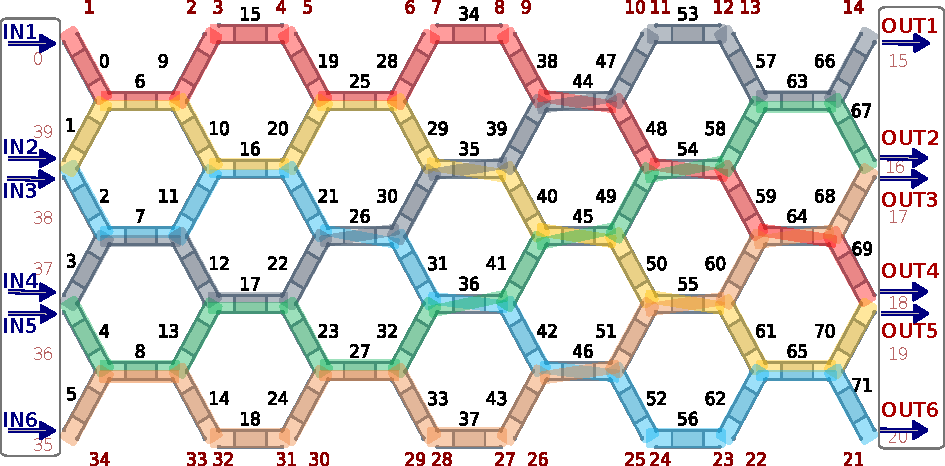
\includegraphics{figures/ch3-ocs.pdf}
	\end{center}
	\caption{Optical circuit switching experiment.
		Programmable processor 6x6 circuit switch configuration.
		Input ports 0, 39, 38, 37, 36, 35 and output ports 15, 16, 17, 18, 19, 20 are numbered from 1 to 6 each in blue color and red color respectively.
	}\label{fig:ch3-ocs}
\end{figure}

Optical circuit switching is a technology that allows to configure the physical layer of an optical network through software instructions.
It holds the potential to improve the cost, latency and power consumption used by ML/AI workloads within data centers \cite{khani_sip-ml_2021,liu_lightwave_2023,sato_prospects_2022}.
When the traffic circulating in a network is deterministic the physical layer can be used to route the data directly and the need for an Electronic Packet Switch (EPS) can be avoided.
In this section, we present the implementation of an on-chip software-defined switch that enables the dynamic control of optical waveguide paths for multiple input and output channels.
Such a system has been synthesized on the hexagonal core introduced previously and has been designed to cross-connect 6 pairs of inputs-outputs.
To enable the automatic configurability of the full 6-by-6 switch matrix we have adapted three algorithms and implemented them in our software stack.
The algorithms explored in this work are sequential routing \cite{lopez_auto-routing_2020}, graph-based with edge weight penalty \cite{kerchove_automated_2023}, and analytical decomposition \cite{jia_six-port_2018}.
The first two are more general as they make use of iterative algorithms to find the non-conflicting routes between the set of port pairs.
The first is the most time-consuming of the three as it relies on testing all possible I/O port routes until it finds a non-conflicting solution.
The edge penalty approach is an iterative algorithm that makes use of dynamic weight updates in the graph to penalize conflicting path sections.
Once the weight is updated the routine will attempt to find a new route in the next iteration.
The \lstinline|max_iter| parameter (see Listing~\ref{lst:ch3-ocs}) regulates the maximum number of iterations for path re-routing in instances of edge conflicts, when no routing solution exists for certain input/output port combinations.
The third approach is fully analytical and relies on the mathematical decomposition of the switch matrix to a Spanke-Bennes network synthesized on the hexagonal mesh.
The solution in this case is immediate due to the analytical nature of the problem, however, the set of hexagonal core ports that can be used are restricted by the feed-forward network architecture.
The latter statement means that only the ports on the west and east side of the mesh can be used by this method, whereas the north and south ports can only be included for the iterative ones.
Regarding switching speed, the device's reconfiguration time is primarily determined by the thermo-optic actuator, which operates on the scale of microseconds, compared to hundreds of milliseconds in the case of MEMs-based approaches \cite{poutievski_jupiter_2022,urata_mission_2022}.

\begin{lstlisting}[caption={Implementation of iterative and analytical switch networks using the first-generation Smartlight API}, label=lst:ch3-ocs]
# Iterative method
input_ports = [0, 1, 2, 3, 4, 5]
output_ports = [5, 1, 2, 3, 4, 0]
pucs_configuration = smart.auto_switch(
    input_ports, output_ports, max_iter=50 
)
# Analytical method
switch_config = {0: 5, 1: 1, 2: 2, 3: 3, 4: 4, 5: 0}
feedforward = smart.feedforward_operator(dim=6, puc_0=0)
feedforward.load_switch_config(switch_config)
smart.load_feedforward_config(feedforward)
\end{lstlisting}

The first and third approaches are straightforward to implement and have been previously documented \cite{lopez_auto-routing_2020,jia_six-port_2018}.
The second approach was developed by iPronics and is detailed in depth in \cite{xie_software-defined_2024}.
The edge penalty algorithm has the advantage of being more efficient than the brute force algorithm (first approach) and more flexible than the third as it is not constrained to the ports of a Spanke-Bennes network.
Refer to Listing~\ref{lst:ch3-ocs} for the implementation of a 6-by-6 switching network using the iterative and analytical approaches, respectively.
The iterative one implements the weight-penalty/re-routing algorithms while the analytical method relies on the Clements decomposition of unitary switch matrix operators which will be covered in detail in Chapter~\ref{chap:universal_unitary_operators}.
% In lines 1 and 2, the best paths for each I/O port pair are identified.
% The next step is to check whether these paths contain conflict edges (line 4), as conflicting edges within the identified paths will be penalized with a higher weight (line 6).
The iterative method relies on identifying conflicting edges within a switch network and finding alternative paths to circumvent the conflicting zones.
What we define as a conflicting edge is a PUC that belongs to two or more paths and has a different state (cross/bar) in at least two of these paths.
A switching network needs to have zero conflicting edges to work.
% Once the problematic edges have been penalized, we recompute new optimal paths for the I/O ports pairs considering the new edge weights and updating the preprocessing paths configuration list (line 7, 8).
The algorithms iterate until the conflicts across the network have been solved.
If no conflicts are detected, the configuration of optimal paths will be saved and the loop will be stopped, otherwise the iterative process of weight update will continue until a zero-conflict configuration is found or the max number of iterations is reached.
If the number of iterations goes beyond the \lstinline|max_iter| value, the problem will be considered unsolved.
Hence, this variable represents the trade-off between the probability of finding a solution and the time spent searching for a zero-conflict configuration.
As mentioned before, the analytical method ensures the existence of a solution under the condition that only the input/output ports of a feedforward operator (e.g., the ones in blue/red in Fig.~\ref{fig:ch3-ocs} for an operator of size $N=6$) are used.
The rest of the hexagonal mesh ports would remain idle.
As stated previously, if there's a need to use other hexagonal mesh ports then the iterative algorithms are the ones to go with.
This particular case might be useful for some testing/prototyping applications that require additional flexibility.

In Figure~\ref{fig:ch3-ocs} we present the implementation of a 6x6 optical circuit switch with the different paths painted in different colors and all PUCs activated.
Notice that we have selected six ports from the left side of the hexagonal mesh [0, 27, 26, 25, 24, 23] as inputs and other six ports from the right side [15, 16, 17, 18, 19, 20] as outputs, the selected ports from both sides are named from 1 to 6 in blue color and red color, respectively.
To measure the performance of the network, six distinct switch configurations have been implemented using a laser source with 5 dBm input power connected to port 1.
The switch was then programmed to synthesize 6 different configurations between this input and all the possible outputs.
With the network defined, the power of each output port was measured and normalized with the input source, resulting in the characterization of 6 switch matrices.
The process was repeated for the other 5 inputs leading to the characterization of 36 switch matrices in total.
We denote that due to limited lab equipment at the time we characterized the switch by looking one input port at a time.
This means that, when all input ports are populated the total optical crosstalk will be slightly higher than the reported value (\(\approx [22,25]\) dB).
Nevertheless, later trials with six laser signals confirm that the 6-to-6 switch correct functioning holds \cite{sanchez-jacome_parametric_2024}.

In Figure~\ref{fig:ch3-ocs_power_meter} we present the measured results.
Here, each column in the subfigure represents the optical power monitored in a specific output port, and the different marker shapes correspond to the 6 different input ports.
Our results demonstrate the optical circuit switch’s performance showcasing accurate switching of multiple inputs to their respective target outputs.
Notably, the distances of all switch circuit paths are consistent, passing through 15 PUCs.
As a result, we observed -10 dB (± 0.5) insertion losses in all 6 output ports for each configuration.
The Attenuation-to-crosstalk ratio (ACR) is determined by checking the difference between the optical power from the specified input output pair and the highest leakage power from other input ports to the same output port.
This distinction is visually represented by the distance between two blue lines in Fig.~\ref{fig:ch3-ocs_power_meter}, with a typical value of 25 dB.
This metric varies based on the switch configuration, the best scenario of crosstalk observed in our experiments is 26 dB for the switch configuration: [1:4, 2:5, 3:6, 4:1, 5:2, 6:3].
The source of crosstalk is mainly from PUC performance, as well as small drifts due to auto-calibration and auto-characterization.
% ===Leaving reconf time out to avoid having conflicts of interest with iPronics ===
% The reconfiguration speed can be broken down in physical layer reconfiguration, control plane latency and algorithm computation time as shown in Table 2.
% Physical layer latency independent of number of elements to be tuned but control plane scaling linearly with number of PUCs.
% Software plane time ranges from milliseconds to seconds based on algorithm choice, in which edge penalty and sequential routing approaches take more time as they require a conflict-edge resolution step.

% Table 2.
% Configuration speed of optical switch circuit
%
% Latency (ms) Physical layer 0.18 Control plane 48 Algorithm Computation 38 (1) 2700 (2) 5800 (3) Total 86.18 (1) 2748.18 (2) 5848.18 (3)
%
% (1) Analytical decomposition.
% (2) Edge penalty algorithm. (3) Sequential routing
% ===Leaving reconf time out to avoid having conflicts of interest with iPronics ===

Using the same set of selected I/O ports, we evaluate the feasibility of the algorithm.
For the 6x6 circuit switch, there are a total of \(6!
=720\) possible combinations, representing distinct switch circuits for both, iterative and analytical algorithms.
The switching architecture can be classified as rearrangeable non-blocking as it needs to reconfigure already established connections to allocate new ones.
The algorithm demonstrated its reliability by generating feasible solutions for all 720 cases without any observed instances of failure.
This fact makes the software layer developed for this work a key differentiator with respect to previous manually implemented solutions.

\begin{figure}
	\begin{center}
		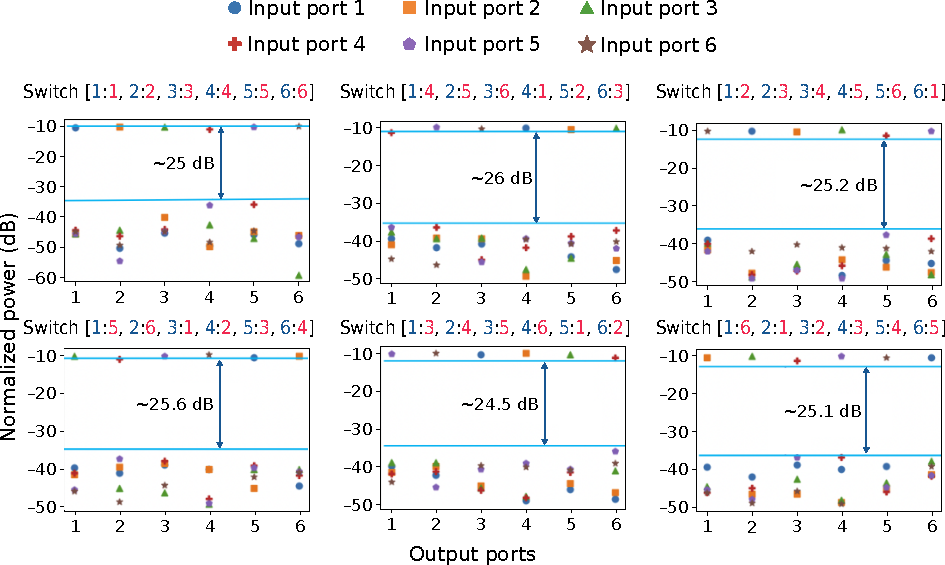
\includegraphics{figures/ch3-ocs_power_meter.pdf}
	\end{center}
	\caption{Optical circuit switching demonstration:
		6-by-6 switch matrix for 6 different configurations.
		Each subplot demonstrates the output of a specific switch configuration, with the X-axis depicting the output ports in the mesh and the Y-axis representing the measured optical power levels at the output ports.
		The six input ports are visually represented by six distinct markers in the figure.
	}\label{fig:ch3-ocs_power_meter}
\end{figure}

% section Switches (end)

\section{Filters}\label{sec:filters} % (fold)

% Tunable and reconfigurable photonic filters
The first-generation Smartlight photonic processor has the ability to implement various types of tunable and reconfigurable photonic filters.
These filters are crucial for microwave photonics (MWP) applications, as they allow precise signal shaping, noise reduction, and channel selection in the radiofrequency (RF) domain \cite{marpaung_si3n4_2013,liu_integrated_2020,daulay_tutorial_2021}.
In traditional systems, photonic filters are fixed-function devices or require bulky, discrete optical components.
The programmable photonic processor overcomes these limitations by offering on-chip tunable filters, implemented through software-controlled photonic circuits.
This platform can implement multiple types of tunable filters, including finite impulse response (FIR) filters such as unbalanced Mach-Zehnder interferometers (UMZIs) and lattice filters.
The same applies to infinite impulse response (IIR) such as optical ring resonators (ORRs), ring-assisted Mach-Zehnder Interferometer (RAMZI) filters, coupled resonant waveguide (CROW) filters, side-coupled integrated spaced sequence of optical resonators (SCISSORS) of multiple orders.
These filters are realized through the hexagonal waveguide mesh with 72 PUCs and the filter's order is limited by this core size.

\begin{lstlisting}[caption={Implementation of IIR and FIR optical filters using the first-generation Smartlight API}, label=lst:ch3-filters]
# IIR Filter 
smart.reset_mesh()
# 3rd order CROW
crow = [
    (1, "="), (2, k1), (6, "="), (7, "="), (9, "="), (10, k2),
    (11, "="), (15, "="), (16, "="), (19, "="), (20, k3),
    (21, "="), (25, "="), (26, "="), (28, "x"), (29, k4),
    (30, "="),
]
# 2nd order:
# [(28, "x")], 25 -> inactive
# FIR Filter 
smart.reset_mesh()
lattice = [
    (1, "="), (2, "x"), (3, k5), (6, "="), (7, "x"), (10, "x"),
    (11, "x"), (16, k6), (20, "x"), (21, "x"), (25, "="),
    (26, "x"), (29, "="), (30, "x"), (31, k7), (32, "x"),
    (33, "="), (36, "x"), (37, "="), (42, "x"), (43, "x"),
    (46, k8), (47, "x"), (48, "x"), (49, "x"), (50, "x"),
    (51, "="),
]
puc_info = crow # lattice 
smart.filter(puc_info)
\end{lstlisting}

\begin{figure}[t!]
	\begin{center}
		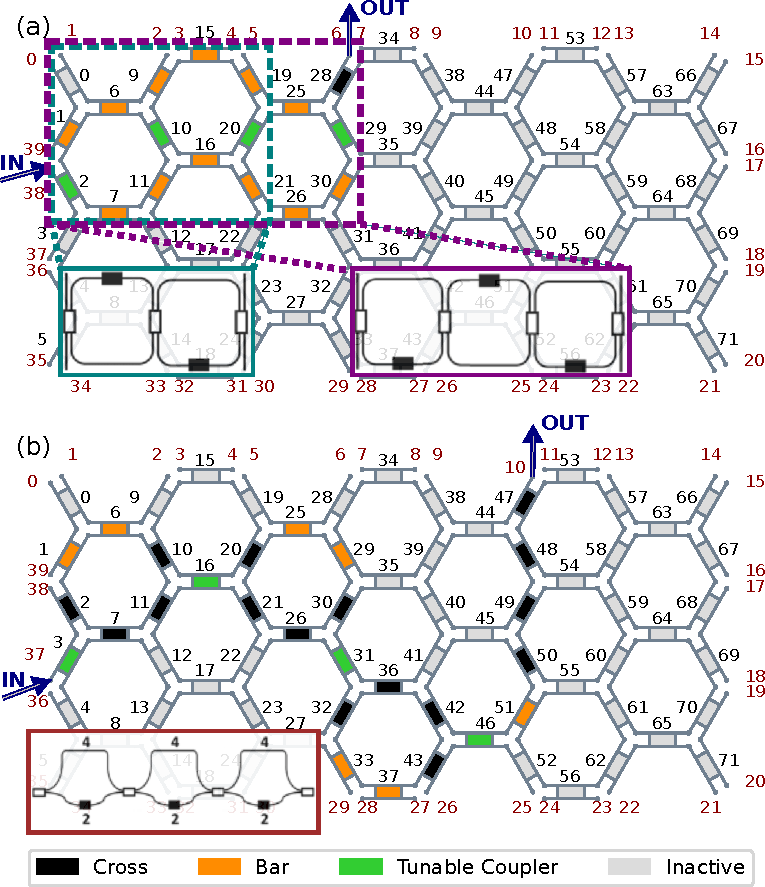
\includegraphics{figures/ch3-filters.pdf}
	\end{center}
	\caption{Optical filtering experiment.
		(a) Circuit schematic and waveguide mesh implementation of resonant (IIR) second (turquoise) and third-order (purple) CROW filters featuring coupled-ring cavities of length 6~BUL.
		(b) Circuit schematic (red box) and waveguide mesh implementation of a third-order UMZI photonic lattice filter.
	}\label{fig:ch3-filters}
\end{figure}

To demonstrate the capabilities of the programmable photonic processor, we configured the photonic waveguide mesh to implement various filter architectures and tested their performance.
The experiments demonstrated the implementation of multiple tunable filters.
The implementation of one IIR and one FIR filter is presented in Listing~\ref{lst:ch3-filters} using the developed Python API.
For the IIR case we synthesized a second (turquoise) and third-order (purple) resonant Coupled Resonant Optical Waveguide (CROW) filters, which consisted of two and three coupled-ring cavities, respectively, (see Figure~\ref{fig:ch3-filters}(a)).
These filters have two complementary outputs representing the through and drop responses of a resonant filter (refer to Section~\ref{sub:integrated_photonic_resonant_devices}).
The through response of the second-order CROW, in Fig.~\ref{fig:ch3-filters_osa}(a), exhibits a notch response with a suppression of 26 dB and a free spectral range (FSR) of 14.98 GHz.
The drop spectrum of the third-order CROW is shown in Fig.~\ref{fig:ch3-filters_osa}(b).
As expected, we observe a band-pass characteristic with an extinction ratio of 23 dB.
We notice that in this case the inclusion of another ring has increased the insertion losses of the circuit in around 10 dB.
These losses can be reduced by improving the tuning and resolution of coupling between the rings, so signal leakage can be minimized.
The right part of Figure~\ref{fig:ch3-filters_osa}(b) shows the band-pass tuning along a complete FSR where the resonance frequency could be tuned by modifying cross-phase shifters in the intracavity PUCs.
For the FIR case we implemented a third-order UMZI lattice filter (see Figure~\ref{fig:ch3-filters}(b)).
The latter exhibits a band-pass response with an extinction ratio of 21 dB and FSR of 44.95 GHz as shown in Figure~\ref{fig:ch3-filters_osa}(c) left.
This filter was fully tunable over an entire FSR interval by reconfiguring cross-phase shifters (see Fig.~\ref{fig:ch3-filters_osa}(c) right).
Both filters can be optimized by tuning the internal PUC responses and changing the zero and pole positions \cite{madsen_digital_1999}.
In \cite{perez-lopez_supplementary_2024} we provide a detailed description of the implementation and measurements of 17 additional types of filter architectures.

\begin{figure}[t!]
	\begin{center}
		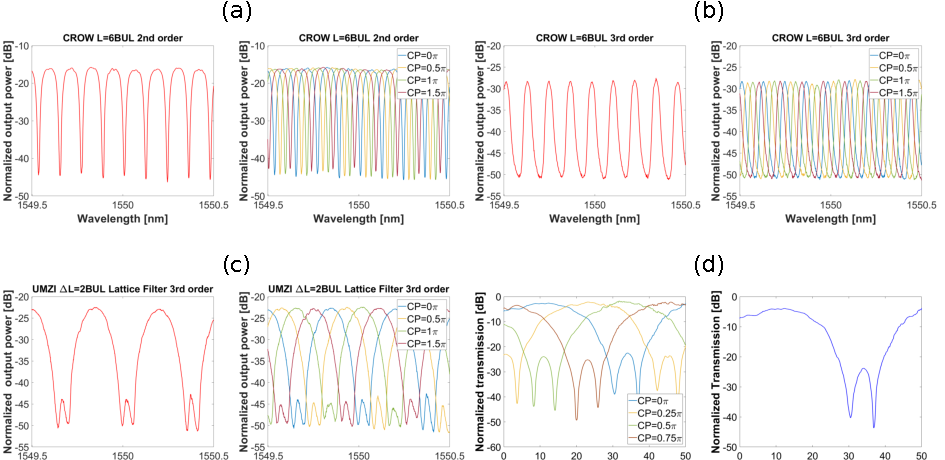
\includegraphics{figures/ch3-filters_osa.pdf}
	\end{center}
	\caption{Optical filtering demonstration.
		Third-order CROW filter featuring three coupled-ring cavities of length 6BUL: (a) Left: Spectral response for the reflection spectrum.
		Right: frequency notch tuning along a complete FSR (using an intracavity PUC as a cross-phase shifter CP).
		(b) Left: Transmission spectrum,  Right: band-pass tuning along a complete FSR (using an intracavity PUC as a cross-phase shifter CP).
		(c) Optical transfer function and the tuning of the UMZI lattice filter and (d) RF transfer function and the tuning of the MWP filter based on self-beating of the third-order UMZI photonic lattice filter. }\label{fig:ch3-filters_osa}
\end{figure}

\begin{figure}[htb]
	\begin{center}
		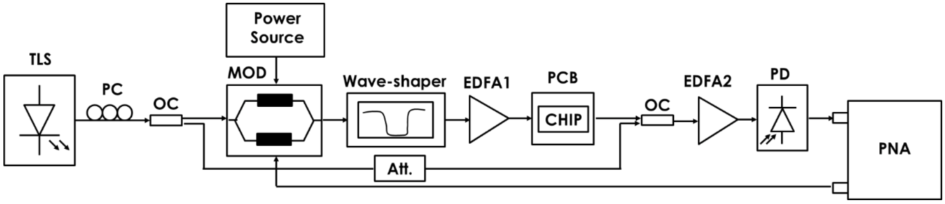
\includegraphics{figures/ch3-filters_rf_conversion.pdf}
	\end{center}
	\caption{Passive setup used to measure the radiofrequency response of the different optical filters.
	}\label{fig:ch3-filters_rf_conversion}
\end{figure}

% Tunable and reconfigurable radiofrequency filters and phase shifters
The radiofrequency response of these optical filters can be obtained from direct down-conversion of their spectrum.
For this, an input single-sideband RF signal must be employed, the optical carrier must be suppressed, re-injected and combined with the upconverted RF sideband after the latter is processed by the filter.
As depicted in Figure~\ref{fig:ch3-filters_rf_conversion}, first, an optical carrier emitted by a tunable laser source (TLS), and a vector network analyzer (PNA, Optical Network Analyzer) is used to modulate the electro-optic modulator biased at the quadrature bias point (QB).
A dual-drive modulator (MOD) was used as a modulator, in combination with a wave-shaper, implementing a stop-band filter to implement the carrier suppression and single- sideband modulation.
In addition, we used two optical couplers (OC) at the input (50/50) and output (50/50) to implement the self-beating technique.
The SSB modulated signal is amplified by an erbium-doped fiber amplifier (EDFA) from and introduced to the optical integrated filter synthesized in the photonic mesh.
Once the signal is outside the chip, it is amplified again with another EDFA for compensating the losses suffered in the integrated chip, and photo detected and sent to the microwave network analyzer (PNA) to measure the transmission response.

% We assembled a testing and measurement setup as described in Supplementary Note 5 to measure the implementation of MWP filters based on different photonic filters.
Figure~\ref{fig:ch3-filters_osa}(d) shows the transfer function and the tuning of an MWP filter based on the third-order UMZI photonic lattice filter described previously.
Note that the filter displays an RF power extinction ratio of 40 dB and features a radiofrequency FSR of 44 GHz (matching its photonic counterpart).
The interested reader is directed to Supplementary Note 5 of \cite{perez-lopez_supplementary_2024} for the implementation details of other microwave photonic filters.
It is important to highlight here that, when compared to application-specific photonic circuits, the programmable processor suffers from extra excess losses due to the waveguide lattice mesh, reducing the total RF gain of the filter.
To overcome this limitation, the integration of optical amplifiers in the system can be considered as discussed in Section~\ref{sub:amplification}.

% section Filters (end)

\section{Reconfigurable delay lines}\label{sec:reconfigurable_delay_lines} % (fold)

True time optical delay lines (TTODLs) are important because they enable precise, dynamically adjustable delays in photonic circuits, which are essential for advanced microwave photonics applications \cite{lenz_optical_2001,xiang_low-loss_2018,zhu_silicon_2020}.
By providing a means to finely control signal timing and phase, TTODLs are instrumental in beamforming networks where accurate synchronization of signals across an antenna array is vital for steering beams without distortion or squint.
% The latter capability is particularly important for wideband applications in next-generation wireless communications, radar, and optical filtering.
TTODLs solve the beam squint problem by providing frequency-independent phase shifting, which ensures that signals at different frequencies experience the same time delay.
In traditional phased array systems that use phase shifters, the delay introduced is proportional to the signal's wavelength.
This is solved by introducing actual path differences between the signals so that a constant time delay is introduced instead of a phase shift.
Moreover, integrating TTODLs into waveguide mesh architectures offers significant advantages over traditional static delay lines.
As proposed by \cite{perez-lopez_programmable_2018}, it allows for a compact, reconfigurable, and programmable platform that can adapt to varying system requirements in real time.

\begin{figure}[t!]
	\begin{center}
		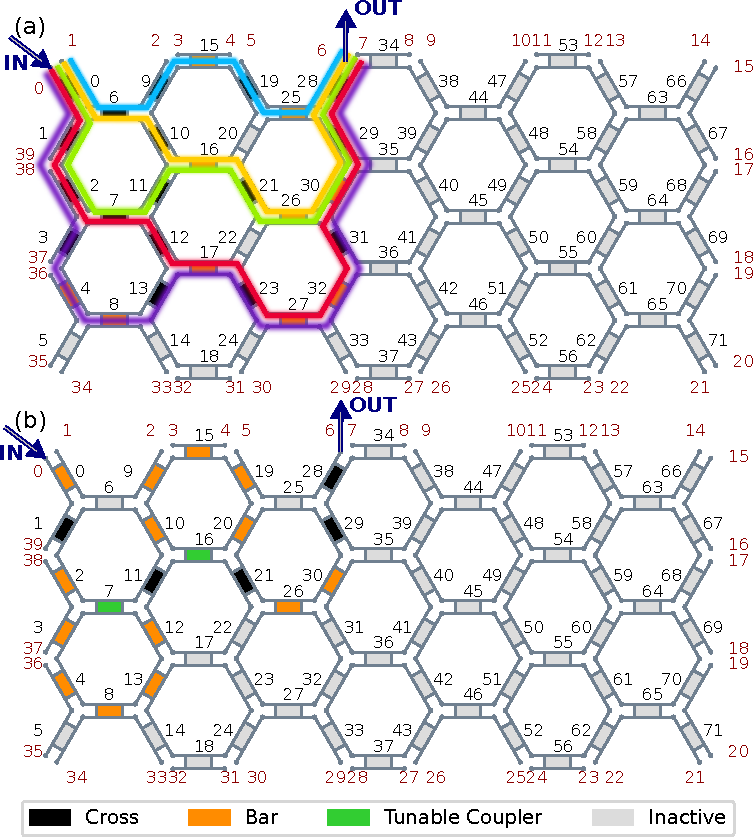
\includegraphics{figures/ch3-delay_circuits.pdf}
	\end{center}
	\caption{Optical delay lines experiment.
		(a) Schematic of discrete delay lines on the hexagonal mesh using port 0 and 6 as input and output, respectively.
		Longer paths are used to introduced higher delays.
		(b) Schematic of a SCISSOR filter used to generate a continuous delay response between discrete steps.
	}\label{fig:ch3-delay_circuits}
\end{figure}

In this work we present the implementation of discrete and continuous delay lines on the iPronics first-generation Smartlight platform.
The code implementation of both can be found in Listing~\ref{lst:ch3-delay_circuits} where both discrete and continuous circuits are detailed.
The first are represented by the overlap of interconnect paths of different lengths with a minimum \(\Delta L = 2\cdot BUL\) (or \(\Delta \tau = 2\cdot \tau_{BUL}\)) where \(BUL = 811.41 \mu m\) (or \(\tau_{BUL} = 11.25 ps\)).
The \(2\cdot \) constrain emerges from the hexagonal architecture.
The time delay performance of each path was measured with the processor fed with an input pulsed signal from a LUNA optical vector analyzer (OVA).
The different paths configurations were programmed on the processor and their time responses measured with the OVA which provided the amplitude and delay characteristics of each input/output port pair.
As observed in Figure~\ref{fig:ch3-delay_luna}(a), the peak response of the different paths are consistently spaced by \(22.5\,ps\) as expected, with their responses only being different by a decreasing peak amplitude.
The latter occurs due to the increasing insertion losses of adding 2 more PUCs to each longer path.
Recall that the reported losses of this platform are \(IL_{PUC} \approx 0.46\) dB.
\\ % New linte to avoid splitting listing

\begin{lstlisting}[caption={Configuration of discrete and continuous delay lines using the first-generation Smartlight API}, label=lst:ch3-delay_circuits]
	# Discrete delays
	delay_1 = [
		(0, "x"), (6, "="), (9, "x"), (15, "="), (19, "x"), (25, "="),
		(28, "="),
	]
	delay_2 = [
		(0, "x"), (6, "x"), (10, "x"), (16, "x"), (21, "x"), (26, "="),
		(30, "="), (29, "x"), (28, "x"),
	]
	# Continuous delay
	scissor = [
		(0, "="), (1, "x"), (2, "="), (7, k1), (12, "="), (13, "="),
		(8, "="), (4, "="), (3, "="), (11, "x"), (16, k2), (10, "="),
		(9, "="), (15, "="), (19, "="), (20, "="), (21, "x"), (26, "="),
		(30, "="), (29, "x"), (28, "x"),
	] % k1=k2=0.05
	puc_info = scissor # delay_1+delay_2
	smart.manual_circuit_configuration(puc_info)
	set_coupling_factor_phase([(8, ["=", cp]), (15, ["=", -1*cp])])
\end{lstlisting}

\begin{figure}[h]
	\begin{center}
		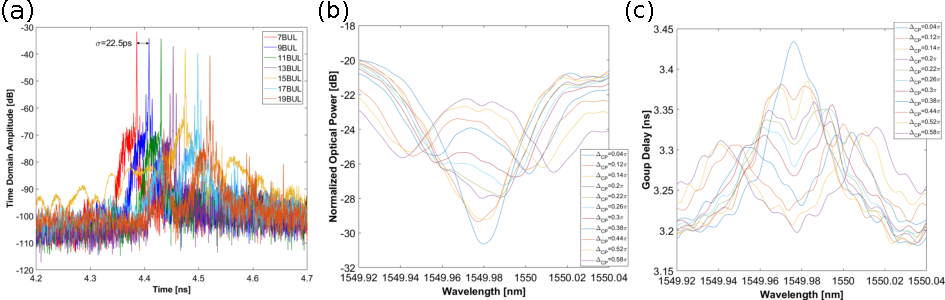
\includegraphics{figures/ch3-delay_luna.pdf}
	\end{center}
	\caption{Reconfigurable delay line demonstration.
		(a) Discrete time delay steps observed through an optical vector analyzer (OVA) with steps of 22.5~ps observed.
		(b) Transmission response of the SCISSOR circuit when applying different cross-phases to detune the resonance wavelengths of its inner rings in order to achieve different group delay responses.
		(c) Continuous time delay yielded by detuning the rings of a SCISSOR circuit through different cross-phases.
		Different values of cross-phases lead to different values of group delay at the transmission port.
		The continuous delay is observed to cover a span of 0.24~ns.
	}\label{fig:ch3-delay_luna}
\end{figure}

The continuous delay demonstration is performed by synthesizing the SCISSOR circuit in Listing~\ref{lst:ch3-delay_circuits}.
To measure the time response we employed the OVA connected to both the input and output of the SCISSOR structure.
The first step was to tune both rings so that their resonances match.
To achieve this, we use the \lstinline|set_coupling_factor_phase()| instruction on PUCs 8 and 15 to perform the fine-tuning until reaching the resonant point (See Fig.~\ref{fig:ch3-delay_luna}(b) for \(\Delta_{CP}=0.04 \pi \)).
From here we performed a detuning of the rings by adding an asymmetric offset to the cross-phases of PUCs 8 and 15.
When this detuning happens the amplitude response of the filter changes and, due to the dispersive nature of this structure, its group delay also changes.
This effectively introduces a continuous delay line which can be controlled by the cross-phase tuning.
In Figure~\ref{fig:ch3-delay_luna}(c), we observe that the maximum continuous delay span that can be obtained with this method is of 0.24~ns, which is more than enough to fill the discrete steps presented in the discrete example.
A combination of both discrete and continuous delay lines could be implemented on a larger mesh with more recirculating cells where each arm can be loaded by a SCISSOR structure.
This would enable smooth beam steering applications where the coarse delay is added with interconnect paths and the fine delay is inserted by the ring detuning.
Certainly, such a large scale solution will require that PUCs are small so that insertion losses, time step \(\Delta_{BUL}\) and area can be minimized \cite{perez-lopez_integrated_2019}.
We also denote that the loss penalty for introducing the continuous delay can reach \(\approx 9\) dB for the entire 0.24~ns span.
However, it's important to consider that in order to cover the full range between two discrete delay steps (22.5~ps), the expected loss is \(\approx 1\) dB, which is comparable to the discrete step penalty.

% section Continuous delay lines (end)

\section{Topological photonic arrays}\label{sec:topological_photonic_arrays} % (fold)

\begin{figure}[b!]
	\begin{center}
		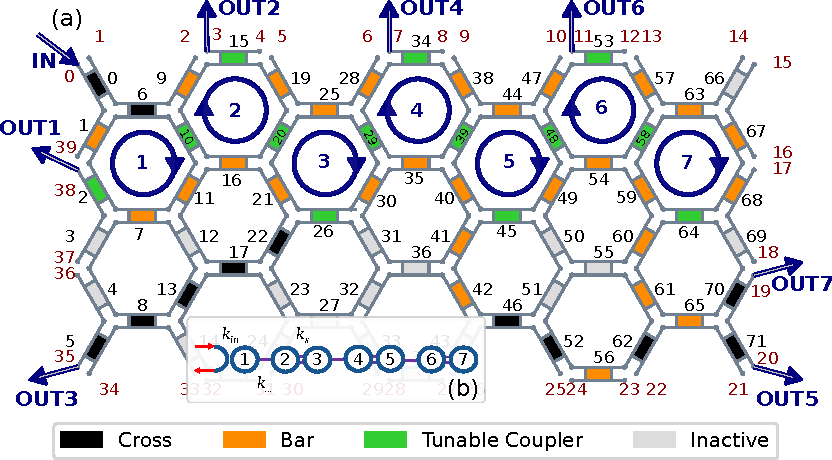
\includegraphics{figures/ch3-topological-ssh.pdf}
	\end{center}
	\caption{(a) Implementation of the Su-Schrieffer-Heeger (SSH) model circuit using seven ring resonators and optical paths to tap out signal power. (b) Schematic of the implemented 1D SSH model.}\label{fig:ch3-topological_ssh}
\end{figure}

% In this section we explore the use of programmable photonic circuits to implement topological Hamiltonians within a single reconfigurable platform \cite{on_programmable_2024}.
Topological photonics can trace its roots to the discovery of topological insulators in condensed matter physics \cite{klitzing_new_1980,thouless_quantized_1982}, where bulk materials that are naturally insulating can conduct electricity under certain conditions.
These concepts have been replicated in the photonics world \cite{ozawa_topological_2019,price_roadmap_2022}, where topology refers to a quantized property that describes the global behavior of the wavefunctions in a dispersion band.
A key feature of topological photonics is the existence of modes that live on the edge of photonic materials with non-trivial topologies and that show resilience to certain types of disorder.
While topological photonics has led to significant advancements in areas such as lasing, sensing, and quantum technologies \cite{shalaev_robust_2019,bahari_nonreciprocal_2017,ezawa_higher-order_2018,blanco-redondo_topological_2018}, existing experimental implementations typically support only fixed topological models with limited or no reconfigurability.
Here, we document how this limitation can be overcome by using the first-generation Smartlight programmable silicon photonic mesh to allow real-time control of key parameters such as hopping strengths, phase shifts, and on-site potentials.
This reconfigurable approach positions programmable photonics as a universal testbed for exploring topological physics and novel photonic devices, accelerating research in non-Hermitian photonics, quantum optics, and programmable photonic computing.
In \cite{on_programmable_2024}, we demonstrate the versatility of this approach by experimentally implementing the 1D Su-Schrieffer-Heeger (SSH) model, which supports robust edge states, and simulating the 2D breathing Kagome lattice, which hosts higher-order topological corner states.
In this section we present the circuit and the experimental results obtained from the former model.

The Su-Schrieffer-Heeger is the simplest topological model \cite{su_solitons_1979}.
It's a dimmer chain which is composed by an alternate pattern of weak and strong coupling between sites.
Here, we implement the SSH model in the hexagonal mesh by configuring it as a bipartite lattice of seven ring resonators connected with one another as shown in Fig.~\ref{fig:ch3-topological_ssh}(b).
The equivalent synthesized circuit on the programmable mesh is marked by blue circumferences in Fig.~\ref{fig:ch3-topological_ssh}(a).
The Python code needed to implement this circuit on the programmable core is presented in Listing~\ref{lst:ch3-topological_ssh}.

The Hamiltonian describing this system of rings is given by

\begin{equation}
	H = \left[ k_w \sum_{n \in \{1,3,5\}} a_n^\dagger a_{n+1} + k_s \sum_{n \in \{2,4,6\}} a_n^\dagger a_{n+1} \right] + H.c.
	\label{eq:ch3-topological_ssh}
\end{equation}

where $k_w$ and $k_s$ are the strong and weak coupling strengths between sites, and $a_n^\dagger$ and $a_n$ are the creation and annihilation operators on site $n$.
Note that these variables are directly translated to the coupling factor settings in Listing~\ref{lst:ch3-topological_ssh}.
Also notice that optical paths have been configured on the mesh to tap some power from the rings using the on-chip photodetectors.
Specifically, 1\% of the power is coupled out using PUCs as couplers.

\begin{lstlisting}[caption={Implementation of the Su-Schrieffer-Heeger (SSH) model using the first-generation Smartlight API}, label=lst:ch3-topological_ssh]
rings = [ 
    (0, "x"), (1, "="), (2, 0.01), (6, "x"), (7, "="), (9, "="),
    (10, k_w), (11, "="), (15, 0.01), (16, "="), (19, "="),
    (20, k_s), (21, "="), (25, "="), (26, 0.01), (28, "="),
    (29, k_w), (30, "="), (34, 0.01), (35, "="), (38, "="),
    (39, k_s), (40, "="), (44, "="), (45, 0.01), (47, "="),
    (48, k_w), (49, "="), (53, 0.5), (54, "="), (57, "="),
    (58, k_s), (59, "="), (63, "="), (64, 0.01), (67, "="),
    (68, "="),
]
pd_paths = [
    (5, "x"), (8, "x"), (13, "x"), (17, "x"), (22, "x"), (41, "="),
    (42, "="), (46, "x"), (52, "x"), (56, "="), (62, "x"),
    (60, "="), (61, "="), (65, "="), (70, "x"), (71, "x"),
]
su_schrieffer_heeger = rings + pd_paths
smart.manual_circuit_configuration(su_schrieffer_heeger)
\end{lstlisting}

Figure~\ref{fig:ch3-topological-power_meter} shows that by configuring the mesh into a dimerized lattice and alternating the coupling strengths between sites (using the coupler PUCs to set $k_w$ and $k_s$), we enable the formation of topologically protected edge states.
The calculated eigenvalues of this lattice, represented here by the resonant frequencies of the supermodes, are shown in Figure~\ref{fig:ch3-topological-power_meter}(a) for four different combinations of $k_w$ and $k_s$, which is referred as the dimerization pattern from now on.
The experimental measurements in Figure~\ref{fig:ch3-topological-power_meter}(b) confirms that in the topological phase, light remains strongly localized at the system’s boundary, while virtually zero power is measured in the even rings.
The robustness of the edge state is further tested by introducing disorder in the coupling strengths, showing that the topological mode persists even under perturbations.
Figure~\ref{fig:ch3-topological-power_meter}(c-d) shows the power sum in all the even and odd rings when the input laser is swept $\pm$ 6 GHz from its central frequency $f_0=193 THz$.
Here, we observe that stronger dimerization patterns lead to larger band gaps and more pronounced edge localization.
This is because the only supermode supported around $f_0$ is the topological edge mode, which is fully localized in the odd rings.
The residual amount of power observed in the even rings at f0 is due to the non-perfect overlap of the input light with the modal profile of the edge mode.
These results highlight the ability of the programmable platform to precisely tune topological properties.

\begin{figure}
	\begin{center}
		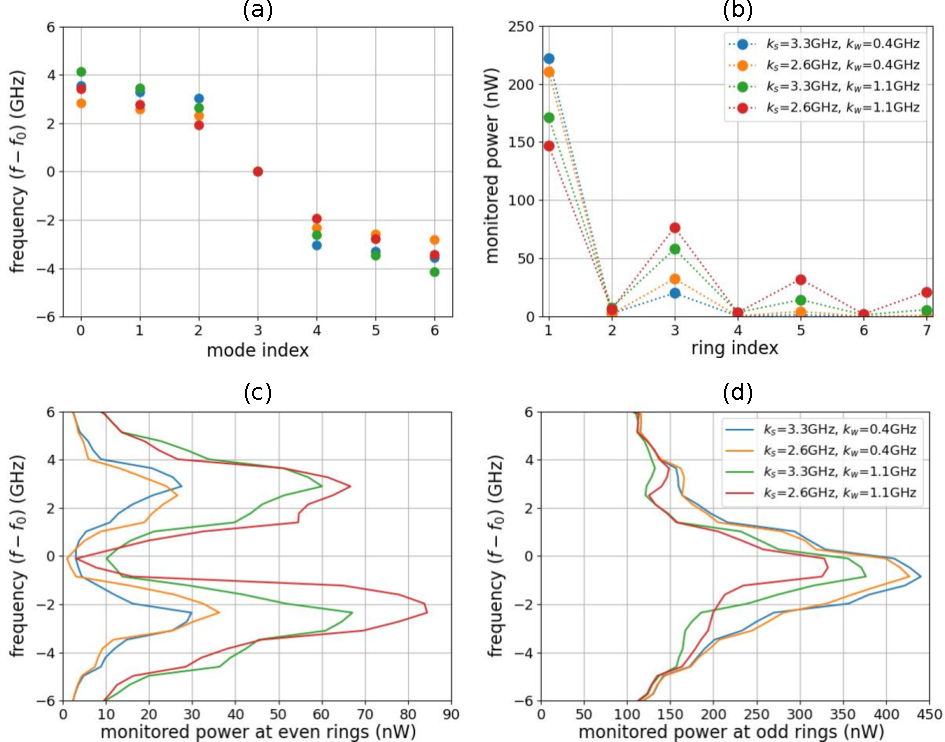
\includegraphics{figures/ch3-topological-power_meter.pdf}
	\end{center}
	\caption{Characterization of the eigenvalues and the topological edge mode in the SSH model. (a) Calculated eigenvalues of the Hamiltonian matrices. (b) Monitored powers (tapped ≈ 1\% of the power in
		each ring) at the coupled ring resonators from the programmable mesh hardware. (c) Total monitored power (tapped ≈ 1\%) spectrum of the even rings of 1D SSH model. (d) Total monitored power spectrum
		of the odd rings of 1D SSH model.}\label{fig:ch3-topological-power_meter}
\end{figure}

% section Topological photonic arrays (end)

\section{Optical Max Pooling}\label{sec:optical_max_pooling} % (fold)

\begin{figure}[b!]
	\begin{center}
		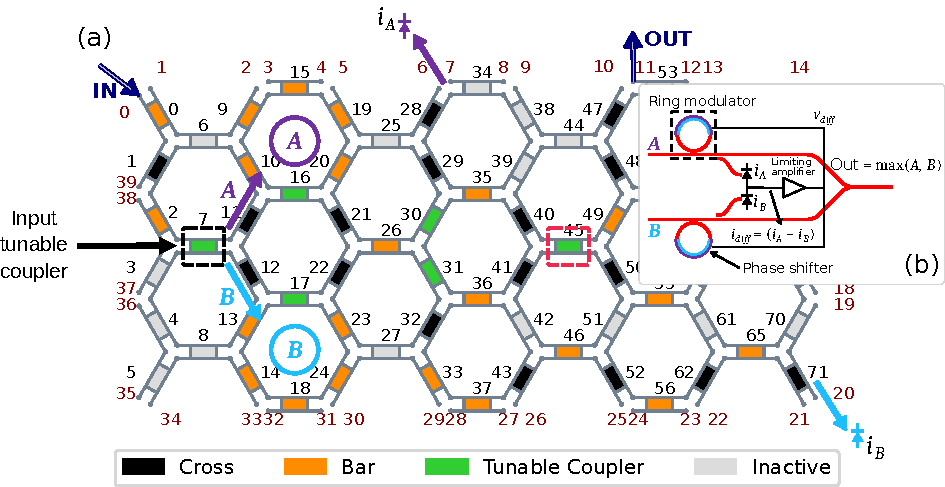
\includegraphics{figures/ch3-maxpool-circuit.pdf}
	\end{center}
	\caption{(a) Implementation of the proposed max pooling circuit on a programmable photonic platform.  (b) Proposed max pooling architecture using integrated ring modulators}\label{fig:ch3-maxpool-circuit}
\end{figure}

PICs have attracted attention as a solution to address the growing computational demands of deep neural networks (DNNs) and the limitations of traditional digital hardware, such as GPUs, as a platform to reduce power consumption and improve computational speed.
Experimental demonstrations of the building blocks of neural networks such as multiply and accumulate (MAC) \cite{feldmann_parallel_2021,tait_neuromorphic_2017,ashtiani_-chip_2022} and all-optical/optoelectronic activation functions \cite{jha_reconfigurable_2020} have been published as standalone and system solutions.
The former MAC case and its implementations in a programmable photonic platform will be discussed in detail in Chapter~\ref{chap:universal_unitary_operators}.
Here we cover the optoelectronic implementation of a popular activation function: Pooling.
Pooling layers are used to downsample an input tensor by calculating the average (average-pooling) or maximum (max pooling) of its components.
Max pooling is commonly used to reduce computation load, improve feature extraction, and enhance invariance to input transformations \cite{murray_generalized_2014,zhang_winner-take-all_2020}.
While average pooling can be easily implemented using linear optical components, max pooling requires nonlinear processing making it difficult to implement directly using passive integrated components.
In this section we address this challenge by using optical ring modulators whose resonance conditions dynamically shift based on input power differences, effectively allowing the system to select the maximum input value \cite{ashtiani_photonic_2023}.

Figure~\ref{fig:ch3-maxpool-circuit} shows the proposed circuit synthesized on the programmable core alongside its target schematic.
Note that the circuit relies on an optoelectronic feedback loop to drive the ring modulators so that their notch responses are used to either suppress (discard) or pass (pool) one of the two input signals $(A,B)$.
Initially the rings' resonances are tuned and positioned symmetrically around \(\lambda_0\) so that the two signals go through.
A small fraction of the optical power from each ring is tapped using tunable couplers and sent to the on-chip photodetectors (PDs).
The PDs measure the power of each signal and are arranged to yield the proportional electrical current difference \(i_{diff} = i_A - i_B\).
This difference current is then amplified using a limiting amplifier, which ensures that the output voltage is constrained to two discrete levels, \(V_A\) and \(V_B\) which bring each ring resonance to \(\lambda_0\) and induce strong attenuation.
If \(A>B\) (\(B>A\)), the system shifts the resonance of ring \(B\)($A$) to align with \(λ_0\), heavily attenuating \(B\)($A$) while allowing \(A\)($B$) to pass.

\begin{equation}
	\text{Output} = \max(A, B)
	\label{eq:ch3-maxpool}
\end{equation}

The closed-loop feedback system ensures that even small differences between \(A\) and \(B\) are detected, making the system highly sensitive.
Since one ring is always locked to the operation wavelength \(λ_0\), the architecture remains stable and resistant to external perturbations or drift.

\begin{lstlisting}[caption={Impementation of an optical max pooling architecture using the first-generation Smartlight API.}, label=lst:ch3-maxpool-circuit]
maxpool_rings = [
    (0, "="), (1, "x"), (2, "="), (7, k_in), (9, "="), (10, "="),
    (11, "x"), (12, "x"), (13, "="), (14, "="), (15, "="),
    (16, 0.5), (17, 0.5), (18, "="), (19, "="), (20, "="),
    (21, "x"), (22, "x"), (23, "="), (24, "="), (26, "="),
]
maxpool_pds = [
    (28, "x"), (29, "x"), (30, 0.01), (31, 0.01), (32, "x"), (33, "="),
    (35, "="), (36, "="), (37, "="), (40, "x"), (41, "x"), (43, "x"),
    (45, 0.5), (46, "="), (47, "x"), (48, "x"), (49, "="), (50, "x"),
    (52, "x"), (55, "="), (56, "="), (60, "x"), (62, "x"), (64, "x"),
    (65, "="), (68, "x"), (71, "x"),
]
maxpool = maxpool_rings + maxpool_pds
smart.manual_circuit_configuration(maxpool)
\end{lstlisting}

\begin{figure}[b!]
	\begin{center}
		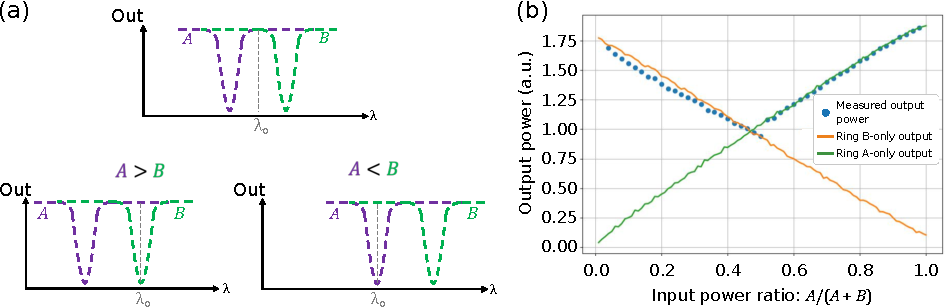
\includegraphics{figures/ch3-maxpool-power_meter.pdf}
	\end{center}
	\caption{
		(a) Expected the transfer characteristics of the proposed max-pooling operator for different input scenarios.
		(b) Output power of the photonic max-pooling circuit as a function of the input power ratio.}\label{fig:ch3-maxpool-power_meter}
\end{figure}

The implementation of this circuit is presented in Listing~\ref{lst:ch3-maxpool-circuit}.
Note that in this experiment a single input is used to simplify the setup.
The two inputs are generated by tuning \(k_{in}\) to split the input laser into two signals of different powers to feed the max pooling circuit.
The power tapped is then routed to the peripheral PDs and the amplification operation is performed digitally by the logic unit (LU).
The driving signals for the ring resonators were applied on the phase actuators to close the loop.
Figure~\ref{fig:ch3-maxpool-power_meter}(a) exemplifies the functioning mechanism of the proposed solution while (b) shows the measured results demonstrating the pooling operation.
The latter shows that depending on \(k_{in}=A/(A+B)\) one output or the other is selected by the circuit, effectively demonstrating the nonlinear max pooling operation.
It can be seen that at any input power ratio, the output selects the larger input.
Note that by using fast modulators (e.g., PN-junction modulator) and wideband limiting amplifiers, bandwidths of tens of GHz (i.e., picosecond response time) can be achieved.

% section Optical Max Pooling (end)

% chapter Applications using FPPGAs (end)

% Author: David Sanchez-Jacome

\chapter{Universal Unitary Operators}\label{chap:universal_unitary_operators} % (fold)

Linear optical operations lie at the heart of several optical systems.
For example, optical hybrids are key components in Telecom coherent receivers \cite{faralli_compact_2015}, discrete Fourier transform (DFT) operators enable high-fidelity FMCW Lidar \cite{kim_fmcw_2020}, quantum information processing is performed using linear quantum logic gates \cite{arrazola_quantum_2021,harris_large-scale_2016}, signal processing in radar \cite{sanchez-jacome_coherent_2021} and multicore fiber systems \cite{sakamoto_strongly-coupled_2017} relies on the multiple-input and multiple-output (MIMO) technique to unscramble the signals and recover the information (i.e., a unitary matrix operation); among many other use cases \cite{carolan_universal_2015}.
Such operations are usually implemented by complex custom hardware systems that can't be reused for other applications.
Nevertheless, specific optical system architectures that can implement all these unitary operations on the same hardware are known to exist in bulk and integrated optics \cite{clements_optimal_2016}.
The feasibility studies to implement such unitary operations on programmable integrated platforms have gained significant attention and resources in the last decade.
It's expected that the solid-state nature of these devices will enhance the cost-efficiency, mass-manufacturability, and reusability of integrated unitary operators within several application fields.

In parallel to the development of universal unitary operators' theory, recent years have also seen the rise of software-defined integrated photonic solutions with applications in microwave photonic systems, data center interconnects, reconfigurable beam-splitting and optical filtering/processing \cite{perez-lopez_general-purpose_2024}.
Such solutions, based on a hexagonal mesh of recirculating cells, are composed of programmable unit cells (PUCs), i.e., 2x2 Mach-Zehnder interferometers (MZI), that can be reconfigured into different states by tuning their arm-loaded phase shifters.
By adequately setting these states on concatenated PUCs one can synthesize several kinds of photonic circuits on the same hardware platform.

Among the circuits these hexagonal meshes can implement we find the aforementioned architectures that can perform all unitary transformations \cite{carolan_universal_2015, clements_optimal_2016}.
The procedure to map these custom architectures to a recirculating hexagonal mesh was reported in \cite{perez_silicon_2017}.
To the best of our knowledge, this is the only experimental demonstration of unitary operators on a hexagonal mesh.
However, when this work was done, the mesh size was composed of seven recirculating cells only, thus limiting the maximum size of unitary operators to 4x4.
Additionally, at the time, the phase values had to be calculated, set, and fine-tuned manually to produce the desired objective matrix on the mesh due to the lack of an autoconfiguration layer driving the silicon photonics chip.
In the last five years, this field has matured significantly to the point where up to 72 unit cells in the core are currently commercially available \cite{perez-lopez_general-purpose_2024}.
The latter platforms can allocate larger unitary operators and concatenate them with other circuits in a place and route manner on the same device, thus enabling developers to explore a previously unavailable space of applications.

This chapter addresses the scalability and autoconfiguration issues observed in previously reported linear operators on hexagonal meshes.
We start by presenting the novel mathematical work developed during this dissertation to translate a Clements-based MZI phase configuration to a hexagonal one.
We continue by covering the calibration routine needed to synthesize such circuit on the hexagonal core.
Then, we proceed by introducing the instruction set developed to automatically synthesize unitary operators on the iPronics first-generation Smartlight hexagonal chip architecture.
The chapter finalizes with the experimental demonstration of applications for the optical communications field.
First, we present two operators of sizes 3 and 4 acting as 120$^o$, and 90$^o$ hybrids, respectively, typically employed in coherent transceivers.
Finally, a 6-by-6 operator is demonstrated, implementing multicast switching for wavelength division multiplexing (WDM) reconfigurable optical add-drop multiplexers (ROADMs).

\section{Feedforward to Hexagonal translation}\label{sec:feedforward_to_hexagonal_translation} % (fold)

The mathematical decomposition required to implement any unitary operator using the rectangular so-called Clements mesh has been widely documented \cite{clements_optimal_2016, capmany_programmable_2020}.
The procedure is based on splitting the target matrix in 2-by-2 elements, nulling the non-diagonal elements so that the transformation can be represented as the concatenated response of several PUCs as seen in Section~\ref{sub:the_mach-zehnder-interferometer}.
When arranged carefully these 2-by-2 gates can conform rectangular \cite{clements_optimal_2016}, triangular \cite{reck_experimental_1994}, diamond \cite{shokraneh_diamond_2020} among other documented architectures \cite{miller_self-configuring_2013}.
For example, find the actual implementation of a Clements mesh array in Figure~\ref{fig:ch4-mapping_feedforward}, which is the one we will work with in the current chapter and refer from now on as the feedforward architecture.
We denote that the hexagonal core can similarly implement the other architectures aforementioned, but that study lies beyond the scope of this text.
A unitary operator can then be decomposed into the phases that will be driven on the phase shifters so that the transfer function of this system will be equal to unitary operator multiplied by the input vector \cite{taballione_universal_2021, arrazola_quantum_2021, ruocco_demonstration_2016}.
For details about the actual mathematical decomposition procedure the interested reader may refer to \cite{clements_optimal_2016, capmany_programmable_2020}.
What is less documented is that such transformations can also be implemented using general purpose, recirculating meshes such as the one covered in Chapter~\ref{chap:fundamentals} and presented in Figure~\ref{fig:ch4-mapping_feedforward}.
For this to be possible, another transformation must be performed so that the feedforward architecture can be mapped to the multipurpose hexagonal core.
An initial attempt to cover this mapping was presented by \cite{perez_silicon_2017}, however this implementation still relied on manual fine-tuning after the phase driving to achieve the desired transformation.

\begin{figure}[h!]
	\begin{center}
		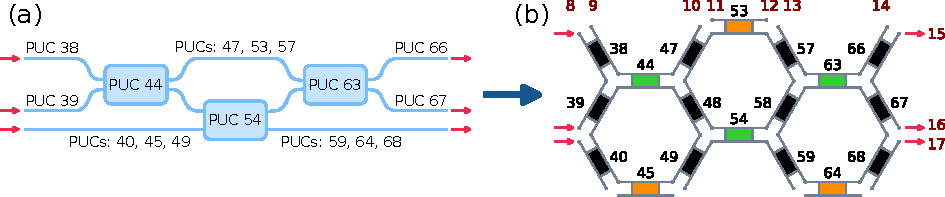
\includegraphics{figures/ch4-mapping_feedforward.pdf}
	\end{center}
	\caption{Mapping between the Clements \cite{clements_optimal_2016} feedforward operator circuit (a) of dimension 3 and its implementation in the hexagonal mesh (b)}\label{fig:ch4-mapping_feedforward}
\end{figure}

The iPronics v1 and v2 meshes can allocate a unitary matrix size of up to 6-by-6.
Obviously smaller unitary operators can be implemented using smaller subsections of the core and larger sizes will have to be split in tiles as needed to fit in this core.
However, the equations derived to map the phases used by a feedforward multi-port interferometer (e.g., Clements or Reck) into the phases to be programmed on a hexagonal waveguide mesh arrangement are agnostic to the matrix size.
Here we summarize the phase equivalence equations obtained for the three different scenarios that can be encountered when implementing such circuits.
Such translation defines a series of phase values that can be used to drive the MZI actuators and then implement the linear matrix multiplication in the hexagonal integrated waveguide array.

\subsection{The feedforward PUC}\label{sub:the_feedforward_puc} % (fold)

The feedforward PUC consists of a single-loaded MZI preceded by a phase shift at one input port.
We can map such structure to our hexagonal mesh by translating the MZI with the phase shifter using a trilattice formed by three PUCs.
Schematically this mapping could be visualized as in Figure~\ref{fig:ch4-mapping_trilattice}.
\begin{enumerate}
	\item Blue PUC: External phase shifter
	\item Orange PUC: Photonic wire
	\item Green PUC: Balanced MZI
\end{enumerate}

\begin{figure}[h!]
	\begin{center}
		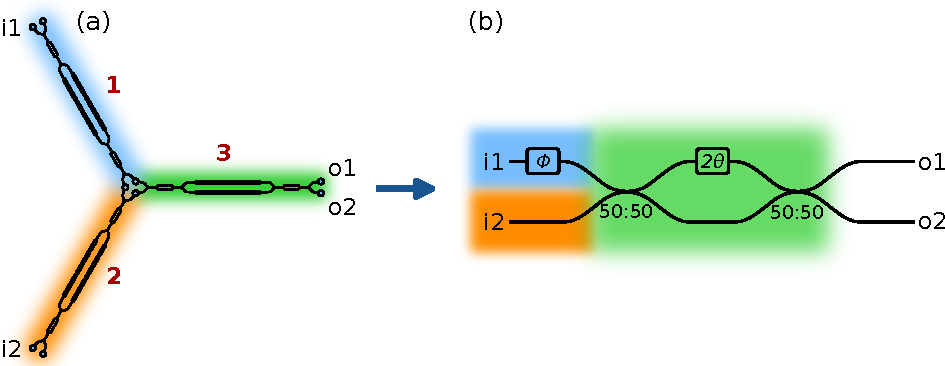
\includegraphics{figures/ch4-mapping_trilattice.pdf}
	\end{center}
	\caption{Mapping of the MZI and the phase shifter in a feedforward mesh (a) using the hexagonal
		architecture (b)}\label{fig:ch4-mapping_trilattice}
\end{figure}

In order for these two structures to have the same behavior, we have to equalize their corresponding transfer function responses so that all the elements match.
On one hand, the matrix representing the FF-PUC is given by \eqref{eq:t_ff}

\begin{equation}
	\label{eq:t_ff}
	T_{FF} = je^{j\frac{\theta}{2}}
	\begin{bmatrix}
		e^{j\phi} sin(\frac{\theta}{2}) & cos(\frac{\theta}{2})  \\
		e^{j\phi} cos(\frac{\theta}{2}) & -sin(\frac{\theta}{2})
	\end{bmatrix}
\end{equation}
where $\phi$ is the external actuator phase and $\theta$ is the PUC's phase shifter value.

On the other hand, the matrix representing the dual-driven PUC present in the hexagonal mesh is given by Equation~\eqref{eq:t_hex}

\begin{equation}
	\label{eq:t_hex}
	T_{H} = je^{j\Delta}
	\begin{bmatrix}
		sin(\theta) & cos(\theta)  \\
		cos(\theta) & -sin(\theta)
	\end{bmatrix}
\end{equation}
where $\Delta = (\phi_{up} + \phi_{lo})/2$ and $\theta = (\phi_{up} - \phi_{lo})/2$.

For the translation we need to make sure that the response of the PUC in Figure~\ref{fig:ch4-mapping_trilattice}(b) is equal to the composite version in (a).
If we address the elements in the matrices in \eqref{eq:t_ff}, \eqref{eq:t_hex} using the $i,j$ subscripts, where
$i$ and $j$ represent the row and column indices of the matrix we can relate the elements in Fig.~\ref{fig:ch4-mapping_trilattice} (a) and (b) by equating

\begin{equation}
	\label{eq:t_ff_hex0}
	T_{10} = T^{1}_{01}T^{3}_{10} \end{equation}

Where the left-hand side corresponds to the feedforward transfer function element and the right-hand side to the hexagonal one.
The upper-scripts refer to the PUC index in Fig.~\ref{fig:ch4-mapping_trilattice}.
Replacing in \eqref{eq:t_ff_hex0} with the corresponding matrix elements for both cases we obtain that

\begin{equation}
	\label{eq:t_ff_hex1}
	je^{j\frac{\theta_{FF}}{2}}cos(\frac{\theta_{FF}}{2})e^{j\phi_{FF}} = (je^{j\Delta^{(1)}_{H}}cos(\theta^{(1)}_{H}))(je^{j\Delta^{(3)}_{H}}cos(\theta^{(3)}_{H}))
\end{equation}

Where the left-hand side corresponds to the feedforward transfer function element and the right-hand side to the hexagonal one.
Solving for $\phi^{(1)}_{up}$, $\phi^{(1)}_{lo}$, $\phi^{(3)}_{up}$ and $\phi^{(3)}_{lo}$ we get

\begin{equation}
	\label{eq:map_ff_hex_1}
	\phi^{(1)}_{up} = \phi^{(1)}_{lo} = \phi_{FF} - \frac{\pi}{2}
\end{equation}

\begin{equation}
	\label{eq:map_ff_hex_2}
	\phi^{(3)}_{up} = \theta_{FF},\; \phi^{(3)}_{lo} = 0
\end{equation}

The equations for PUC\(_2\) in Fig.~\ref{fig:ch4-mapping_trilattice}(a) are obtained by equating

\begin{equation}
	\label{eq:t_ff_hex2}
	T_{11} = T^{2}_{10}T^{3}_{11} \end{equation}

Where the left-hand side corresponds to the feedforward transfer function element and the right-hand side to the hexagonal one.
Replacing in \eqref{eq:t_ff_hex2} with the corresponding matrix elements for both cases we obtain that

\begin{equation}
	\label{eq:t_ff_hex3}
	-je^{j\frac{\theta_{FF}}{2}}sin(\frac{\theta_{FF}}{2}) = (je^{j\Delta^{(2)}_{H}}cos(\theta^{(2)}_{H}))(-je^{j\Delta^{(3)}_{H}}sin(\theta^{(3)}_{H}))
\end{equation}

Solving for $\phi^{(2)}_{up}$, $\phi^{(2)}_{lo}$ one obtains

\begin{equation}
	\label{eq:map_ff_hex_3}
	\phi^{(2)}_{up} = \phi^{(2)}_{lo} = - \frac{\pi}{2}
\end{equation}

Equations~\eqref{eq:map_ff_hex_1}, \eqref{eq:map_ff_hex_2} and \eqref{eq:map_ff_hex_3} represent the generic relations needed to map the phases from a feedforward PUC to its equivalent trilattice in a hexagonal mesh.

% subsection The feedforward PUC (end)
\subsection{Auxiliary edge connections}

When implementing a rectangular feedforward mesh on the hexagonal core we will need to use auxiliary hexagonal PUCs in the edges of the feedforward circuit to connect the trilattice-based PUCs described before.
These connections are presented in Figure~\ref{fig:ch4-pucs_type_a_b}.
Such PUCs were previously described in \cite{perez_silicon_2017} as type A and B, respectively.
For consistency, we will maintain that notation here.

For these pair of PUCs to work as their equivalent in the rectangular implementation (a straight waveguide) we need to equate their combined response to the rectangular equivalent (i.e., a photonic wire) as shown in \eqref{eq:t_ff_hex4} and \eqref{eq:t_ff_hex5}.
We hence obtain for the Type A connection

\begin{equation}
	\label{eq:t_ff_hex4}
	(je^{j\Delta^{(1)}_{H}}cos(\theta^{(1)}_{H}))(-je^{j\Delta^{(2)}_{H}}sin(\theta^{(2)}_{H})) = 1
\end{equation}

thus,

\begin{equation}
	\label{eq:map_ff_hex_a_1}
	\phi^{(1)}_{up} = \phi^{(1)}_{lo} = - \frac{\pi}{2}
\end{equation}

\begin{equation}
	\label{eq:map_ff_hex_a_2}
	\phi^{(2)}_{up} = \pi, \; \phi^{(2)}_{lo} = 0.
\end{equation}

And similarly, for the Type B connection we have

\begin{equation}
	\label{eq:t_ff_hex5}
	(je^{j\Delta^{(1)}_{H}}cos(\theta^{(1)}_{H}))(je^{j\Delta^{(2)}_{H}}sin(\theta^{(2)}_{H})) = 1
\end{equation}

thus,

\begin{equation}
	\label{eq:map_ff_hex_b_1}
	\phi^{(1)}_{up} = \phi^{(1)}_{lo} = - \frac{\pi}{2}
\end{equation}

\begin{equation}
	\label{eq:map_ff_hex_b_2}
	\phi^{(2)}_{up} = 0, \; \phi^{(2)}_{lo} = -\pi.
\end{equation}

\begin{figure}[t]
	\centering
	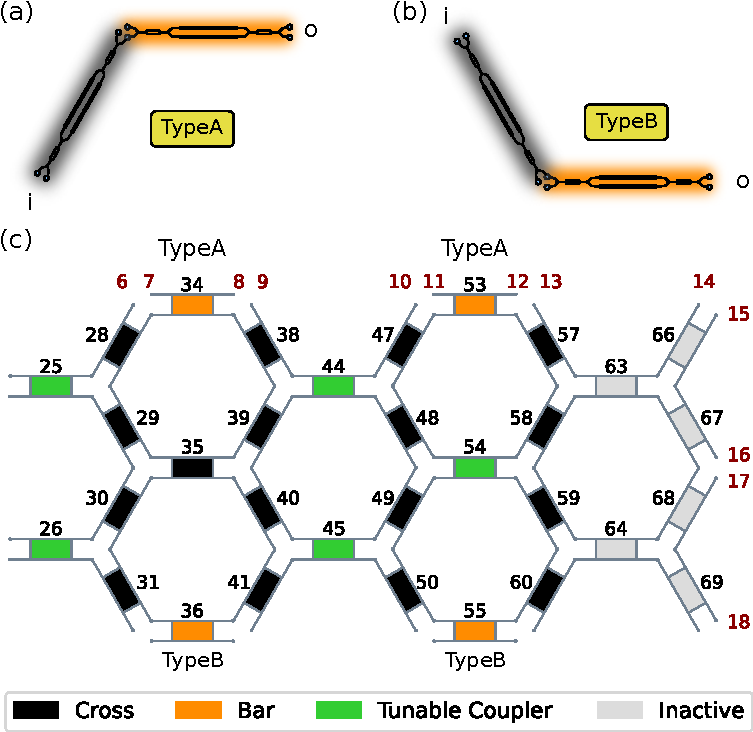
\includegraphics{figures/ch4-pucs_type_a_b.pdf}
	\caption{
		Pairs of PUCs of two types (A and B) allow having a complete implementation of a rectangular mesh on the hexagonal core.
	}\label{fig:ch4-pucs_type_a_b}
\end{figure}

Notice that Equations~\eqref{eq:map_ff_hex_3}, \eqref{eq:map_ff_hex_a_1} and \eqref{eq:map_ff_hex_b_1} are all the same.
This makes sense if we remember that in the three cases the PUCs have to be configured in a cross state without a cross phase to represent a single photonic wire.
Therefore, we can consider \eqref{eq:map_ff_hex_3} to be general for this scenario.

To sum up, if we want to map an arbitrary rectangular architecture to its hexagonal equivalent, we will need to convert the phases obtained using the Clements/Reck decomposition according to the equations presented above.
Equations~\eqref{eq:map_ff_hex_1} and \eqref{eq:map_ff_hex_2} will need to be used for all the MZI phases in the feedforward circuit.
For all the auxiliary PUCs, Equations~\eqref{eq:map_ff_hex_3}, \eqref{eq:map_ff_hex_a_2} and \eqref{eq:map_ff_hex_b_2} need to be used depending on the PUC state and/or the type of connection.

% section Feedforward to Hexagonal translation (end)
\section{Calibration of rectangular feedforward circuit}\label{sec:ff_calibration} % (fold)

Previous publications show that a calibration routine is needed to effectively perform matrix operation on MZI-based unitary operators \cite{alexiev_calibrating_2021}.
Although the hexagonal meshes, subject of this work, have already gone through the calibration process covered in Section~\ref{sub:calibration}, this process only took into account the parasitic phases between the PUC arms.
However, in the case of circuits like the Clements circuit, another set of passive phases must be taken into account: the interconnection between PUCs.
The results previously published in \cite{perez-lopez_general-purpose_2024, on_programmable_2024} already pointed that whenever a recirculating interferometric structure was implemented on the hexagonal arrays a phase mismatch could be deduced from their spectral response.
The study of these occurrences led us to the proposal of a new non-ideal model for a PUC that can account for this and can be used as a basis for a complementary calibration routine for such structures.

\subsection{Updated PUC model}\label{sub:updated_puc_model} % (fold)

\begin{figure}[t]
	\begin{center}
		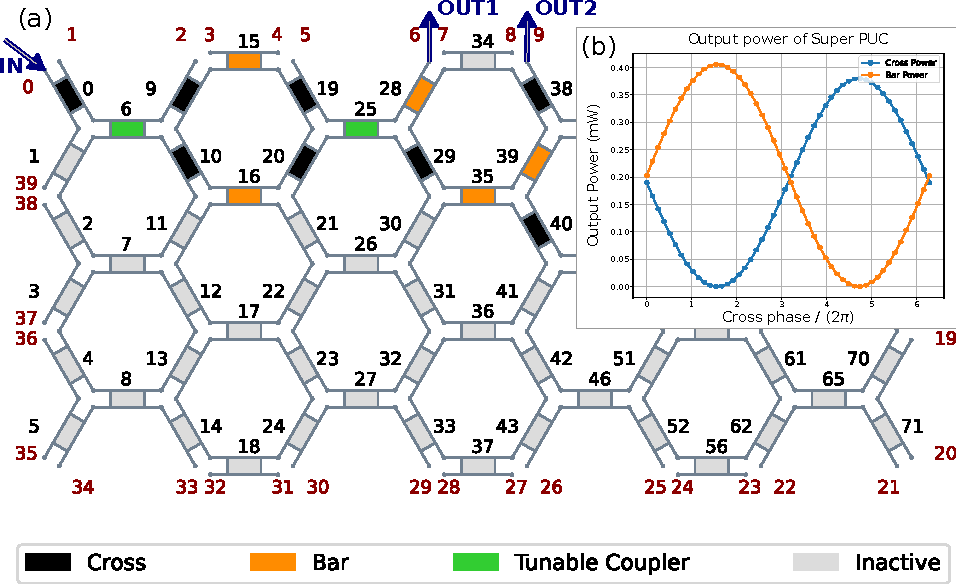
\includegraphics{figures/ch4-superpuc.pdf}
	\end{center}
	\caption{MZI instantiated in the hexagonal mesh (left) and its measured output power for different cavity
		phases}\label{fig:ch4-superpuc}
\end{figure}

To understand the effect of parasitic interconnection phases in hexagonal cells we start by studying the simplest case: the balanced MZI circuit, i.e., a circuit composed by the 6 PUCs surrounding a hexagonal cell as presented in Figure~\ref{fig:ch4-superpuc}.
The phase difference between the upper and lower arms of this MZI should in theory be zero and therefore the MZI circuit should be in cross state by default.
As covered in Section~\ref{sub:calibration}, using \lstinline|set_coupling_factor_phase|, each composing PUC can be programmed to a have a 0 cross-phase, therefore the compound circuit should behave as an ideal MZI.
However, what we observe in Figure~\ref{fig:ch4-superpuc} is that the circuit is configured as if an effective phase shift had been applied to one of its arms when that's not the case.
This led us to conclude that a parasitic phase shift is introduced at the chip level.
The same behavior has been reported in other structures such as rings and filters.

\begin{figure}
	\begin{center}
		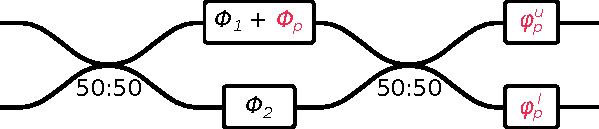
\includegraphics{figures/ch4-pucmodel.pdf}
	\end{center}
	\caption{Proposed new model of non-ideal PUC}\label{fig:ch4-pucmodel}
\end{figure}

To better explain this phenomenon we have proposed the new non-ideal PUC model depicted in Figure~\ref{fig:ch4-pucmodel}.
In addition to the internal passive phase shift within the PUC arms we now also consider the shift introduced by the silicon waveguide interconnections between PUCs.
The effects of these spurious phases are clearly observed in phase-dependent circuits such as filters, interferometric operators but are also completely masked by the photodetectors in amplitude-only applications such as switches and beamsplitters.
Therefore, for coherent applications we must perform an additional calibration routine.
To sum up, the routine in Section~\ref{sub:calibration_of_puc_cells} compensates \(\phi_p\) within the PUC and the passive phases between PUCs \(\phi^u_p\) and \(\phi^l_p\) must be characterized using an additional routine.

% subsection Updated PUC model (end)
\subsection{Calibration of PUC cells}\label{sub:calibration_of_puc_cells} % (fold)

Finding out the values of \(\phi^u_p\) and \(\phi^l_p\) for the entire mesh is a nontrivial task and a discussion of its possible acquisition has been reserved for Section~\ref{sub:circuit_aware_calibration}.
Here we limit our study to a lumped element simplification that can be used for the case of multi-port interferometers.
Considering the phase introduced in the connection between PUCs we know that the phases introduced in the lower and upper arms are not the same.
The experimental results indicate that the phase difference between the arms is not zero.
Following the new PUC model we can express this parasitic phase difference this way:
\begin{equation}
	\phi^l_{up} = \phi^{(6,9)} + \phi^{(9,15)} + \phi^{(15,19)} + \phi^{(19,25)}
	\label{eq:ch4-superpuc_up}
\end{equation}

\begin{equation}
	\phi^l_{lo} = \phi^{(6,10)} + \phi^{(10,16)} + \phi^{(16,20)} + \phi^{(20,26)}
	\label{eq:ch4-superpuc_lo}
\end{equation}
where \eqref{eq:ch4-superpuc_up} and \eqref{eq:ch4-superpuc_lo} correspond to the total lumped (\(l\)) parasitic phase on each arm, respectively.
Therefore, to calibrate this MZI circuit, we need to compensate the equivalent lumped circuit phase \(\phi^l_{MZI}\) \eqref{eq:ch4-superpuc_lumped} given by the difference between upper and lower arms:

\begin{equation}
	\phi^l_{MZI} = \phi^l_{up} - \phi^l_{lo}.
	\label{eq:ch4-superpuc_lumped}
\end{equation}

This means that if we want to calibrate an MZI circuit we need to apply \(-\phi^l_{MZI}\) as a compensation cross-phase to a PUC in the upper arm of the cell.
Note that, as shown in Figure~\ref{fig:ch4-superpuc_hex}, the use the lumped model simplification removes the need to characterize the values \(\phi^u_p\) and \(\phi^l_p\) of each PUC.
If From here onwards we will drop the \(l\) superscript and consider all parasitic phases lumped unless otherwise stated.
This phase value must be compensated for each cell in the mesh so that a synthesized MZI circuit will be set to cross state.
Therefore, in hardware, to find the compensating phase, we use a gradient descent optimizer \cite{noauthor_optimization_nodate} to find the phase that maximizes the cross power.
We use an optimizer instead of a phase sweep as it converged more quickly on the right calibration phase and this time we don't need to characterize the full MZI response as reported in Section~\ref{sub:calibration}.
This phase could then be added to any PUC that forms the upper/lower arms.
The process was then automated and repeated for all the cells in the mesh (see Figure~\ref{fig:ch4-hex_cells}).

\begin{figure}[h]
	\begin{center}
		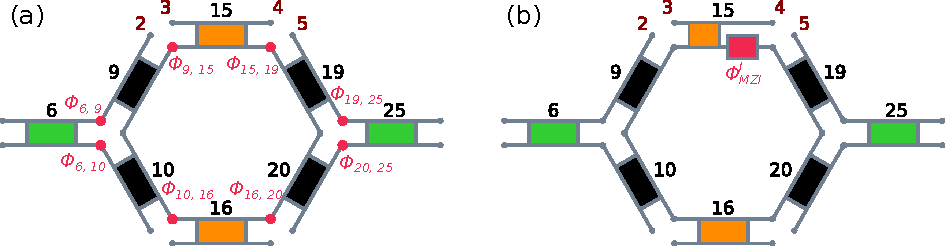
\includegraphics{figures/ch4-super_puc_hex.pdf}
	\end{center}
	\caption{Non-ideal junction phases added to hexagonal cells (a) and their corresponding lumped model (b)}\label{fig:ch4-superpuc_hex}
\end{figure}

\begin{figure}
	\begin{center}
		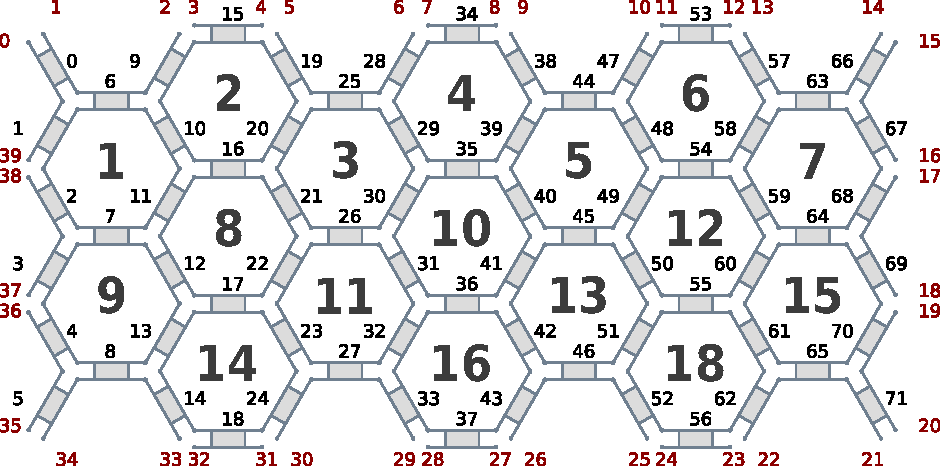
\includegraphics{figures/ch4-hex_cells.pdf}
	\end{center}
	\caption{Numbered MZI cells in the iPronics hexagonal core}\label{fig:ch4-hex_cells}
\end{figure}

% subsection Calibration of PUC cells (end)

\subsection{Calibration of feedforward operators}\label{sub:calibration_of_feedforward_operators} % (fold)

\begin{figure}
	\begin{center}
		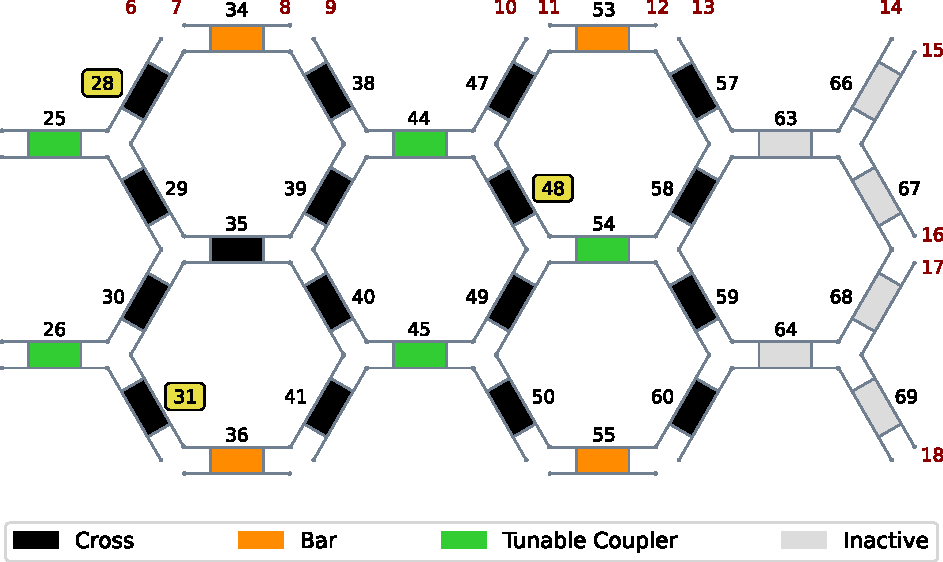
\includegraphics{figures/ch4-superpuc_compensation.pdf}
	\end{center}
	\caption{Synthesized feedforward mesh with PUCs where the compensation is applied as a cross-phase delta
		(yellow)}\label{fig:ch4-superpuc_compensation}
\end{figure}

The calibration presented in Section~\ref{sub:calibration_of_puc_cells} corrects the lumped passive phase inside each MZI circuit.
To calibrate the multiport interferometer (i.e., the Clements mesh), we can use the phases obtained from the previous MZI calibration.
In this kind of feedforward mesh the cavities are coupled so that we should be careful when choosing where we compensate the passive phases of each individual MZI.
The most effective way to do that is to compensate the phases in PUCs that are not shared between hexagonal cavities.
For example, in Figure~\ref{fig:ch4-superpuc_compensation} to calibrate a 4-port unitary operator we can apply the compensation phases to PUCs 28, 31 and 48 to calibrate the MZIs placed on hex cells 4, 10 and 5, respectively (refer to Fig.~\ref{fig:ch4-hex_cells}).
There might be scenarios for which isolated compensation is not possible.
In those cases we can compensate the cells taking into account the overlap between paths.
For example, suppose we are restricted to compensate with PUCs 35, 40 and 49 (chosen for illustrative purposes).
In this scenario the phases applied to calibrate the whole Clements circuit are
\begin{equation}
	\begin{aligned}
		\phi^{(35)} & = -\phi^{(4)}_{MZI}                                        \\
		\phi^{(40)} & = \phi^{(10)}_{MZI} + \phi^{(4)}_{MZI}                     \\
		\phi^{(49)} & = -\phi^{(5)}_{MZI} - \phi^{(10)}_{MZI} - \phi^{(4)}_{MZI}
	\end{aligned}
	\label{eq:ch4-clements_calib_complex}
\end{equation}
where the phases on the left-hand side correspond to the effective cross-phase applied to an individual PUC and the phases on the right-hand side correspond to each MZI cell parasitic phase.
With these calibration phases, the feedforward circuit's phase response will now be error free.

% subsection Calibration of feedforward operators (end)
% section Calibration of synthesized feedforward circuit (end)

\section{Feedforward operator}\label{sec:feedforward_operator} % (fold)

\subsection{Feedforward operator in code}\label{sub:feedforward_operator_in_code} % (fold)

\begin{lstlisting}[caption={A 3x3 Feedforward operator instance in hexagonal mesh}, label={lst:ch4-definition}]
	feedforward = smart.feedforward_operator(dim=3, puc_0=0)
	smart.load_feedforward_config(feedforward)
	core_monitor.plot_mesh_status()
\end{lstlisting}

Once these calibration phases have been loaded to the feedforward operator circuit, the equivalent Hexagonal-Clements decomposition phases presented in Section~\ref{sec:feedforward_to_hexagonal_translation} can be applied to the circuit PUCs.
Here we cover the implementation of such operator as a logical element that can be synthesized on the first-generation Smartlight hexagonal core through a simple set of Python instructions.
Listing~\ref{lst:ch4-definition} shows the instructions needed to instantiate a logical feedforward circuit.
First, we generate the feedforward operator object using \lstinline|feedforward_operator(dim, puc_0)|.
By specifying the input parameter \lstinline|dim|, we have flexibility to select the dimension of our feedforward operator.
Given the specifications of the first-generation Smartlight mesh, we are capable of creating feedforward operators with dimensions ranging from 2 to 6.
Moreover, we can also choose where to place the feedforward operator through the \lstinline|puc_0| parameter.
This location is indicated with the PUC in the upper left corner of the operator, in which the lower port is the one used to input the signal.
After creating the operator object, one can integrate it into the mesh by employing \lstinline|load_feedforward_config()| and providing the previously generated operator as the input parameter.

\begin{figure}
	\begin{center}
		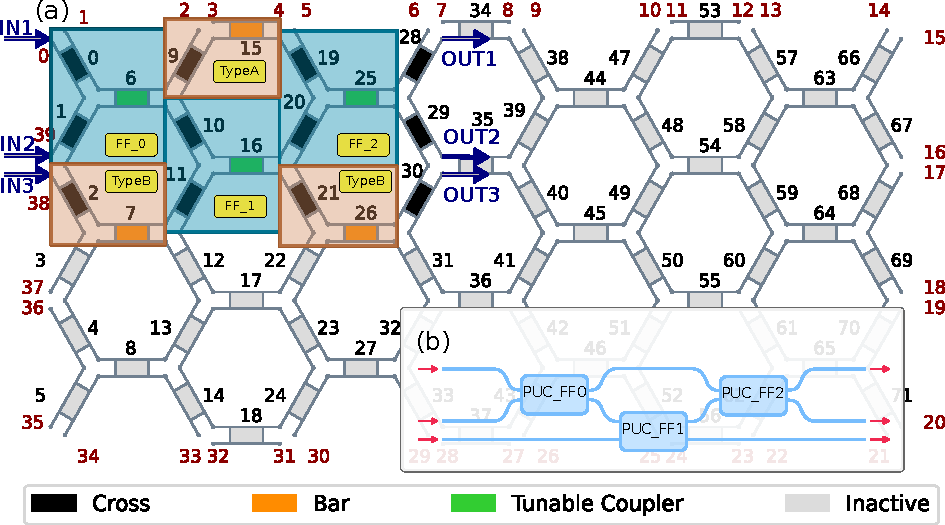
\includegraphics{figures/ch4-ff_in_hex.pdf}
	\end{center}
	\caption{(a) A 3-by-3 Feedforward operator instance with all its compoosing elements implemented in the hexagonal mesh. (b) equivalent Clements circuit of size \(N=3\).}\label{fig:ch4-ff_in_hex}
\end{figure}

We can always access to the feedforward operator created using the \lstinline|puc_config| attribute as shown in Listing~\ref{lst:ch4-puc-translation}.
As we have seen in previous sections, the configuration of each PUC can be provided by two distinct methods:

\begin{enumerate}
	\item \lstinline|set_coupling_factor_phase()|: Sets a coupling factor $k$ and a cross phase $\Delta$
	\item  \lstinline|set_driven_phases()|: Sets directly the phases $\phi_{lo}$ and $\phi_{up}$
\end{enumerate}

In this case, we will use the second option to load the phases derived in Section~\ref{sec:feedforward_to_hexagonal_translation}.
As explained in that section, a trilattice is conformed by three PUCs with different behaviors: a tunable coupler, a phase shifter and a photonic wire.
Therefore, each instance of \lstinline|FeedForwardOperator| is associated with three sets of PUCs, each with their respective functionalities as shown in Listing~\ref{lst:ch4-puc-translation} and Figure~\ref{fig:ch4-ff_in_hex}.

\begin{lstlisting}[caption={Equivalence between hexagonal PUCs and feedforward ones},
label={lst:ch4-puc-translation}]
	# Access to the puc configuration
	puc_config = feedforward.puc_config
	# Consult which PUCs are tunable couplers
	tunable_couplers = feedforward.coupler_pucs
	# Consult which PUCs are tunable phase shifters
	phase_shifters = feedforward.phase_shifters
	print("PUCs acting as tunable coupler are:", tunable_couplers)
	>>> PUCs acting as tunable coupler are: [6, 16, 25]
	print("PUCs acting as phase shifter are:", phase_shifters)
	>>> PUCs acting as phase shifter are: [0, 10, 19]
\end{lstlisting}

% subsection Feedforward operator in code (end)
\subsection{Implementation of arbitrary unitary matrices}\label{sub:implementation_of_arbitrary_unitary_matrices} % (fold)

%%%%%% puo paper
Based on the aforementioned rationale, we have implemented these operators as logical parametric units that can be placed on different positions of the first-generation Smartlight's mesh \cite{perez-lopez_general-purpose_2024}.
Listing~\ref{lst:ch4-instruction} presents the instruction set we have developed to instantiate unitary operators on a hexagonal-based chip architecture.
The parametric and floating nature of the operator is presented in line 3, where the developer inputs the dimension \lstinline|N| of the logical unit and its location \lstinline|puc_0| on the hexagonal grid, respectively.
The dimensions of the hexagonal mesh constrain both parameters.
The current chip architecture can support operators up to a maximum size of $N = 6$.
The instruction set, however, is agnostic of this constraint and supports larger and smaller meshes.
Line 5 shows how a unitary matrix $U$ is loaded to the chip.
This instruction performs the mathematical decomposition and translation from Clements-based phases to their hexagonal equivalent.
Line 7 then loads this new phase configuration on the logical operator, considering calibration data from its location on the hexagonal grid, to end up with the unitary implemented on hardware.
By following this procedure, logical unitary operators can be deployed on different mesh locations and be accessed through the system I/O ports or connected to other subcircuits on the mesh in a place-and-route fashion for further application development.
Note that because of this floating feature any of the mesh I/O ports or the internal mesh node can be used as inputs to the parametric unitary operator.

\begin{lstlisting}[caption={Basic instruction set needed to implement matrix operators on the first-generation Smartlight}, label={lst:ch4-instruction}]
	from smartlight import feedforward_operator
	# Create operator
	ff = feedforward_operator(dim=N, puc_0=38)
	# Load matrix to the operator
	ff.load_unitary_matrix(U)
	# Load phase configuration into the mesh
	hex_mesh.load_feedforward_config(ff)
\end{lstlisting}

To illustrate this procedure, let's review the implementation of a 1-by-3 beamsplitter.
First, we define the transfer matrix presented in Eq.~\eqref{eq:beamsplitter}

\begin{equation}
	\label{eq:beamsplitter}
	T_{BS} = \frac{1}{\sqrt{3}} \begin{bmatrix}
		1 & 1            & -1          \\
		1 & e^{i2\pi/3}  & e^{i4\pi/3} \\
		1 & e^{-i4\pi/3} & e^{i8\pi/3}
	\end{bmatrix}
\end{equation}

With \(I = \begin{bmatrix} 1 & 0 & 0 \end{bmatrix}^T\) acting as normalized input for this particular case in which the internal laser (\(P=5\)~dBm) is connected to the first unitary operator port.
Eq.~\eqref{eq:beamsplitter} is implemented in hardware using the code in Listing~\ref{lst:ch4-beamsplitter}.

\begin{lstlisting}[caption={Implementation of a three-way beamsplitter using a Feedforward operator},
label={lst:ch4-beamsplitter}]
	# T_BS: Transfer matrix of a 1-by-3 beamsplitter
	smart.reset_mesh()
	# Create the feedforward operator
	feedforward = smart.feedforward_operator(dim=3, puc_0=38)
	feedforward.load_unitary_matrix(T_BS)
	# Load the feedforward configuration into the mesh
	smart.load_feedforward_config(feedforward)
	# Define input path to operator
	path = [
		(0, ["x", 0]),
		(6, ["=", 0]),
		(9, ["x", 0]),
		(15, ["=", 0]),
		(19, ["x", 0]),
		(25, ["=", 0]),
		(28, ["x", 0]),
		(34, ["=", 0]),
	]
	smart.set_coupling_factor_phase(path)
	core_monitor.plot_mesh_status()
\end{lstlisting}

\begin{figure}
	\begin{center}
		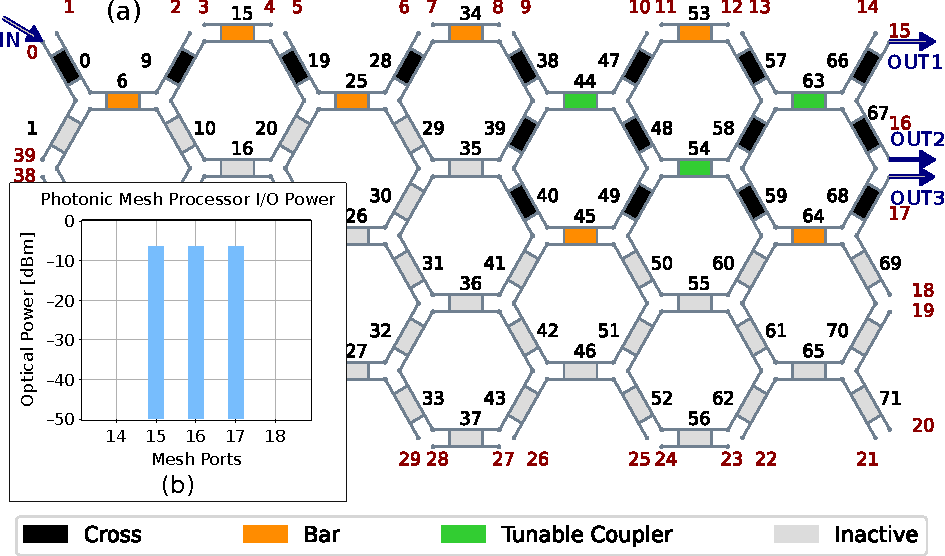
\includegraphics{figures/ch4-3split_mema.pdf}
	\end{center}
	\caption{(a) Implementation of three-way beamsplitter in the hexagonal mesh using a 3-by-3  Feedforward
		operator.
		In (b) the output power distribution observed by the MEMA monitor.
	}\label{fig:ch4-3split} \end{figure}

The resulting circuit is presented in Figure~\ref{fig:ch4-3split}, where one can observe the unitary operator spanning from PUC 38 and with its outputs directly connected to the mesh output ports for power monitoring.
Additionally, an optical interconnect has been created to connect one input of the operator to the laser at system port 0.
By plotting the output distribution using the power monitor, we can see that the power has been equally distributed among the three outputs with a split of -4.77 dB corresponding to \(\frac{1}{3}\) (see Figure~\ref{fig:ch4-3split}(b)).

In the following section, we conclude this chapter by covering some applications of interest for the telecom/datacom community involving unitary operators of different sizes.
% subsection Implementation of arbitrary unitary matrices (end)
%-------------------------------------------------- Hybrids Section -------------------------------------------------------%
\section{Optical hybrids for coherent links}
% - 'Experiment explanation':
% - Matrix Equations
\begin{figure}[t!]
	\centering
	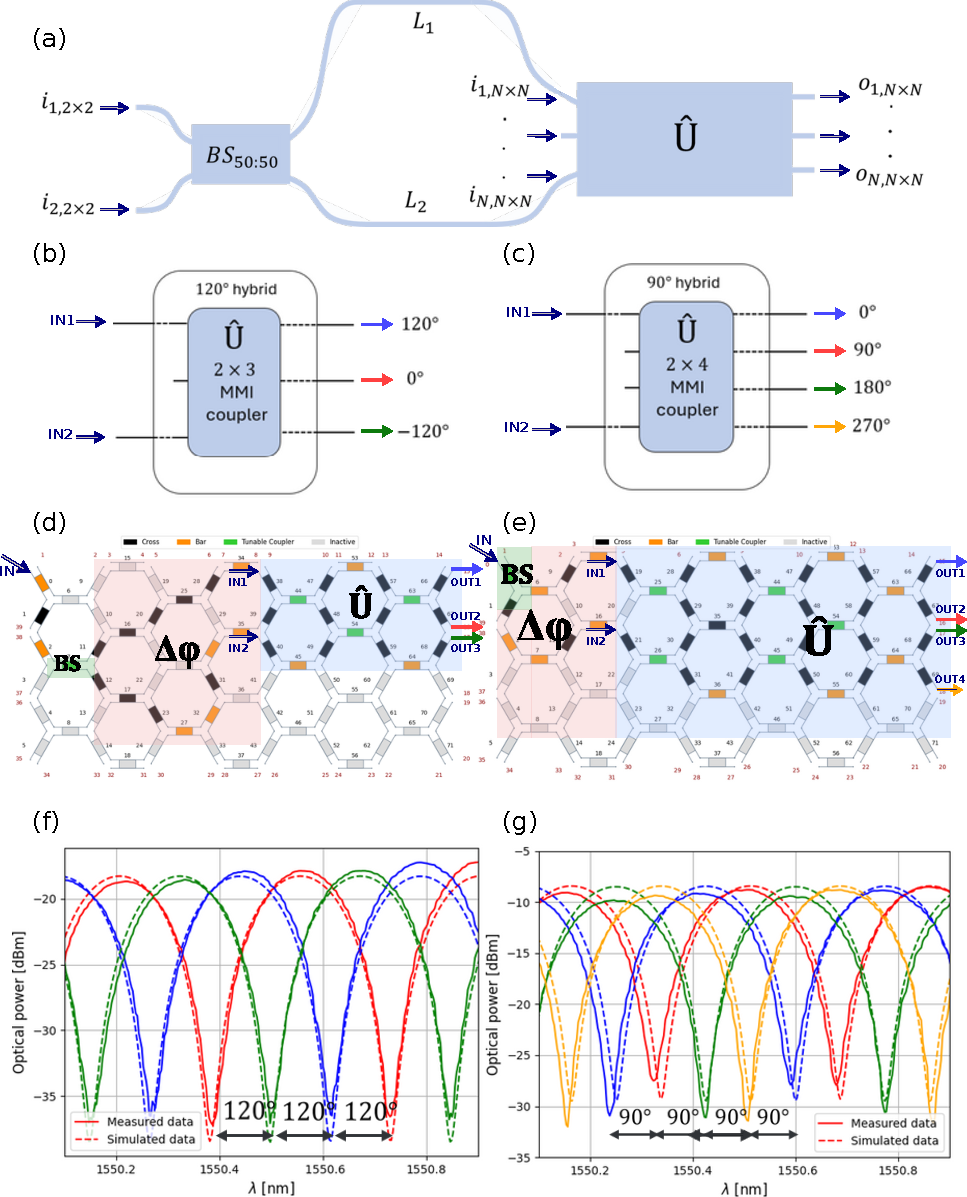
\includegraphics{figures/ch4-hybrids.pdf}
	\caption{Photonic circuit (a) used to demonstrate the 120$^o$ (b) and 90$^o$ (c) hybrid functionality of a logical unitary operator synthesized on hexagonal chip architecture (d-e).
		Optical power measured at the operators' outputs, shown in different colors, for the 120$^o$ (f) and 90$^o$ (g) hybrids with their resulting phase difference inferred from the FSR.
	}
	\label{fig:hybrids}
\end{figure}

Coherent transceivers are ubiquitous elements of telecom links.
Their use within data centers has only been limited by the lower price and power consumption of their intensity-modulation direct-detection (IM-DD) counterparts.
The progressive introduction of coherent technology in data centers is predicted to grow during the next decade to satisfy data rate increasing demands.
\cite{maharry_first_2022}.
A key element of these devices on the reception side is a hybrid capable of mixing the incoming signal with the local oscillator (LO) and producing a combined output with both signals out of phase by a certain $\Delta\phi$ angle between them.
The mathematical representation of this operation is given by Eq.~\eqref{eq:mmi3} for 120$^o$ and Eq.~\eqref{eq:mmi4} for 90$^o$, which in turn corresponds to the transfer functions of 3x3 and 4x4 MMIs, respectively.
\begin{equation}\label{eq:mmi3}
	U = \frac{1}{\sqrt{3}}
	\begin{bmatrix}
		-e^{-i2\pi/3} & e^{-i2\pi/3} & -1             \\
		e^{-i2\pi/3}  & -1           & e^{-i2\pi/3}   \\
		-1            & e^{-i2\pi/3} & - e^{-i2\pi/3}
	\end{bmatrix}
\end{equation}

\begin{equation}\label{eq:mmi4}
	U = \frac{1}{\sqrt{4}}
	\begin{bmatrix}
		e^{i\pi}    & e^{-i\pi/4} & e^{i3\pi/4} & e^{i\pi}    \\
		e^{-i\pi/4} & e^{i\pi}    & e^{i\pi}    & e^{i3\pi/4} \\
		e^{i3\pi/4} & e^{i\pi}    & e^{i\pi}    & e^{i7\pi/4} \\
		e^{i\pi}    & e^{i3\pi/4} & e^{i7\pi/4} & e^{i\pi}    \\
	\end{bmatrix}
\end{equation}
Since Equations~\eqref{eq:mmi3}, \eqref{eq:mmi4} refer to linear systems, they can easily be implemented on a hexagonal mesh using the logical unitary operator introduced in the previous section.
To demonstrate the hybrid operation, the circuit in Fig.~\ref{fig:hybrids}(a) is synthesized on the mesh.
Here, the injected light is split using a 3-dB coupler, and an asymmetric MZI structure is connected to the hybrid's input.
Insets (b) and (d) show the implementation when the operator tested is a 120$^o$ hybrid ($U = $ Eq.~\eqref{eq:mmi3}), and insets (c) and (e) show the 90$^o$ case ($U = $Eq.~\eqref{eq:mmi4}).
In (f) and (g), we observe the power measured at the outputs of the operator for the two cases.
The relative phase differences are determined using the $\Delta\phi/\Delta\lambda = 2\pi/FSR$.
The solid lines represent the experimental results, and the dotted ones are the simulated ones.
These traces closely match each other and replicate the ones of previously reported dedicated 120$^o$ and 90$^o$ hybrids \cite{saber_demonstration_2018, yu_high-performance_2020, reyes-iglesias_high-performance_2012}, thus demonstrating that the operator can deploy both functionalities using the same hardware.

%-------------------------------------------------- Multicast Section -------------------------------------------------------%
\section{The WDM multicast switch}

%- Matrix Equations
%- Experiment explanation
%- Application in WDM links

Multicast switches (MCS) are key elements of existing ROADM solutions in which the combination of wavelength selective switches (WSS), tunable filters, and optical amplifiers alongside the MCS enable the so-called colorless, directionless, and contentionless (CDC) operation to meet current internet requirements \cite{watanabe_multicast_2014,yang_low-cost_2017}.
The MCS performs the split and combines operations of different wavelength-carrier signals as shown in Fig.~\ref{fig:multicast}(a).
This linear operation can be represented by Eq.~\eqref{eq:dft}, which corresponds to a DFT operator.
Since the inputs to the operator have different wavelengths, the DFT phase shifts don't have any effect, and $U$ acts as a split-and-combine operator.

\begin{equation}\label{eq:dft}
	U = \frac{1}{\sqrt{6}}
	\begin{bmatrix}
		1 & 1           & 1           & 1  & 1           & 1           \\
		1 & e^{i\pi/3}  & e^{2i\pi/3} & -1 & e^{i4\pi/3} & e^{i5\pi/3} \\
		1 & e^{2i\pi/3} & e^{i4\pi/3} & 1  & e^{i2\pi/3} & e^{i4\pi/3} \\
		1 & -1          & 1           & -1 & 1           & -1          \\
		1 & e^{i4\pi/3} & e^{2i\pi/3} & 1  & e^{i4\pi/3} & e^{i2\pi/3} \\
		1 & e^{i5\pi/3} & e^{i4\pi/3} & -1 & e^{i2\pi/3} & e^{i\pi/3}  \\
	\end{bmatrix}
\end{equation}

To test this operation mode, we have created an $N=6$ logical operator, loaded the DFT matrix to it, and connected its inputs to six lasers with different wavelengths, see Fig.~\ref{fig:multicast}(b).
As seen by a spectrum analyzer, the output from this system is shown in (c), where the spectra of the six input carriers are shown next to the spectrum of output 1.
The latter contains a signal with all six wavelength components combined and powers of -7.78~dB (i.e., a $1/6$ split) with respect to the input laser peak powers, as expected in a practical MCS system.
Note that since this operator implements \eqref{eq:dft} it could also be used to demonstrate the costly DFT operation if same-wavelength inputs and coherent detection were used.

\begin{figure}[h]
	\centering
	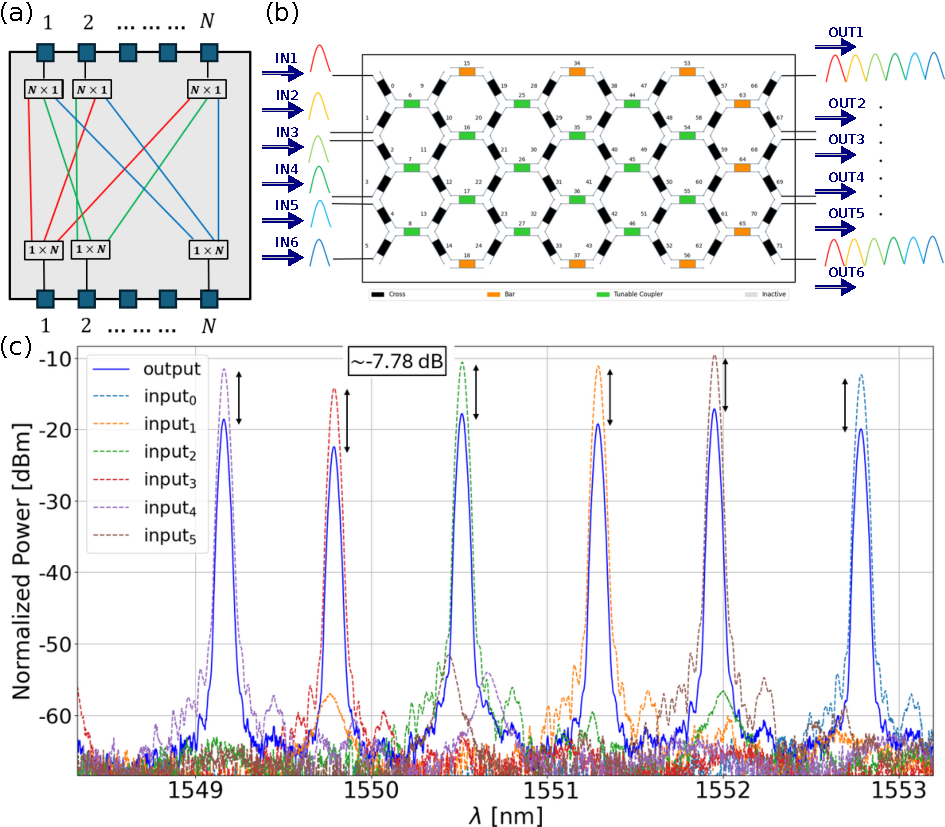
\includegraphics{figures/ch4-mcs.pdf}
	\caption{Schematic (a) of a multicast switch used in ROADMs to split and combine different wavelength carriers and its implementation on the reconfigurable mesh (b) using a 6-by-6 unitary operator.
		The measured spectra in (c) contain the resulting split-and-mixed signal at output port 1-6 and the incoming carriers (other colors).
	}
	\label{fig:multicast}
\end{figure}

%-------------------------------------------------- OCS Section -------------------------------------------------------%
%\section{Optical circuit switching}
%- Matrix Equations
%Eq.~\eqref{eq:switch}

%\begin{equation}\label{eq:switch}
%U=
%\begin{bmatrix}
%0 & 0 & 0  & 1 & 0 & 0 \\
%0 & 0 & 0  & 0 & 1 & 0 \\
%0 & 0 & 0  & 1 & 0 & 1 \\
%1 & 0 & 0  & 0 & 0 & 0 \\
%0 & 1 & 0  & 0 & 0 & 0 \\
%0 & 0 & 1  & 0 & 0 & 0 \\
%\end{bmatrix}
%\end{equation}
%- Experiment explanation
%- Application in DC links

%\lipsum[3]  
%-------------------------------------------------- Conclusions Section -------------------------------------------------------%
\section{Conclusions}
This chapter has introduced the concept of logical unitary operators that can be deployed on a reconfigurable hexagonal chip architecture using a place and route fashion as sub circuits or standalone elements using a short set of code instructions.
We have explored and experimentally demonstrated different applications of such operators using the iPronics first-generation Smartlight platform, including optical hybrids for coherent transceivers and a multicast switch for ROADMs, using different operator sizes.
The applications, however, are far more extensive than this small subset, as linear operations lie at the heart of several optical systems.
With this contribution, we aim to provide the photonics community with a tool that enables and fosters the fast development and deployment of new optical solutions, effectively and flexibly addressing the critical need for innovative, reconfigurable, and mass-manufacturable semiconductor solutions that can fulfil the growing demand for faster and cheaper data transmission.
% section Feedforward operator (end)
% chapter Universal Unitary Operators (end)


% Author: David Sanchez-Jacome

\chapter{Discussion and conclusions}\label{chap:discussion_and_conclusions} % (fold)

\section{Thermal crosstalk}\label{sec:thermal_crosstalk} % (fold)

\begin{figure}
	\begin{center}
		\includegraphics{figures/ch5-thermal_setup.pdf}
	\end{center}
	\caption{Setup of experiment used to measure the effect of thermal crosstalk on the iPronics chips.}\label{fig:ch5-thermal_setup}
\end{figure}

Thermal crosstalk is a major concern in silicon photonic integrated circuits (PICs) due to the high temperature sensitivity of photonic devices like Mach-Zehnder interferometers and microring resonators, which rely on precise refractive index control.
In densely integrated PICs, heat generated by thermal tuners can unintentionally affect neighboring components, leading to phase errors, wavelength shifts, and degraded performance.
Programmable PICs often pack numerous optical components and heaters (e.g., thermal tuners) into a compact area to achieve complex functionality.
Therefore, the proximity of these components means heat generated by one heater can unintentionally affect neighboring devices, causing unpredictable and undesired changes in their performance.
This issue increases power consumption, complicates thermal management, and reduces system stability and reliability, particularly as PICs scale in complexity.
To mitigate thermal crosstalk, strategies such as thermal isolation, active cooling, advanced control algorithms, and non-thermal tuning methods are explored to improve energy efficiency and ensure robust performance.
In particular, a silicon photonic platform implementing a set of underetched phase actuators optimized to contain the heat from the resistor within a small volume of air, leads to chips more resilient to thermal crosstalk aggression \cite{liu_thermo-optic_2022}.
Nevertheless, this design doesn't make the platform completely immune to this type of crosstalk.

During this thesis we have studied the effects of this thermal nonideality in the developed silicon photonic chips using underetch technology \cite{cem_thermal_2023, teofilovic_thermal_2024}.
To perform this study we synthesized a Micro Ring Resonator (MRR) in the mesh as this structure is very sensitive to thermal fluctuations (shown in Figure~\ref{fig:ch5-thermal_setup}).
The standard response of the MRR corresponds to a series of spectral notches occurring at wavelengths where the resonance condition is met:
\begin{equation}
	m\lambda = n_{eff}2\pi r
	\label{eq:ch5-ring_eq}
\end{equation}
where \(m\) is an integer value, \(n_{eff}\) is the effective group index of the propagating mode and \(r\) corresponds to the ring radius.
We then drove the thermal actuators of neighboring PUCs with high currents until the effect of thermal deviation was observed in the spectral response as depicted in Figure~\ref{fig:ch5-thermal_comp_ring1}.

\begin{figure}
	\begin{center}
		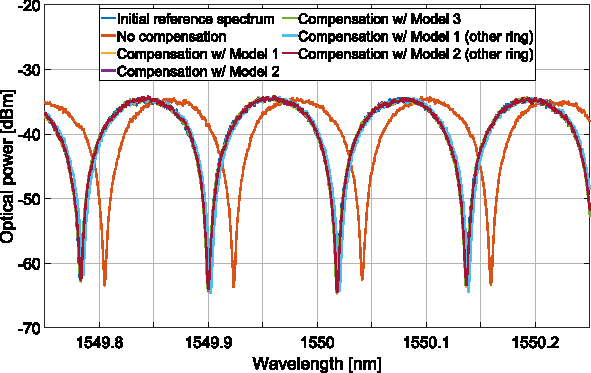
\includegraphics{figures/ch5-thermal_comp_ring1.pdf}
	\end{center}
	\caption{Response of an ORR circuit before and after the effects of severe thermal crosstalk and three proposed approaches to mitigate it.}\label{fig:ch5-thermal_comp_ring1}
\end{figure}

We observe that in the presence of this crosstalk aggressor the response of the circuit moves to the right as the effective refractive index \(n_{eff}\) increases with the temperature.
This leads the notches to shift to higher wavelengths while keeping the FSR constant.
Recall that this happened on a thermally controlled chip with isolated phase shifters, meaning that this effect is completely spurious.

If this undesired effect is to be mitigated, it has to be modeled first.
We considered two models: one based on the thermal diffusion of heat in a bulk material represented by a weighted summation of the phases \(\phi\) with the weight depending on
the distance \(d\) from the heat source \cite{jacques_optimization_2019} given by
\begin{equation}
	\Delta \lambda = \sum_i \left( p_1 e^{-p_2 d_i} + p_3 d_i + p_4 \right) \phi_i
	\label{eq:ch5-thermal_exp_fit}
\end{equation}
and another model based on a standard ridge regression that considers the driving phases of all the aggressor PUCs weighted by a train parameter
\begin{equation}
	\Delta \lambda = \sum_i a_i \phi_i + b
	\label{eq:ch5-thermal_ml_regressor}
\end{equation}
where in both cases \(p_i\), \(a_i\) and \(b\) are fitting parameters and where the regularization parameter was optimized using five-fold cross validation.

Both models were trained to minimize the root-mean squared error (RMSE) between the experimentally measured and the predicted wavelength shifts.
A large dataset is obtained measuring several neighboring PUCs driving currents and their subsequent phase shift: 80\% of the data was used for training and 20\% for testing.

\begin{figure}
	\begin{center}
		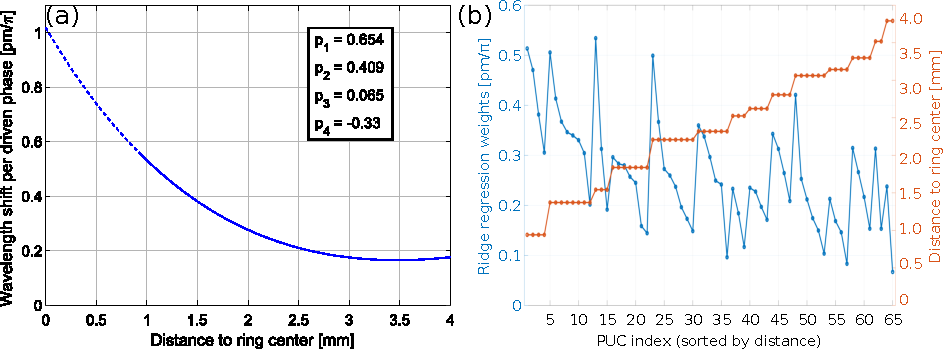
\includegraphics{figures/ch5-thermal_diffusion_correlation.pdf}
	\end{center}
	\caption{(a) Analytical  exponential decay model after fitting with optimal parameters shown in the box. (b) Weights found by ridge regression plotted alongside the distance to ring center for each PUC.
		The two are inversely correlated with \(\rho = -0.53\).
	}\label{fig:ch5-thermal_correlation}
\end{figure}

The analytical and data-driven models achieved 0.55 and 0.43 pm RMSEs, which resulted in testing RMSEs of 0.55 and 0.50 pm for, respectively.
Note that former model has four degrees of freedom, whereas the later 67 (66 weights and 1 bias).
The evolution of \(\Delta \lambda\) with distance is shown in Figure~\ref{fig:ch5-thermal_correlation} for the analytical model.
A major advantage of this model is that it can extrapolate to PUCs not considered in the experiment, providing valuable insight for future chip designs with more densely packed PUCs.
The weights found for the regressor model are presented in Figure~\ref{fig:ch5-thermal_correlation} where, although distance information was not fed to the regressor we observe an inverse correlation between the trained value and the distance to the regressor.
This method represents a black box approach that can be used when no information about the chip layout is available.

Finally, in order to validate the models created, we drove the 22 neighboring PUCs' cross phases (Fig.~\ref{fig:ch5-thermal_setup}) from \(0\) to \(2\pi\) and based on the models' predicted wavelength shift we counteracted it by applying the complementary phase shift \(\phi_c = 2 \pi(1-\frac{\Delta \lambda}{FSR})\) to one of the ring's actuators.
After the compensation, the initial and compensated notches were measured to be within \pm 0.5 pm.
Similar results were obtained when compensating a ring's shift using another ring's model as detailed in \cite{teofilovic_thermal_2024}.
This work paves the way to predicting and correcting the effects of severe thermal crosstalk in densely integrated PICs providing developers with principles to create lookup-table-based or active control loops to ensure reliability across chips for phase sensitive applications.
% section Thermal crosstalk (end)
\section{Optical computing}\label{sec:optical_computing} % (fold)

\begin{figure}
	\begin{center}
		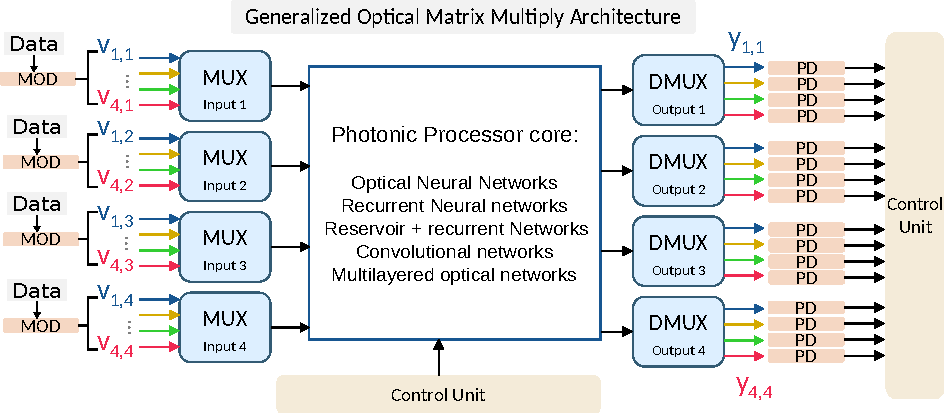
\includegraphics{figures/ch5-compute_schematic.pdf}
	\end{center}
	\caption{A schematic of an optical compute architecture based on a programmable PIC to perform multiply and accumulate operations.}\label{fig:ch5-compute_schematic}
\end{figure}

The promise of optical computing centers on its potential to transcend the limitations of conventional electronic computing by capitalizing on the inherent speed, parallelism, and energy efficiency of light.
With photons, computations could occur at the speed of light, enabling ultra-fast data processing and communication.
The capability to perform multiple operations simultaneously through different wavelengths or spatial paths could offer parallel processing power, particularly beneficial for matrix-heavy tasks in AI and machine learning.
Moreover, the analog nature of these optical solutions promise to consume less energy, reducing heat and power issues.

% - history
Although the interest for optical computing has been around for a few decades \cite{psaltis_holography_1990}, the recent AI and data center boom has reignited the race towards finding a faster and energy efficient solution to the increasing market demands based on this technology \cite{noauthor_could_2024}.
% - market reports
% - current approaches
Under this premise, the last decade has seen a proliferation of different approaches to come up with a viable optical approach to compete against GPUs \cite{zhu_space-efficient_2022,hu_diffractive_2024,zhu_space-efficient_2022,on_photonic_2022,feldmann_parallel_2021}.
As covered in chapter~\ref{chap:universal_unitary_operators}, optics provides an efficient platform to perform matrix multiplications, and thus it has been seen as an alternative candidate to help boost the massive amount of matrix multiplications required by AI training/inference while keeping the power bill on check.
In this section we present a study performed on the performance of a hypothetical optical compute architecture and its comparison with current GPU solutions.
We denote from the start that there is an intrinsic challenge when comparing both technologies as there is a significant gap between digital electronic solutions and optical ones.
First, the former has decades of maturity and competition on the latest foundry nodes that have yielded state-of-the-art performances.
Second, and most importantly, most attempts of comparison between the two often neglect the unavoidable optoelectronic conversion between optics (analog) and electronics (digital) that a feasible optical compute architecture should have.
This point in particular limits the scalability photonic computing solution due to SNR constraints on the bit resolution.
The following paragraphs take this into account and consider an optical matrix-multiply accelerator limited in size so that a minimal resolution of 8-bits can be achieved to make the comparison with a commercial GPU.

The architecture of an optical compute system based on MZI meshes to perform matrix calculations is presented in Figure~\ref{fig:ch5-compute_schematic}.
This solution is composed of three stages: an encoder, a generalized matrix multiplier section and a photodetection stage.
The first deals with moving the data from the digital electronics domain to the optical one by using a high speed modulator.
The second performs the matrix operation by transmission through the mesh with the matrix weights directly related to the driven phases as shown in chapter~\ref{chap:universal_unitary_operators}.
The third detects the signal, and moves it back to the electronic digital domain for subsequent processing.
One of the advantages of the optics approach is the use of WDM to increment the throughput of the network, therefore multiplexers and demultiplexers can be added in the first and third stages.
By doing this, more than one carrier can be multiplied by the active matrix.
The performance of GPUs is typically measured in terms of tera operations per second (TOPS) which measure the rate of \(10^{12}\) operations that can be carried out by the electronics card per second.
In the case of the optical architecture in Fig.~\ref{fig:ch5-compute_schematic} this metric is defined by \eqref{eq:ch5-compute_tops}

\begin{equation}
	TOPS = \frac{N^2 C}{\frac{1}{K f_{ps}}+\frac{1}{n_{\lambda}f_{mod}}} \label{eq:ch5-compute_tops} \end{equation}

Where \(N\) is the size of the unitary operator implemented by the photonic mesh, \(C\) is the number of cores, \(K\) is the batch size (typically large for inference tasks), \(f_{PS}\) is the operating frequency of the phase shifter, \(n_{\lambda}\) is the number of multiplexing wavelengths and \(f_{mod}\) is the encoding modulator speed.

\begin{figure}[h]
	\begin{center}
		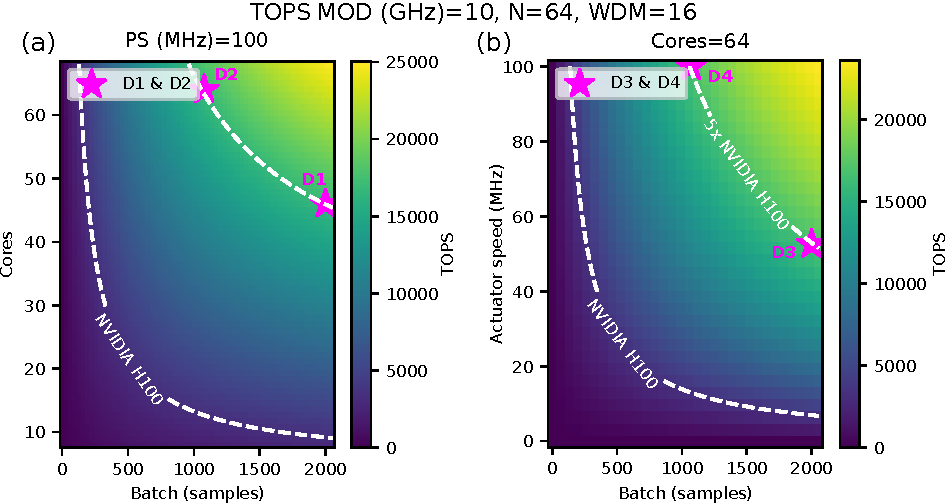
\includegraphics{figures/ch5-compute_tops_batchs.pdf}
	\end{center}
	\caption{TOPS of an optical compute architecture based on MZI meshes and exploiting WDM, multicore and high-speed phase actuators techniques.
		The white contours show the performance for different H100 Nvidia GPUs for reference.
	}\label{fig:ch5-compute_tops}
\end{figure}

The resulting TOPS obtained by sweeping $C$ (\# of cores) with $K$ (batch size) and $f_{PS}$ (phase shifter frequency) with $K$ (batch size) are presented in Figure~\ref{fig:ch5-compute_tops} (a) and (b), respectively.
Note that the white contours also show the TOPS performance of an Nvidia H100 tensor core GPU and a 5x improvement of this metric.
For an optical matrix multiply accelerator to be a viable competitor of conventional electronic GPUs, at low-precision (8 bits) inference workloads, it must at least yield a five-fold improvement with respect to the latter.
Because of this we have chosen four different designs (D) of possible architectures as seen in Table~\ref{tab:ch5-compute_tops}.
To perform this comparison with respect to the H100 system we have chosen a set of fixed ambitious metrics such as a unitary operator of size 64, 16 wavelength carriers \cite{noauthor_cw-wdm_nodate} and a high speed on chip modulator of 10 GHz.
We have chosen 64 as the maximum size of the matrix as our models show that's the maximum size to achieve 8 bit of resolution in an optimized system \cite{ward-foxton_optical_2021}.
This resolution is directly limited by the losses introduced by the chip.

\begin{table}
	\centering
	\caption{Different optical matrix-multiply architectures required to reach 5x performance improvement compared to an Nvidia H100. Both architectures are compared at 8-bit precision performance}\label{tab:ch5-compute_tops}
	\begin{tabular}{|c|c|c|c|c|}
		\hline
		Architecture & \# of Optical Cores & Actuator frequency (MHz) & Bach size & H100 comparison \\
		\hline
		D1           & 46                  & 100                      & 2000      & 5x              \\
		\hline
		D2           & 64                  & 100                      & 1080      & 5x              \\
		\hline
		D3           & 64                  & 52.6                     & 2000      & 5x              \\
		\hline
		D4           & 64                  & 100                      & 1070      & 5x              \\
		\hline
	\end{tabular}
\end{table}

The results show that even for a relatively large batch size (typical values are around 128 due to memory bandwidth limitations \cite{noauthor_llm_2023}) the systems need a very fast phase shifter with a rise time in the sub ns range and a massive multicore approach (> 46) to achieve a performance 5 times the one of a single H100 card \cite{noauthor_nvidia_nodate}.
When we compare this with a multicore GPU systems such as the DGX H100 system that contains 8 H100 cards with a performance of 32 petaOPS (i.e., 9.7x that of an H100 card) the picture becomes grimmer \cite{noauthor_nvidia_nodate-1}.

The pros of the optical solution are the high encoding frequency of optical modulators and low propagation latency given by the propagation of light in silicon.
The cons, however, overshadow the latter because on one hand the losses and bulkiness of silicon photonics limit the maximum operator size which in turn means that large matrices have to be split in numerous tiles to be optically implemented.
On the other hand, the relatively slow phase changing effect (constrained in turn to yield the lowest losses possible) severely limits the refresh speed of weights in the matrix and impacts negatively the system's performance.
Another big problem is the need to move data from the digital domain to the analog and back to the digital \cite{meech_data_2023} which introduces costly conversions and limits the resolution.
These are the reasons we observe the need of a massive multicore, multiwavelength architecture to the performance of a single H100 card.
Of course, these solutions involve non-trivial technical challenges, don't scale well and can't match the metrics of their electronic multicore counterparts such as the DGX H100 or the NVL72.
Perhaps this is the reason several optical compute startups have changed their value propositions and moved to data movement instead.
It's true that current AI boom required faster, cheaper and more energy efficient solutions that can enable the democratization and application build-up of AI technology.
The evidence suggests that the current systems' bottleneck is not on the compute side, but rather on the enormous data flow requirements of AI \cite{cole_optical_2021} and this is where this kind of silicon photonics MZI meshes stand higher chances to find a killer app.
For pure photonic computing to become competitive, researchers must find additional avenues in high-speed (>30GHz) time domain computing capabilities in order to truly leverage on the very high bandwidth capabilities of optics \cite{tsakyridis_photonic_2024}.
We must recall, however, that an all-optical solution is not realistic making an optoelectronic approach the only option left, for which the aforementioned tradeoffs must be considered seriously.
% section Optical computing (end)
\section{Conclusions}\label{sec:conclusions} % (fold)

% - The achievements of this thesis
% - Full tech stack system
% - Summary of applications with refs
This dissertation covers the developments made to design, fabricate and assemble a multipurpose programmable photonics platform powered by a reconfigurable silicon on insulator chip.
The activities carried out during this research touched different points of the technology stack with special emphasis on the layout design of the chip, the control electronics and the software control layer to interact with the silicon core.
As a result of three years of work and a team of enthusiastic hardworking engineers and scientists the iPronics first-generation Smartlight platform was made commercially available in December 2022 and publicly presented at OFC 2023.
The published applications demonstrated on the same commercial platform span several fields: microwave photonics \cite{perez_multipurpose_2017, perez-lopez_general-purpose_2024,catala-lahoz_self-configuring_2023}, topological photonic arrays \cite{on_programmable_2024,hashemi_non-hermitian_2024}, beamforming networks \cite{perez-lopez_programmable_2018}, optical computing architectures \cite{ashtiani_photonic_2023,ashtiani_universal_2024,ashtiani_programmable_2024}, datacom networking \cite{xie_software-defined_2024}, among others.
Some of these demonstrators have been the first of their kind and therefore have been published in world-class journals.
Moreover, several groups of researchers around the globe are currently prototyping and working on new applications using this platform.

% - Emphasis on Software stack and capabilities
% - Synthesis and configuration algorithms
% - Python API
% - Fast API
Although the first months of this thesis focussed on chip layout and design, the big majority of the work carried out was related to the software control layer and demonstration of applications.
As covered in chapter 3, the activities dealt with the creation of several abstraction layers on top of the silicon chip to create a human-readable interface that would allow configuring and synthesizing different applications on the chip.
The software stack encompasses the orchestration of the control and monitoring electronics, a temperature controller (TEC) and other peripherals through a logic unit (LU) that hosts the algorithms and routines to boot and drive the system.
Among the key routines stored here we found the calibration, the manual configuration and automatic configuration algorithms, and hardware maintenance processes.
A special emphasis was made on the manual and automatic configuration where the former relies on automatically retrieved cached calibration information for the different PUCs and the latter implements an additional graph-based abstraction layer to find the optimum circuit for a given high-level request and a figure of merit.
The algorithms are accessible to the user via a Python API which, alongside other auxiliary tools like core, power and spectrum monitors, serves as a powerful yet user-friendly SDK to prototype several applications.
The Python API serves as a way to interact directly with the standalone system much like the Arduino IDE \cite{noauthor_software_nodate} or Vivado Suite \cite{noauthor_amd_nodate} bridge the human with the microcontroller or FPGA, respectively.
If the system is meant to be used in conjunction with other systems and all of them have to be controlled synchronously by an operator (e.g., a lab environment), a FAST-like API \cite{noauthor_fastapi_nodate} is more sustainable for application testing and deployment.

% - Prospects of the field
% - multipurpose for research: Nokia bell labs papers
% - volume consumption requires application specific
% - Potential killer applications volume
Looking forward to the future of this technology platform we foresee that it will continue to be a key enabler of new application prototyping.
While the standard way of prototyping new applications requires the design and fabrication of ASPIC chips, the multipurpose platform documented in this thesis offers a cheaper and faster alternative to do something similar on a configurable chip.
We must recall, however, that the speedup of development cycles comes with the tradeoff of slightly worse specs due to spurious effects in mesh-based systems.
In most cases though, these effects can be counteracted using the built-in software layer and user-defined routines.
In addition, hardware improvements are becoming progressively reachable.
Reducing the insertion loss for wideband operation \times 4 times, while keeping low first-order crosstalk levels, is already attainable with optimized building blocks.
Nevertheless, for these devices to be deployed in volume, an application with a sizeable market needs to be found first through the prototyping and test trials R\&D groups are currently running.
The existence of a potential "killer app" should be determined in the upcoming years.
A couple of good ways to facilitate the quest for new applications might be open sourcing the chip architecture and instruction set as well as defining standards on the API level so that more researchers can contribute and lead to the formation of a community such as the RISC-V project \cite{noauthor_risc-v_nodate}.
In the meantime we forecast that in the short and mid terms most companies will focus on programmable ASPIC solutions for fields like computing \cite{noauthor_akhetonics_nodate}, chip-to-chip interconnects \cite{noauthor_celestial_nodate,noauthor_passage_nodate}, optical circuit switching \cite{noauthor_ipronics_nodate, noauthor_salience_nodate}, LiDAR \cite{noauthor_opa_2021}, among others.
As these solutions become more pervasive, their need for testing and prototyping using multipurpose PICs is expected to grow in the long run either as standalone development systems or IP blocks.

% section Conclusions (end)
\section{Future work}\label{sec:future_work} % (fold) 
\subsection{Photonic hardware defined language}\label{sub:phdl} % (fold)

Hardware Description Languages (HDLs) like Verilog and VHDL are essential for designing and simulating digital circuits, enabling engineers to model complex hardware systems at various abstraction levels.
HDLs provide a platform for describing Register-Transfer Level (RTL) designs, allowing for precise control over data flow, timing, and hardware behavior.
Their use is critical in modern workflows as they offer the ability to simulate and verify designs before physical implementation \cite{katz_contemporary_2005}.
Furthermore, HDLs bridge the gap between high-level design concepts and physical hardware by enabling synthesis into gate-level structures and deployment onto chips or programmable logic devices \cite{pedroni_circuit_2004}.
This capability makes them indispensable for both rapid prototyping and large-scale production.

FPGAs synthesize HDL code by transforming high-level hardware descriptions into configurations for the FPGA's programmable logic.
The process begins with synthesis tools, which compile HDL code into a netlist of logic gates optimized for resources and timing.
This netlist is then mapped to the FPGA's architecture, assigning Look-Up Tables (LUTs), flip-flops, and other primitives.
The place-and-route stage determines the physical arrangement and connections within the FPGA, ensuring signal integrity.
Finally, the design is converted into a bitstream file, which programs the FPGA to implement the specified circuit.
Tools like Xilinx Vivado \cite{noauthor_amd_nodate} and Intel Quartus \cite{noauthor_fpga_nodate} streamline this process, enabling efficient realization of custom hardware designs.

The case for a Photonic Hardware Description Language (PHDL) is very similar to its electronic counterpart.
On one hand, we have a set of primitives (e.g., tunable couplers, modulators, photodetectors, splitters, etc.) that can be connected with each other to create complex circuits.
And on the other hand we have either a multipurpose mesh that can connect all these elements together (in an FPPGA system) or a set of waveguide connectors that help to place and route the optical components (in an ASPIC system).
If such circuits can be described in terms of a netlist such electronic ICs then they could also be described/synthesized using a higher abstraction level, i.e., a PHDL, and interconnected using the same principles \cite{lee_algorithm_1961}.
Such abstraction layer has to consider the non-trivial aspect that photonic ICs are analog instead of digital, which introduces new design constrains.
Of course this also means that a synchronous description of the hardware behavior such as RTL would not be of much use for PHDLs.
As PICs circuits are in many cases based on interferometry and phase control, a PHDL implementation would need to strongly enforce length equalization and path length difference to work appropriately.
The synthesis of PHDL code should also minimize waveguide lengths and crossings as they introduce critical loss/phase and optical crosstalk parasitics, respectively.
Attempts in the electronic field to implement analog HDLs based on modern languages such as Python \cite{fritchman_integrated_2023} should be used as reference.
A first implementation of PHDLs could focus on synthesizing and connecting different primitives in a multipurpose mesh such as the one presented in Chapter~\ref{chap:applications_using_fppgas} where path lengths are discrete by design.
The abstraction could then be upgraded and generalized to the design of complex ASPICs following the principles of \cite{lee_algorithm_1961} and taking into account the constraints of optics.

% subsection Photonic hardware defined language (end)
\subsection{Amplification}\label{sub:amplification} % (fold)

% The problem is losses from silicon
Losses in silicon photonics chips significantly impact performance and efficiency.
These losses arise from factors like waveguide sidewall roughness, mode mismatches and material absorption.
Mitigation strategies include advanced fabrication techniques, optimized waveguide, components and coupler designs.
In spite of this, as PICs become larger the insertion losses build-up up to the point where their use in commercial applications becomes very difficult.
% Some kind of compensation is needed for which SOA are ideal or edwas
For this reason, some kind of compensation is needed to retrieve the signal to functional levels.
The perfect candidates for the compensation are semiconductor optical amplifiers (SOA) as they are mature, can be miniaturized and produced in volume.
Erbium-doped waveguide amplifiers (EDWA) promise to be a good alternative once they reach maturity and volume manufacturing \cite{noauthor_edwatec_nodate,liu_photonic_2022}.
% Active introduces nonidealities
In any case, the introduction of active elements in the system will also bring nonidealities into play.
The effects of the latter have been studied in microwave photonics \cite{sanchez_modeling_2021}, telecom \cite{bonk_soa_2018} and datacom networks \cite{o_duill_estimation_2017, way_technical_2014,maharry_integrated_2023}.
The studies show that it's important to develop techniques to suppress waveform distortion when driving the active elements \cite{masumoto_approach_2022}.
Among the key metrics that will have to be optimized when amplifiers are introduced to compensate chip losses we have: signal-to-noise ratio (SNR), bit-error ratio (BER) and transmitter dispersion eye closure (TDECQ), for PAM4 signals.
Different types of amplifiers will need to be optimized and compared between each other to ensure the highest signal quality \cite{st-arnault_performance_2024} at the system's output.
If the application handles WDM signals then the flatness of the chip's transmission response and the amplifier's spectral mask will need to co-designed and refined ensemble.

% subsection Amplification (end)
\subsection{Circuit aware calibration}\label{sub:circuit_aware_calibration} % (fold)

As covered in Chapter~\ref{chap:universal_unitary_operators}, when synthesizing phase-sensitive circuits in the mesh, the spectral response of the hardware doesn't match with the simulation results \cite{on_programmable_2024,sanchez_gomariz_scalability_2024}.
It was observed that although hardware and simulation match well for circuits depending on coupling factor \( k\) alone (e.g., interconnects, beamsplitters), there are mismatches with circuits that imply interferometry (phase-dependency) such as filters and multiport interferometers \cite{zand_effects_2020}.
This led to the formulation of a new model for the PUC presented in Section~\ref{sub:updated_puc_model} to consider the passive phase introduced by PUC connections.
In Chapter~\ref{chap:universal_unitary_operators}, we covered how these phases could be calibrated for super PUC structures, however other structures such as ring arrays and IIR/FIR filters will still require a calibration routine of their own to work correctly.
This brings two options to the table as follow-up actions: either a calibration routine needs to be run for each phase-sensitive circuit, which encompass a very large subset of structures, or the \(\phi^u_p\) and \(\phi^l_p\) values of each PUC need to be characterized beforehand, so they can be compensated in every circuit.
The first approach is rather straightforward as we only need to make sure that a phase offset is added to individual interferometric structures for them to match their expected response as done in \cite{on_programmable_2024}.
The problem with this approach is that it requires to create a routine for each different circuit as the passive phases involved in each one will be different.
The second approach requires finding enough independent equations (i.e., circuits) so that \(\phi^u_p\) and \(\phi^l_p\) can be determined for the entire mesh solving a linear equations' system.
With this information, any phase-sensitive circuit can be compensated automatically during the synthesis without the need of a per-case calibration.
The issue with this option is that finding enough equations to identify these variables can be a non-trivial task and requires the implementation of a fully automated process that can be used in several circuits to infer phase drifts in terms of different observable variables.
A third, and more complicated approach is to use on-chip photodetectors, so the user can implement self calibration algorithms such as resonance positioning using the inputs from these PDs.
The problem with this approach is that it introduces more losses and significant fabrication complexity.
In most cases, the use of a phase-sweep routine (approach 1) might be enough and faster to implement to start prototyping the application of interest.
Nevertheless, as this kind of recirculating meshes are ported to other platforms \cite{kim_programmable_2023,zhang_compact_2024,zhang_programmable_2025} and the arrays grow larger this issue will have to be addressed.
% subsection Circuit aware calibration (end)

% section Future work (end)
% chapter Discussion and Conclusions (end)

% Author: David Sanchez-Jacome

\chapter*{Author's merits} \label{sec:merits}
\addcontentsline{toc}{chapter}{Author's merits}

% \begin{noindent}
\section*{Journal publications}

\begin{itemize}
  \item M. B. On, F. Ashtiani, \textbf{D. Sanchez-Jacome}, et al., "Programmable integrated photonics for topological Hamiltonians," \textit{Nat. Commun.}, vol. 15, no. 629, 2024. doi: \href{https://doi.org/10.1038/s41467-024-44939-3}{10.1038/s41467-024-44939-3}.
  \item D. Pérez-López, A. Gutierrez, \textbf{D. Sánchez}, et al., "General-purpose programmable photonic processor for advanced radiofrequency applications," \textit{Nat. Commun.}, vol. 15, no. 1563, 2024. doi: \href{https://doi.org/10.1038/s41467-024-45888-7}{10.1038/s41467-024-45888-7}.
  \item Z. Xie, \textbf{D. Sánchez-Jácome}, L. Torrijos-Morán, and D. Pérez-López, "Software-defined optical networking applications enabled by programmable integrated photonics," \textit{J. Opt. Commun. Netw.}, vol. 16, pp. D10-D17, 2024. doi: \href{https://doi.org/10.1364/JOCN.521505}{10.1364/JOCN.521505}.
  \item I. Teofilovic, A. Cem, \textbf{D. Sanchez-Jacome}, D. Pérez-López and F. Da Ros, "Thermal Crosstalk Modelling and Compensation Methods for Programmable Photonic Integrated Circuits," in
    \textit{Journal of Lightwave Technology}, vol. 42, no. 22, pp. 7816-7824, 15 Nov.15, 2024, doi: \href{https://doi.org/10.1109/JLT.2024.3430504}{10.1109/JLT.2024.3430504}.
  \item A. Tsirigotis, A. Sarantoglou, S. Deligiannidis, E. Sánchez, \textbf{D. Sanchez}, et al., "Photonic neuromorphic accelerator for convolutional neural networks based on an integrated
    reconfigurable mesh," \textit{Nat. Commun. Eng.}, vol. 4, no. 80, 2025. \href{https://doi.org/10.1038/s44172-025-00416-3}{10.1038/s44172-025-00416-3}.
\end{itemize}

\section*{Conference contributions}

\begin{itemize}
  \item \textbf{D. Sanchez-Jacome}, M. Rodriguez-Losada, E. Sanchez-Gomaris, and D. Perez-Lopez, “Parametric Unitary Operators Experimentally Demonstrated on a Software-Defined Photonic Integrated Processor,” in \textit{2024 European Conference of Optical Communications (ECOC24)}, 2024.
  \item Z. Xie, \textbf{D. Sanchez-Jacome}, L. Torrijos-Moran, and D. Perez-Lopez, “Reconfigurable on-chip optical circuit switch for software-defined networking applications,” in \textit{2024 European Conference of Optical Communications (ECOC24)}, 2024.
  \item A. Tsirigotis, \textbf{D. Sanchez-Jacome}, et al., “Experimental Investigation of a Neuromorphic Accelerator based on Reconfigurable Photonic Chip for High-Speed Image Processing,” in \textit{2024 European Conference of Optical Communications (ECOC24)}, 2024.
  \item A. Cem, \textbf{D. Sanchez-Jacome}, D. Pérez-López, and F. Da Ros, "Thermal Crosstalk Modeling and Compensation for Programmable Photonic Processors," in \textit{2023 IEEE Photonics Conference (IPC)}, Orlando, FL, USA, 2023, pp. 1-2. doi: \href{https://doi.org/10.1109/IPC57732.2023.10360567}{10.1109/IPC57732.2023.10360567}.
  \item \textbf{D. Sánchez-Jácome}, A. Santome-Valverde, and D. Pérez-López, “Programmable Integrated Photonics Circuits: Applications for 5G, Computing, Data Center, Sensing, and Beyond,” in
    \textit{2022 Epixfab Silicon Photonics Summer School}, 2022. \textbf{Received the best poster award}.
  \item D. Pérez-López, A. López Hernández, M. Gutiérrez, \textbf{D. Sánchez-Jacome}, and E. Sánchez, “Dynamically-reconfigurable Photonic Integrated Circuits and Its Control Algorithms,” in \textit{2023 Conference on Lasers and Electro-Optics (CLEO)}, 2023.
  \item \textbf{D. Sánchez-Jácome}, M. Gutiérrez-Zubillaga, Z. Xie, and D. Pérez-López, “Software-defined Synthesis of Optical Circuits on a Programmable Photonic Platform,” in \textit{2023 IEEE Society for Photonics Summer Topics Meeting Series (SUM)}, 2023.
  \item F. Ashtiani, M. B. On, \textbf{D. Sanchez-Jacome}, D. Perez-Lopez, S. J. Ben Yoo, and A. Blanco-Redondo, “Photonic Max-Pooling for Deep Neural Networks Using a Programmable Photonic Platform,” in \textit{Optical Fiber Communication Conference (OFC) 2023}, 2023, paper M1J.6.
\end{itemize}

\section*{Patents}

\begin{itemize}
  \item L. Torrijos-Morán, D. Pérez-López, T. Hoekstra, \textbf{D. Sánchez-Jácome}, and J. Fernández-Vicente, “Optical Networking Device,” submitted to European Patent Office.
\end{itemize}
% \end{noindent}

% Author: David Sanchez-Jacome

\chapter*{About this manuscript} \label{sec:about}
\addcontentsline{toc}{chapter}{About this manuscript}

% \begin{noindent}
This manuscript was written in \href{https://en.wikipedia.org/wiki/LaTeX}{LaTeX} using \href{https://www.tug.org/texlive/}{TeX Live 2025} packages on a GNU/Linux machine running \href{https://system76.com/pop/download/}{Pop!\_OS 22.04 LTS}.
% \end{noindent}
The LaTeX code was compiled with \href{https://mgeier.github.io/latexmk.html}{latexmk v4.86a} using the \href{https://www.luatex.org/}{luaTEX} engine.
The text editor I have used is \href{https://neovim.io/}{Neovim v1.11.1} in which the \href{https://github.com/lervag/vimtex}{VimTeX} plugin has been instrumental providing linting, syntax checking, templates and useful snippets to navigate a LaTeX codebase project.
Writing LaTeX using Neovim was inspired and heavily influenced by \href{https://ejmastnak.com/tutorials/vim-latex/intro/}{this great seven-series guide} as a way to achieve fast and powerful mathematical typesetting.
For \href{https://microsoft.github.io/language-server-protocol/}{language server protocol (LSP)} tooling \href{https://github.com/latex-lsp/texlab}{texlab v.5.22.1} and \href{https://github.com/ltex-plus/ltex-ls-plus}{LTeX+} have served as great complements for VimTeX.
The latter has turned out to be a great tool for enhancing the limited native spelling features of Neovim.
Automatic formatting has been performed by \href{https://github.com/FlamingTempura/bibtex-tidy}{bibytex-tidy v1.14.0} and the great \href{https://github.com/cmhughes/latexindent.pl}{latexindent.pl v3.24.5} Perl script.
The latter has provided me with the very useful feature of one-line-per-sentence wrapping which has not only made my LaTeX code/text more readable but also has helped me to organize and synthesize my ideas when writing them down.
The formatting rules can be found in the `format-latex.yml` file located in the `.github/` directory.
For continuous integration (CI), GitHub actions checking the formatting rules in `format-latex.yml` have been employed on each pull request and push.
The figures in this manuscript have mostly been created/edited using \href{https://inkscape.org/}{Inkscape v1.1} and \href{https://workspace.google.com/products/slides/}{Google Slides}.
The template used for this manuscript was the \href{https://web.mit.edu/thesis/tex/}{MIT thesis template in LaTeX} which provided most of the classes, packages, fonts and file structure needed during the writing process.

Since I have been actively working in collaborative software development for the last 4 years I decided to host this project on a \href{https://github.com/ricarvid1/dsj-thesis}{Github repo} instead of Overleaf.
In my humble opinion, and based on this experience, if a text editor/\href{https://medium.com/@rcpassos/writing-latex-documents-in-visual-studio-code-with-latex-workshop-d9af6a6b2815}{IDE} is provisioned with the right plugins for LaTeX editing, the collaborative features of GitHub far outpace the ones offered by Overleaf.
This \href{https://github.com/ricarvid1/dsj-thesis}{thesis GitHub repo} will be open-sourced after it has been accepted by the UPV library.
For questions and content discussion please raise an issue in this repo.


%%% Appendicies of thesis  %%%%%%%%%%%%%%%%%%%%%%%%%%%%%%%%%%%%%%%%%%%%%%%%%%%%%%%%%%%%%%%%%%%%%%%%

\appendix
% \include{app1-thermal}
% \include{app2-onn}

%%% Bibliography (biblatex)  %%%%%%%%%%%%%%%%%%%%%%%%%%%%%%%%%%%%%%%%%%%%%%%%%%%%%%%%%%%%%%%%%%%%%%

\defbibheading{bibintoc}{\chapter*{#1}\addcontentsline{toc}{backmatter}{\refname}}
% this sets the title of contents name for bibliography to \refname (= References)
% change "backmatter" to "chapter" if you prefer a bold face entry in the table of contents

\printbibliography[title={\refname},heading=bibintoc]

% biblatex also supports chapter-by-chapter bibliography, https://tex.stackexchange.com/a/296502/119566
% see the biblatex manual, section 3.14.3

%%%% Option for natbib %%%%%%%%%%%%%

%%   use an appropriate style (.bst) and your own .bib file[s]

%\bibliographystyle{plainnat}
%\bibliography{mitthesis-sample.bib}

\end{document}

